\chapter{Measurement of Hadronic Production and $\Gamma(\psipptononDD)$}
\label{ch:non_DDbar}

The second half of this analysis concerns the measurement of hadronic production.
Namely, we are examining hadronic events in the regions above the $\DDbar$ threshold (scan data) and below the $\psip$ peak (continuum data).
After identifying the total number of hadronic events in data, we can determine $\xsecpsipptononDDbar$ in the scan region by subtracting off all other known decay processes.
Using this, along with the previous values of $\xsecpsipptoDDbar$, we can measure the $\nonDDbar$ branching fraction:
\beq
\label{eq:nonDDbar_bf}
\Gamma(\psipptononDD) = \frac{ \xsecpsipptononDDbar }{ \xsecpsipptoDDbar + \xsecpsipptononDDbar }.
\eeq

\section{Data and Monte Carlo Samples}
\label{sec:non_DDbar_data_samples}

\subsection{Data Samples}
\label{ssec:data_samples_non_DDbar}

The data used for this analysis was also produced by BEPCII and collected by BESIII.
The samples used include continuum data taken at \SI{3.650}{\GeV} in 2009 (old continuum), as well as multiple other continuum points taken around this energy in 2013 (new continuum).
We also use Round 1 (R1) and Round 2 (R2) of the high-statistics $\psipp$ data taken in 2010 and 2011, respectively.
Each of these samples, and their measured luminosities, can be seen in \Cref{tab:data_samples_non_DDbar}.
The values of luminosity were measured during a previous version of this analysis using the procedure described in \Cref{ssec:luminosity_measurement}.
The labels given to each continuum point are the intended energy targets, but generally differ from their true values.
In addition to these datasets, the scan data described previously (\Cref{ssec:data_samples}) is also used.


\subsection{Center-of-Mass Energy Measurement}
\label{ssec:energy_measurement_non_DDbar}

As before, a precise measurement of each energy point is vital to the accuracy of the final results.
Most notably, due to the rapidly increasing shape of the $\psip$ cross section near the high end of the continuum points, the value of the 3671 (New) point is highly susceptible to the assumed cross section of the $\psip$.
Following the procedure of \Cref{ssec:energy_measurement}, we measured the $\Ecm$ value of each continuum point.
This resulted in a \SIrange{4}{6}{\MeV} shift downwards for each of the new continuum points, but virtually no shift for the old continuum point.
The measured energies and luminosities of each sample are shown in \Cref{tab:data_samples_non_DDbar}.


\begin{table}[H]
\centering
\renewcommand\arraystretch{1.0}
\begin{tabular}{l|c r}
\hline
Sample Name & $\Ecm$ [\si{\GeV}] & Luminosity \si{\invpb} \\
\hline
3500 (New)    & 3.496 & \num{  3.680 \pm 0.009} \\
3542 (New)    & 3.538 & \num{  3.481 \pm 0.009} \\
3600 (New)    & 3.596 & \num{  0.395 \pm 0.019} \\
3650 (New)    & 3.644 & \num{  5.420 \pm 0.009} \\
3671 (New)    & 3.665 & \num{  4.669 \pm 0.009} \\
3650 (Old)    & 3.650 & \num{ 44.334 \pm 0.009} \\
$\psipp$ (R1) & 3.773 & \num{926.922 \pm 0.092} \\
$\psipp$ (R2) & 3.773 & \num{1978.92 \pm 0.091} \\
\hline
\end{tabular}
\caption{Data samples used for the inclusive measurement.}
{While the 3600 (New) sample was intended to be similar in luminosity to the other continuum points, accelerator issues inhibited the data collection procedure. 
The new continuum points also have a much smaller luminosity compared to the other datasets used in this analysis.}
\label{tab:data_samples_non_DDbar}
\end{table}


\section{Event Selection}
\label{sec:non_DDbar_event_selection}

In order to select the number of hadronic events in each sample, we apply a variety of cuts.
For charged tracks in the MDC, these include the cuts shown in \Cref{tab:charged_cuts_non_DDbar}.

\begin{table}[H]
\centering
\renewcommand\arraystretch{1.0}
\begin{tabular}{c| r@{$\; < \;$}l}
\hline
Vertex ($xy$) & $V_{xy}$ & \pp \SI{1}{\cm} \\
Vertex ($z$)  & $|Vz|$   & \SI{10}{\cm} \\
MDC Angle & $|\cos\theta|$ & 0.93 \\
\hline
\end{tabular}
\caption{Selection cuts on charged tracks used to count hadronic events.}
\label{tab:charged_cuts_non_DDbar}
\end{table}

For neutral tracks in the EMC, these include the cuts shown in \Cref{tab:neutral_cuts_non_DDbar}.

\begin{table}[H]
\centering
\renewcommand\arraystretch{1.0}
\begin{tabular}{c|l r}
\hline
Minimum Energy (Barrel) & $E_{\text{EMC}} > \SI{25}{\MeV}$ & $(|\cos\theta| < 0.80)$ \\
Minimum Energy (Endcap) & $E_{\text{EMC}} > \SI{50}{\MeV}$ & $(0.86 < |\cos\theta| < 0.92)$ \\
TDC Timing & $(0 \leq t \leq 14) \times \SI{50}{\ns}$ & \\
\hline
\end{tabular}
\caption{Selection cuts on neutral tracks used to count hadronic events.}
\label{tab:neutral_cuts_non_DDbar}
\end{table}


To reject background events of $\bhabha$ or $\ee \rightarrow \gamma\gamma$, we also employ cuts related to the highest energy and highest momentum tracks in the event.
These are listed in \Cref{tab:bhabha_cuts_non_DDbar}.

\begin{table}[H]
\centering
\renewcommand\arraystretch{1.0}
\begin{tabular}{l|l@{}l l@{}l}
\hline
\multirow{4}{*}{Highest Energy}   & $\cosmax_+ <  $ & 0.8                            & \multirow{2}{*}{($\Ntrk$} & \multirow{2}{*}{ = 2)} \\
                                  & $\cosmax_- > -$ & 0.8                            & & \\
\cline{2-5}
                                  & $\cosmax_+ <  $ & 0.8 or $\pEmax_+ \leq 0.3$     & \multirow{2}{*}{($\Ntrk$} & \multirow{2}{*}{ = 3, 4)} \\
                                  & $\cosmax_- > -$ & 0.8 or $\pEmax_- \leq 0.3$     & & \\
\hline
\multirow{2}{*}{Highest Momentum} & \multicolumn{2}{l}{$0.8 \leq \Epmax_+ \leq 1.1$} & & \\
                                  & \multicolumn{2}{l}{$0.8 \leq \Epmax_- \leq 1.1$} & & \\
\hline
\end{tabular}
\caption{Selection cuts to remove Bhabha and two-photon backgrounds.}
{The $_+$ and $_-$ denote positively and negatively charged tracks, respectively.  The $^{\text{max}}$ notation indicates the highest energy or momenta track for the corresponding charge.  The energy cuts depend on the total number of charged tracks in the event, $\Ntrk$.}
\label{tab:bhabha_cuts_non_DDbar}
\end{table}

After applying these sets of cuts, there are three groups of cuts which are considered: Standard (SHAD), Loose (LHAD), and Tight (THAD).
For the nominal procedure, SHAD is used, while LHAD and THAD are for future systematic considerations.
The cuts included in each of these sets are shown in \Cref{tab:shad_cuts_non_DDbar,tab:lhad_cuts_non_DDbar,tab:thad_cuts_non_DDbar}.
These apply to the number of charged tracks ($\Ntrk$), the visible energy ($\Evis$), the total visible momentum in the $z$-direction ($\pzvistot$), the maximum shower energy ($\Eemcmax$), and the total shower energy ($\Eemctot$).
Here, `visible' refers to the sum over charged and neutral tracks.

\begin{table}[H]
\centering
\renewcommand\arraystretch{1.0}
\begin{tabular}{l|r@{ }l l}
\hline
Number of Tracks                     & $\Ntrk$ & $ > 2$               &                  \\
\hline
Visible Energy                       & $\EvisE$ & $ > 0.3$            &                  \\
\hline
Visible Momentum                     & $\pzEvis$ & $ < 0.6$           & $(\Ntrk = 3, 4)$ \\
\hline
Maximum Shower Energy                & $\EemcEmax$ & $ < 0.75$           & $(\Ntrk = 3, 4)$ \\
\hline
\multirow{2}{*}{Total Shower Energy} & \multicolumn{2}{c}{$0.25 < \EemcEtot < 0.75$} & $(\Ntrk = 3)$ \\
                                     & \multicolumn{2}{c}{$0.15 < \EemcEtot < 0.75$} & $(\Ntrk = 4)$ \\
\hline
\end{tabular}
\caption{Standard selection cuts (SHAD) for counting hadronic events.}
\label{tab:shad_cuts_non_DDbar}
\end{table}

\begin{table}[H]
\centering
\renewcommand\arraystretch{1.0}
\begin{tabular}{l|r@{ }l l}
\hline
Number of Tracks                       & $\Ntrk$ & $ > 1$               &                  \\
\hline
\multirow{2}{*}{Visible Energy}        & $\EvisE$ & $ > 0.4$            & $(\Ntrk = 2)$    \\
                                       & $\EvisE$ & $ > 0.3$            & $(\Ntrk \geq 3)$ \\
\hline                                 
\multirow{2}{*}{Visible Momentum}      & $\pzEvis$ & $ < 0.3$           & $(\Ntrk = 2)$    \\
                                       & $\pzEvis$ & $ < 0.6$           & $(\Ntrk = 3, 4)$ \\
\hline
\multirow{2}{*}{Maximum Shower Energy} & $\EemcEmax$ & $ < 0.50$           & $(\Ntrk = 2)$    \\
                                       & $\EemcEmax$ & $ < 0.75$           & $(\Ntrk = 3, 4)$ \\
\hline                                 
\multirow{2}{*}{Total Shower Energy}   & \multicolumn{2}{c}{$0.25 < \EemcEtot < 0.75$} & $(\Ntrk = 2, 3)$ \\
                                       & \multicolumn{2}{c}{$0.15 < \EemcEtot < 0.75$} & $(\Ntrk = 4)$    \\
\hline
\end{tabular}
\caption{Loose selection cuts (LHAD) for counting hadronic events.}
\label{tab:lhad_cuts_non_DDbar}
\end{table}

\begin{table}[H]
\centering
\renewcommand\arraystretch{1.0}
\begin{tabular}{l|r@{ }l l}
\hline
Number of Tracks                     & $\Ntrk$ & $ > 3$               &                  \\
\hline
Visible Energy                       & $\EvisE$ & $ > 0.4$            &                  \\
\hline
Visible Momentum                     & $\pzEvis$ & $ < 0.6$           & $(\Ntrk = 4)$ \\
\hline
Maximum Shower Energy                & $\EemcEmax$ & $ < 0.75$           & $(\Ntrk = 4, 5)$ \\
\hline
\multirow{2}{*}{Total Shower Energy} & \multicolumn{2}{c}{$0.15 < \EemcEtot < 0.75$} & $(\Ntrk = 4)$ \\
                                     & \multicolumn{2}{c}{$0.00 < \EemcEtot < 0.75$} & $(\Ntrk = 5)$ \\
\hline
\end{tabular}
\caption{Tight selection cuts (THAD) for counting hadronic events.}
\label{tab:thad_cuts_non_DDbar}
\end{table}

\section{Hadron Counting}
\label{sec:hadron_counting}

In order to determine the total number of hadronic events in each data sample, we use the average velocity in the $z$-direction.
Signal events should have tracks which average to zero around the collision point, while background events will have randomly oriented momenta.
The fits are done using a double Gaussian shape for the signal and a $2^{\text{nd}}$ order polynomial for the background.

\begin{figure}[H]
\centering
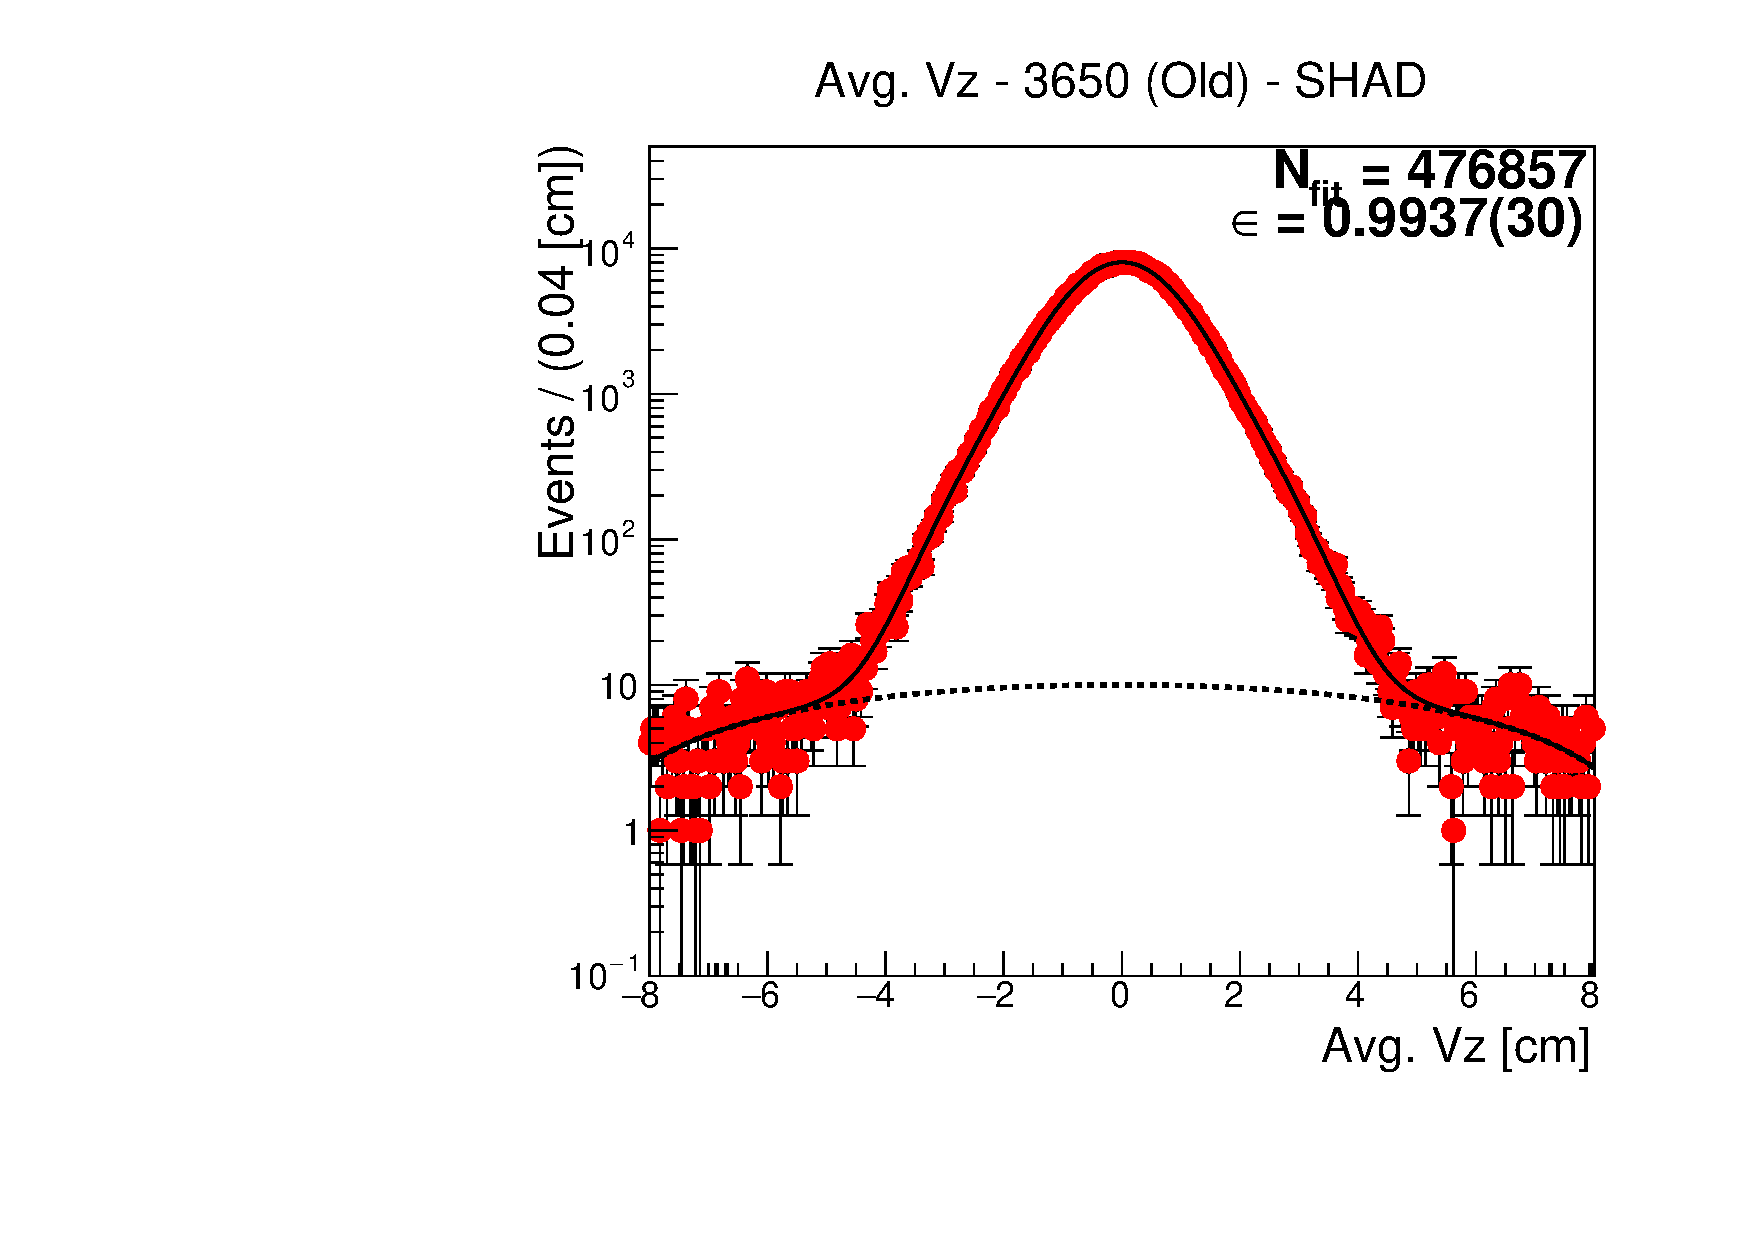
\includegraphics[scale=0.25]{figures/plots/nonDDbar_fit_results/3650_old/fit_old_3650_data_SHAD.pdf}
\hspace{-0.5cm}
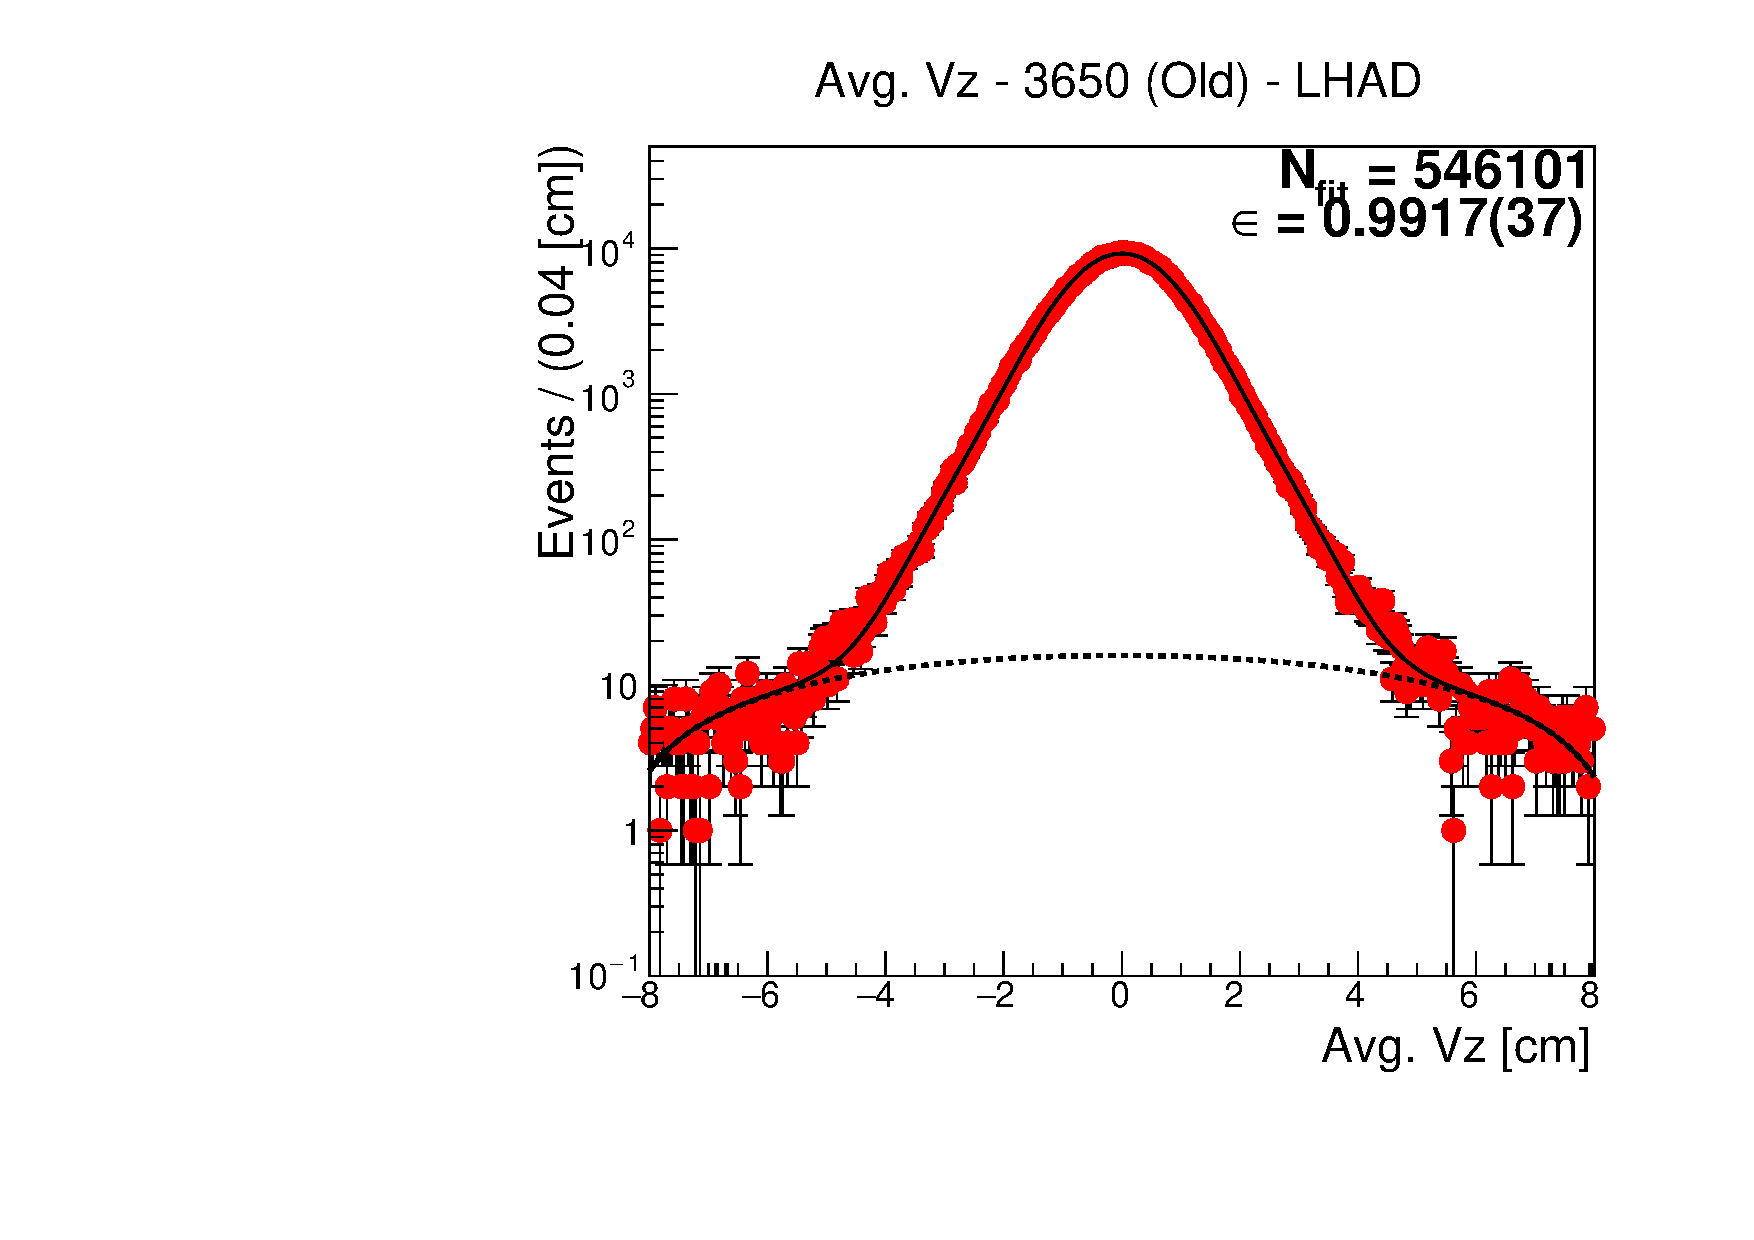
\includegraphics[scale=0.25]{figures/plots/nonDDbar_fit_results/3650_old/fit_old_3650_data_LHAD.pdf}
\hspace{-0.5cm}
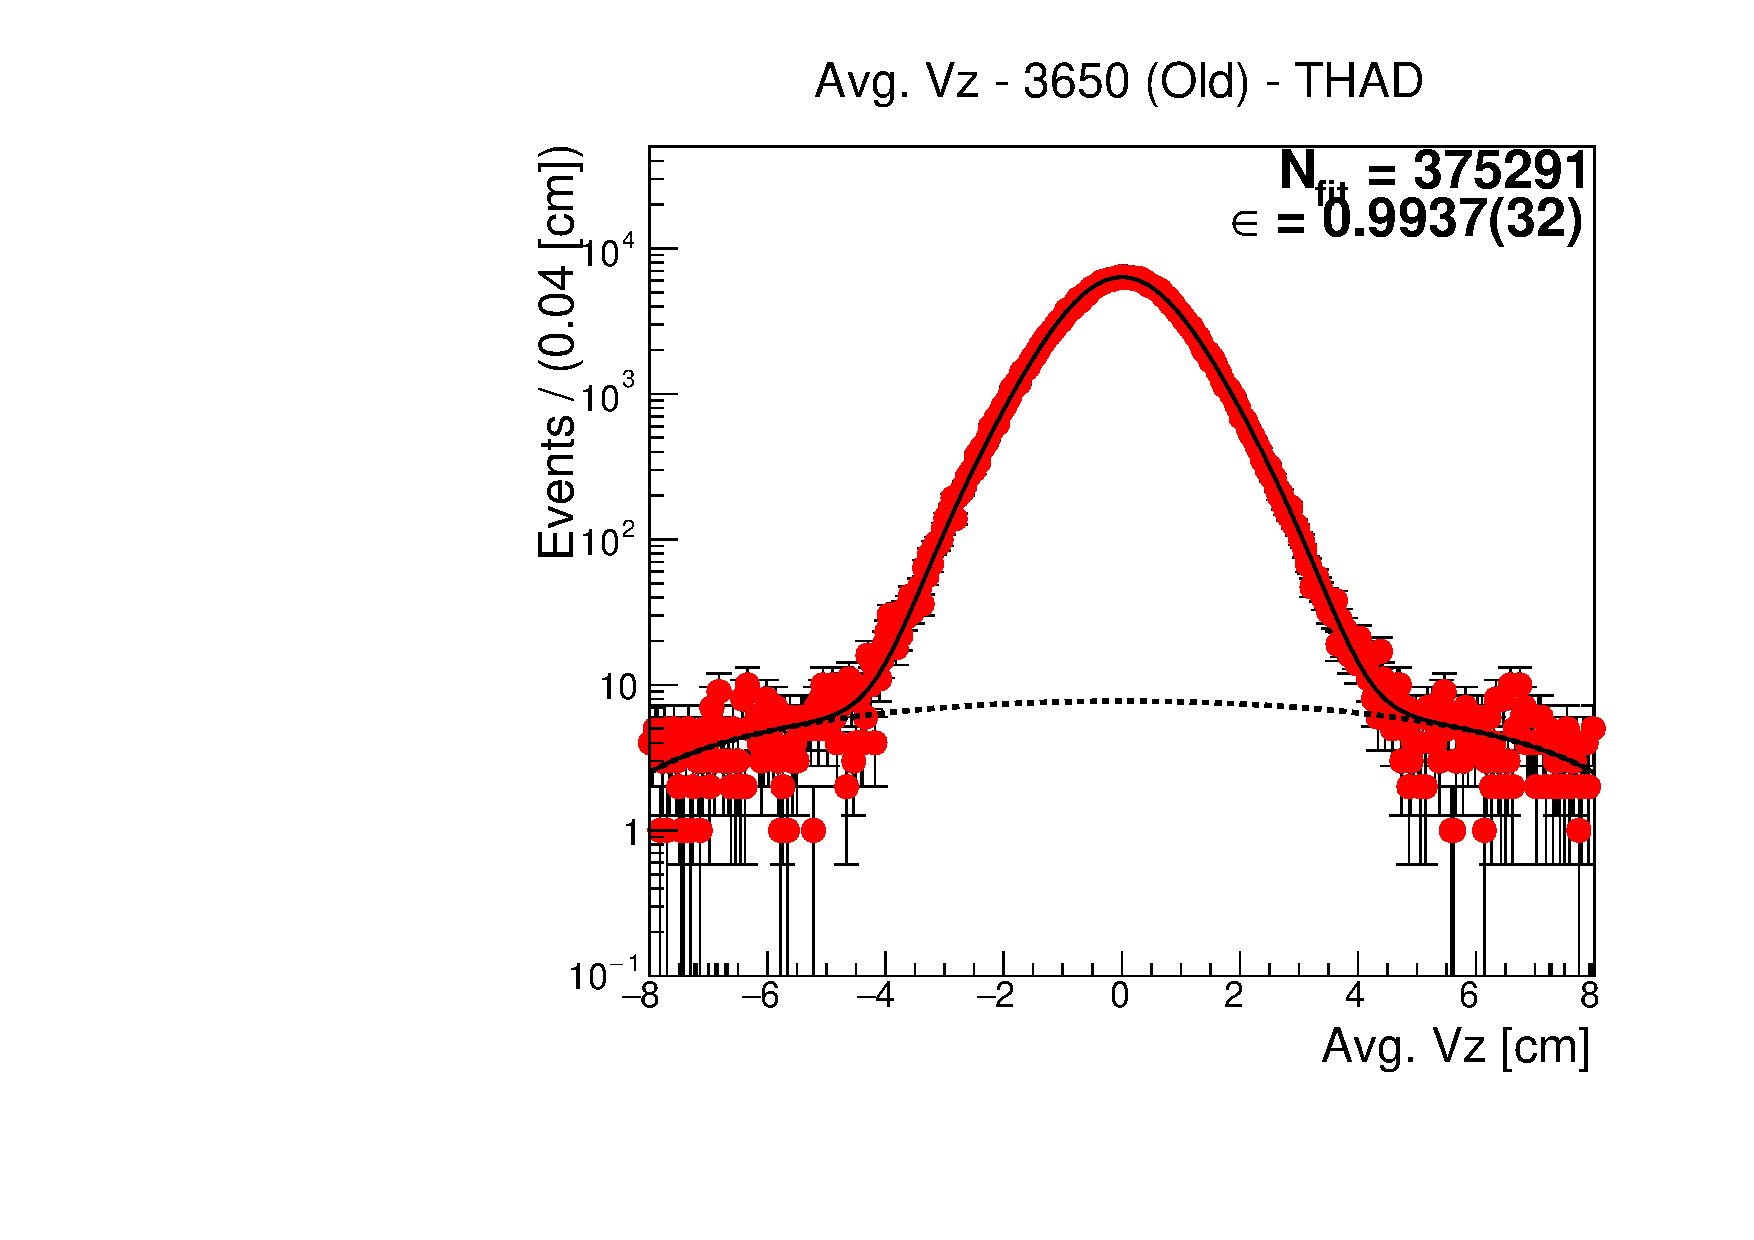
\includegraphics[scale=0.25]{figures/plots/nonDDbar_fit_results/3650_old/fit_old_3650_data_THAD.pdf}
\caption{The number of hadrons found in the 3650 (Old) data sample.}
{This includes results for SHAD (left), LHAD (middle), and THAD (right).}
\label{fig:hadron_fits_3650_old}
\end{figure}


\section{Background Subtraction}
\label{sec:background_subtraction}

To precisely determine the number of hadronic events in the old continuum sample, we must subtract off a variety of backgrounds.
The samples considered for this measurement include two-track QED processes ($\ee$, $\mumu$, $\tautau$, $\yy$), radiative $\jpsi$ ($\yjpsi$), two photon fusion ($\twophoton$), and events coming from $\psip$.
Initially, we assume the $\psip$ has a standard Breit-Wigner shape.

Each background contributes to the total number of reconstructed events based on their cross section ($\sigma$) and reconstruction efficiency ($\effmc$):
\beq
\Nhad = \lum \times \sigma \times \effmc.
\eeq
The efficiency is simply the fraction of reconstructed tracks compared to the total generated in a given MC sample:
\beq
\effmc = \left( \frac{ N_{\text{rec}} }{ N_{\text{gen}} } \right)
\eeq
The MC samples were generated with \num{2.5e3} events for each of the 79 runs in the old continuum data for each of the included backgrounds.
Each sample was analyzed with all three cut selection groups (see \Cref{sec:non_DDbar_event_selection}).
The reconstruction efficiencies for each, along with their cross sections at \SI{3.650}{\GeV} are shown in \Cref{tab:3650_old_reconstruction}.

\begin{table}[H]
\centering
\renewcommand\arraystretch{1.0}
\begin{tabular}{c|r|cr@{$\; \pm \;$}rc cr@{$\; \pm \;$}rc cr@{$\; \pm \;$}rc}
\hline
\multicolumn{14}{c}{3650 (Old) Reconstruction} \\
\hline
Sample & $\sigma$ [\si{\nb}] & \multicolumn{4}{c}{$\effmc$ (SHAD) [\%]} & \multicolumn{4}{c}{$\effmc$ (LHAD) [\%]} & \multicolumn{4}{c}{$\effmc$ (THAD) [\%]} \\
\hline
$\ee$           & 554.562 &&  0.0006 & 0.0002 &&&  0.0008 & 0.0002 &&&  0.0001 & 0.0001 & \\
$\mumu$         &   5.560 &&  0.0033 & 0.0004 &&&  0.0044 & 0.0005 &&&  0.0029 & 0.0004 & \\
$\tautau$       &   1.844 && 12.8351 & 0.0255 &&& 28.7692 & 0.0382 &&&  9.9371 & 0.0224 & \\
$\yjpsi$        &   1.260 && 45.9222 & 0.0482 &&& 55.1722 & 0.0529 &&& 34.1250 & 0.0416 & \\
$\yy$           &  21.530 &&  0.0009 & 0.0002 &&&  0.0010 & 0.0002 &&&  0.0005 & 0.0002 & \\
$\twophoton$    &   1.257 &&  2.4109 & 0.0110 &&&  4.6297 & 0.0153 &&&  1.6468 & 0.0091 & \\
$\psip^\dagger$ &   0.150 && 62.9891 & 0.0078 &&& 69.2882 & 0.0082 &&& 51.6942 & 0.0071 & \\
\hline
\end{tabular}
\caption{Reconstruction of background samples for the old continuum data.}
{These include standard QED two-track processes ($\ee$, $\mumu$, $\tautau$, $\gamma\gamma$), radiative $\jpsi$ ($\gamma\jpsi$) and two photon fusion ($2\gamma$) events, and a contribution coming from $\psip$. \\
$^\dagger$ The $\psip$ is assumed to have a standard Breit-Wigner shape.}
\label{tab:3650_old_reconstruction}
\end{table}

Using each of these values, we can determine the total number of hadronic events in the data.
This is done by subtracting the expected amount of background from the measured number of events passing each selection method in data.
The results for the old continuum data are shown in \Cref{tab:3650_old_results}.
Given that the $\ee$, $\mumu$, and $\yy$ samples have contributions which are much smaller than the uncertainty on the total result, we exclude these from the final calculation.

\begin{table}[H]
\centering
\renewcommand\arraystretch{1.0}
\begin{tabular}{c|cr@{$\; \pm \;$}rc cr@{$\; \pm \;$}rc cr@{$\; \pm \;$}rc}
\hline
\multicolumn{13}{c}{3650 (Old) Results} \\
\hline
Sample         & \multicolumn{4}{c}{$\Nhad$ (SHAD)} & \multicolumn{4}{c}{$\Nhad$ (LHAD)} & \multicolumn{4}{c}{$\Nhad$ (THAD)} \\
\hline
Data            && 477001 & 691 &&& 546546 & 739 &&& 375380 & 613 & \\
$\ee{^*}$       &&    149 &  43 &&&    187 &  48 &&&     12 &  12 & \\
$\mumu{^*}$     &&      8 &   1 &&&     11 &   1 &&&      7 &   1 & \\
$\tautau$       &&  10490 &  30 &&&  23514 &  59 &&&   8122 &  25 & \\
$\yjpsi$        &&  25658 &  60 &&&  30826 &  71 &&&  19067 &  46 & \\
$\yy{^*}$       &&      9 &   2 &&&     10 &   2 &&&      4 &   1 & \\
$\twophoton$    &&   1443 &   7 &&&   2771 &  11 &&&    986 &   6 & \\
$\psip^\dagger$ &&   4175 &   9 &&&   4593 &  10 &&&   3427 &   7 & \\
\hline                                                              
Hadrons         && 435234 & 694 &&& 484842 & 745 &&& 343779 & 615 & \\
\hline
\end{tabular}
\caption{Hadronic events selected in the old continuum data.}
{As expected, SHAD finds less events than LHAD and more than THAD. \\
$^*$ The contribution is neglected for the total results. \\
$^\dagger$ The $\psip$ is assumed to have a standard Breit-Wigner shape.}
\label{tab:3650_old_results}
\end{table}


\section{Efficiency Extrapolation}
\label{sec:efficiency_extrapolation}

Due to complicated interactions above the $\DDbar$ threshold, $\qqbar$ events not coming from $\psipp$ are currently not well modeled by our MC generators.
In order to accurately count these events, we utilize the continuum data, as below the $\psip$ the process is more reliable.
Assuming the production of these events remains consistent over energy, we can use the measurements at lower energies to extrapolate to higher energies:

Measuring the hadronic events for the new continuum data follows exactly as for the old continuum data, but with the negligible backgrounds excluded.
The number of hadrons found in each data sample can be seen in \Cref{fig:hadron_fits_3500_new,fig:hadron_fits_3542_new,fig:hadron_fits_3600_new,fig:hadron_fits_3650_new,fig:hadron_fits_3671_new}.
Reconstruction efficiencies are shown in \Cref{tab:3650_new_reconstruction} with the total results shown in \Cref{tab:3650_new_results}.

\begin{figure}[H]
\centering
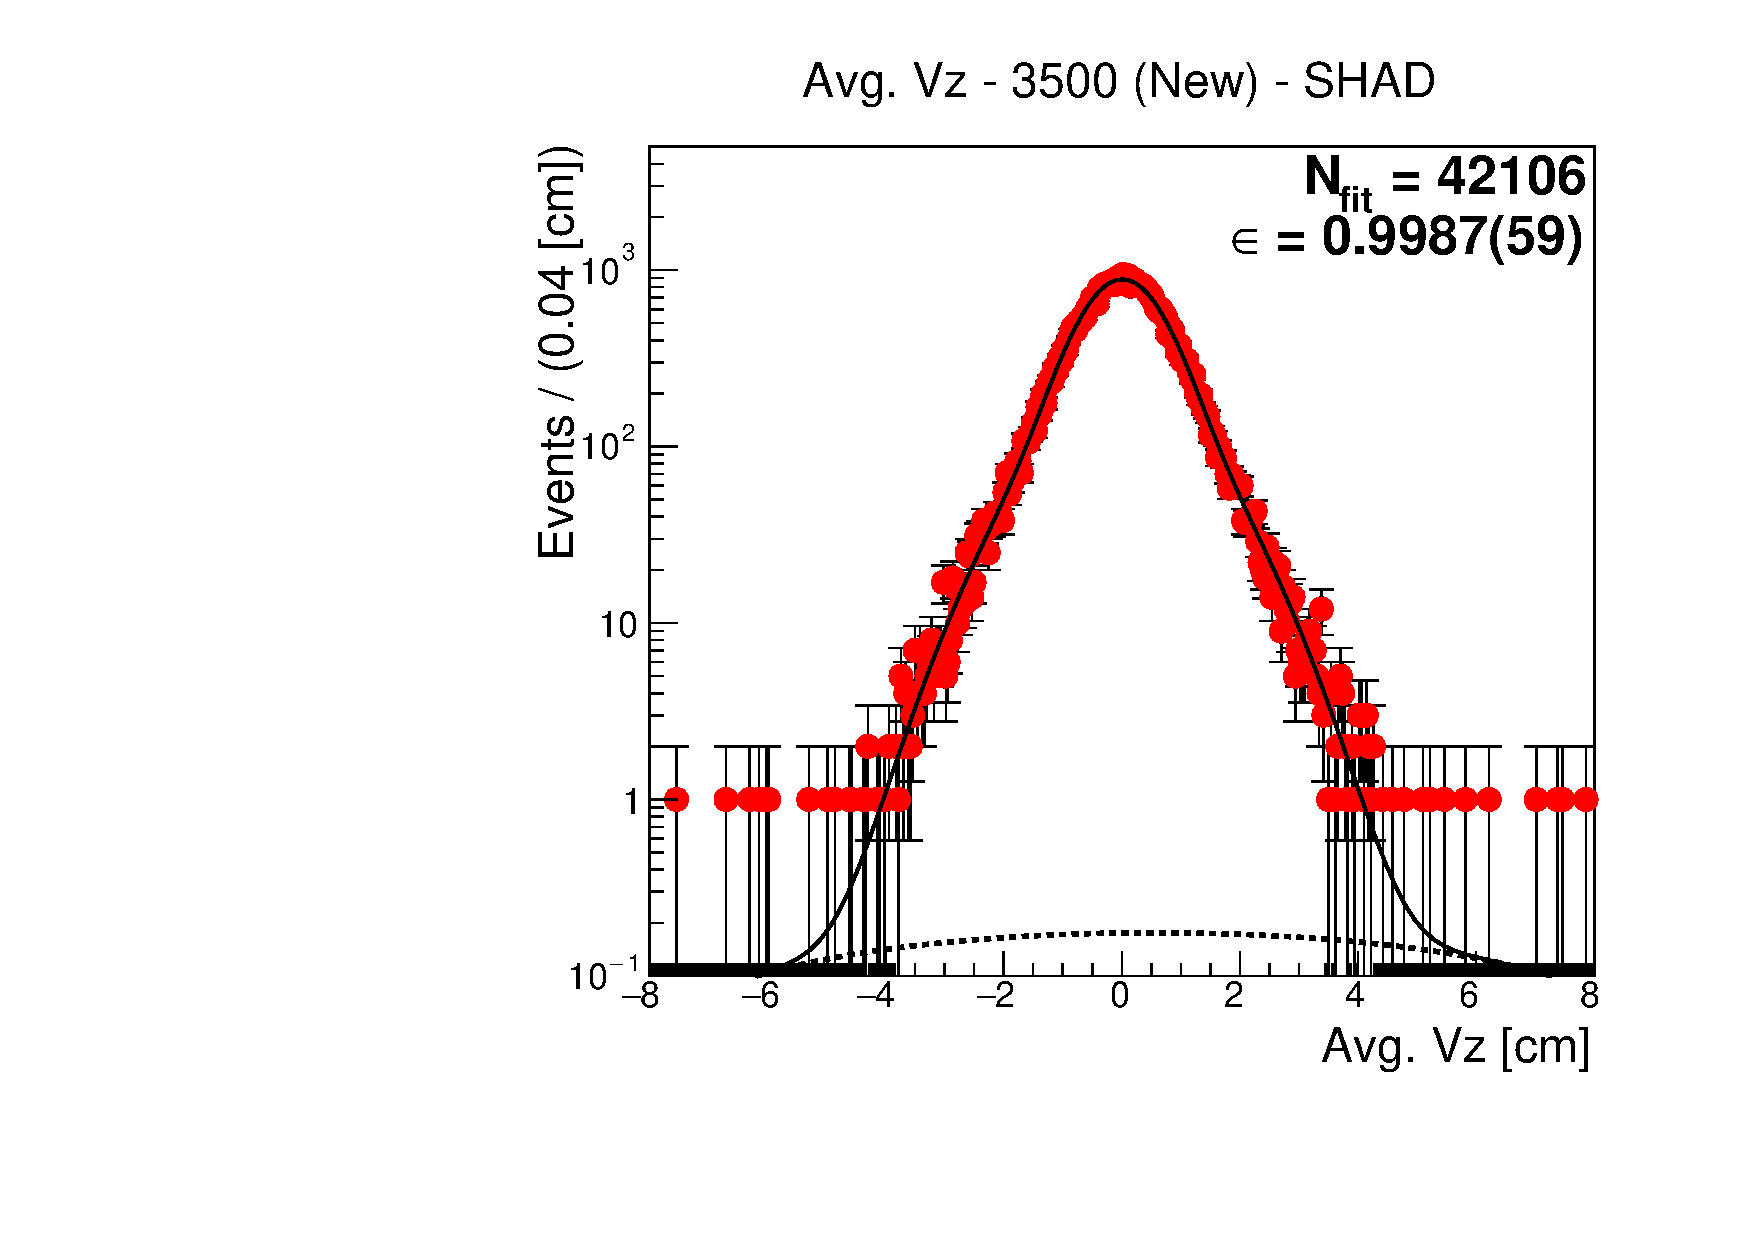
\includegraphics[scale=0.25]{figures/plots/nonDDbar_fit_results/3650_new/fit_new_3500_data_SHAD.pdf}
\hspace{-0.5cm}
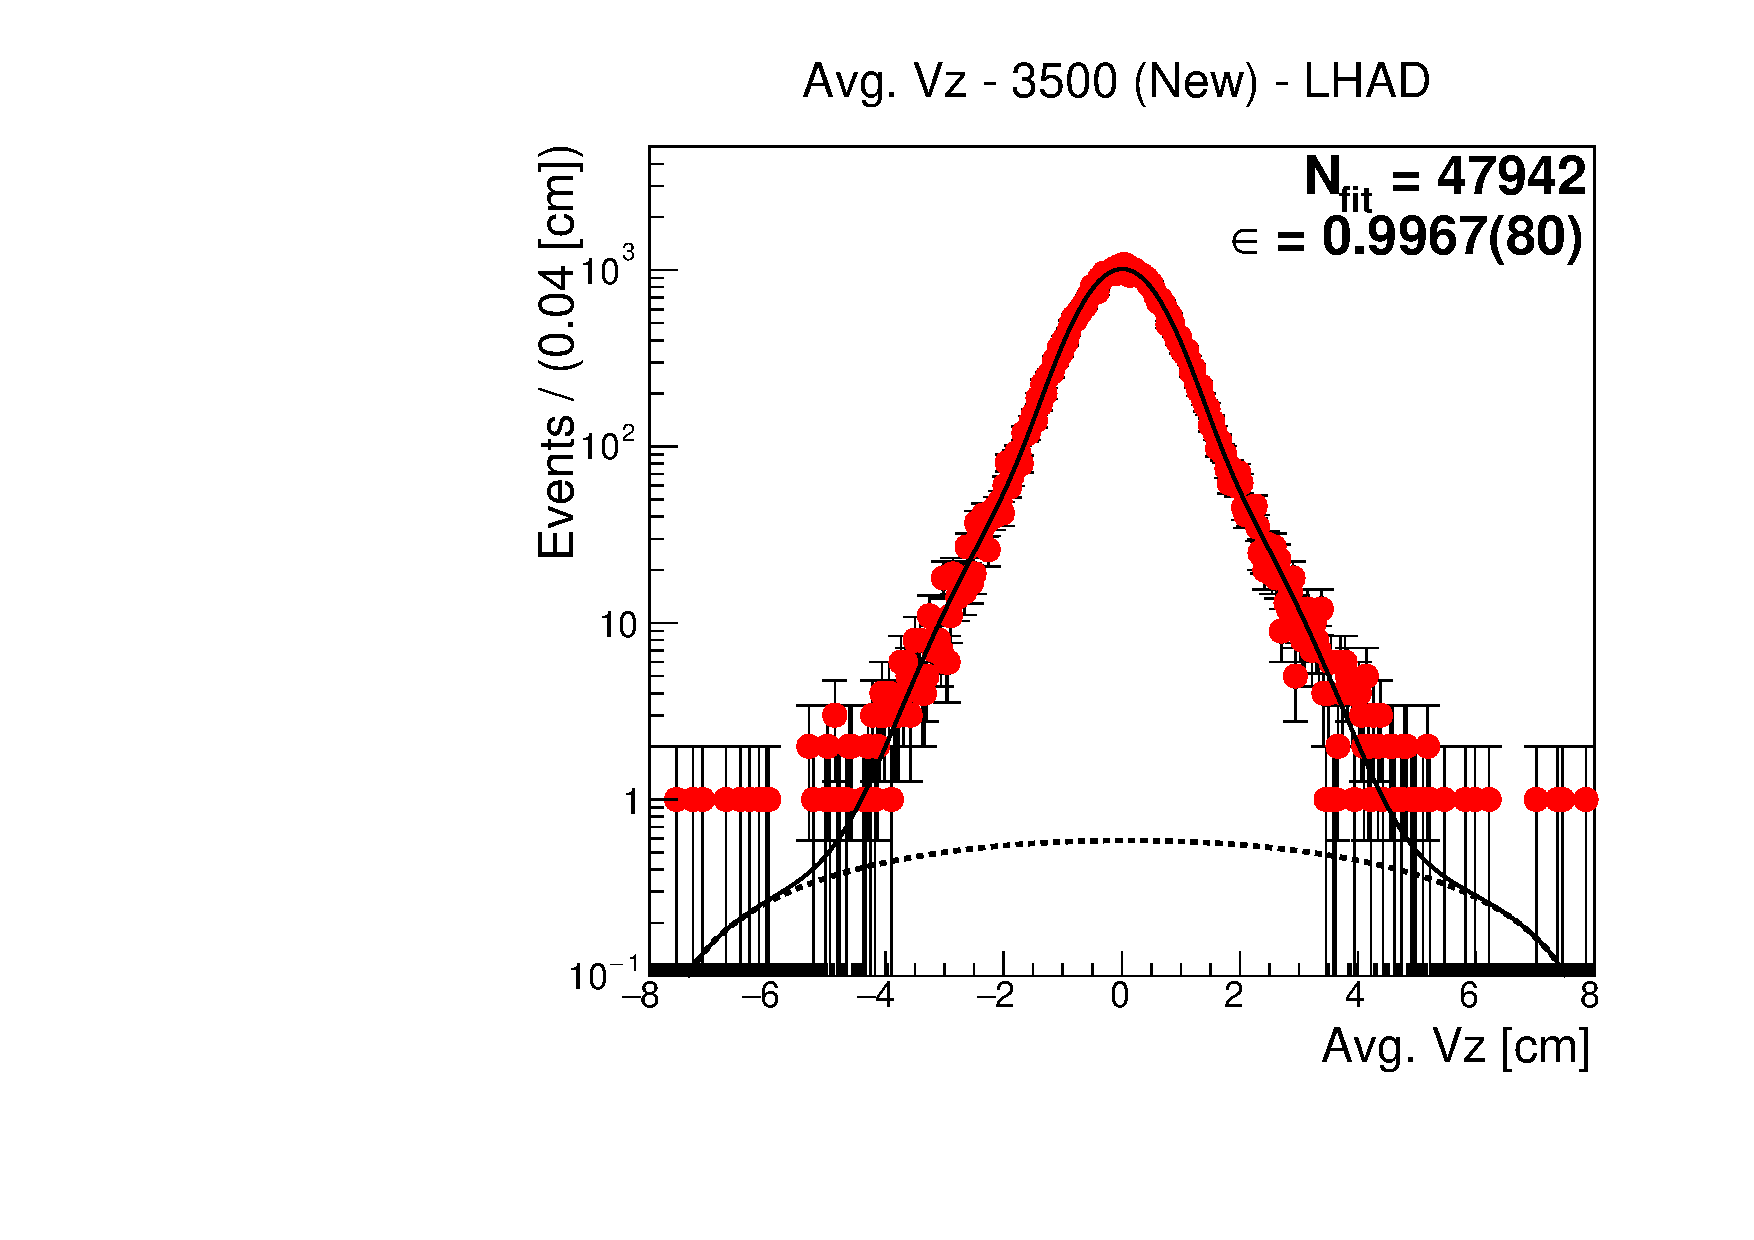
\includegraphics[scale=0.25]{figures/plots/nonDDbar_fit_results/3650_new/fit_new_3500_data_LHAD.pdf}
\hspace{-0.5cm}
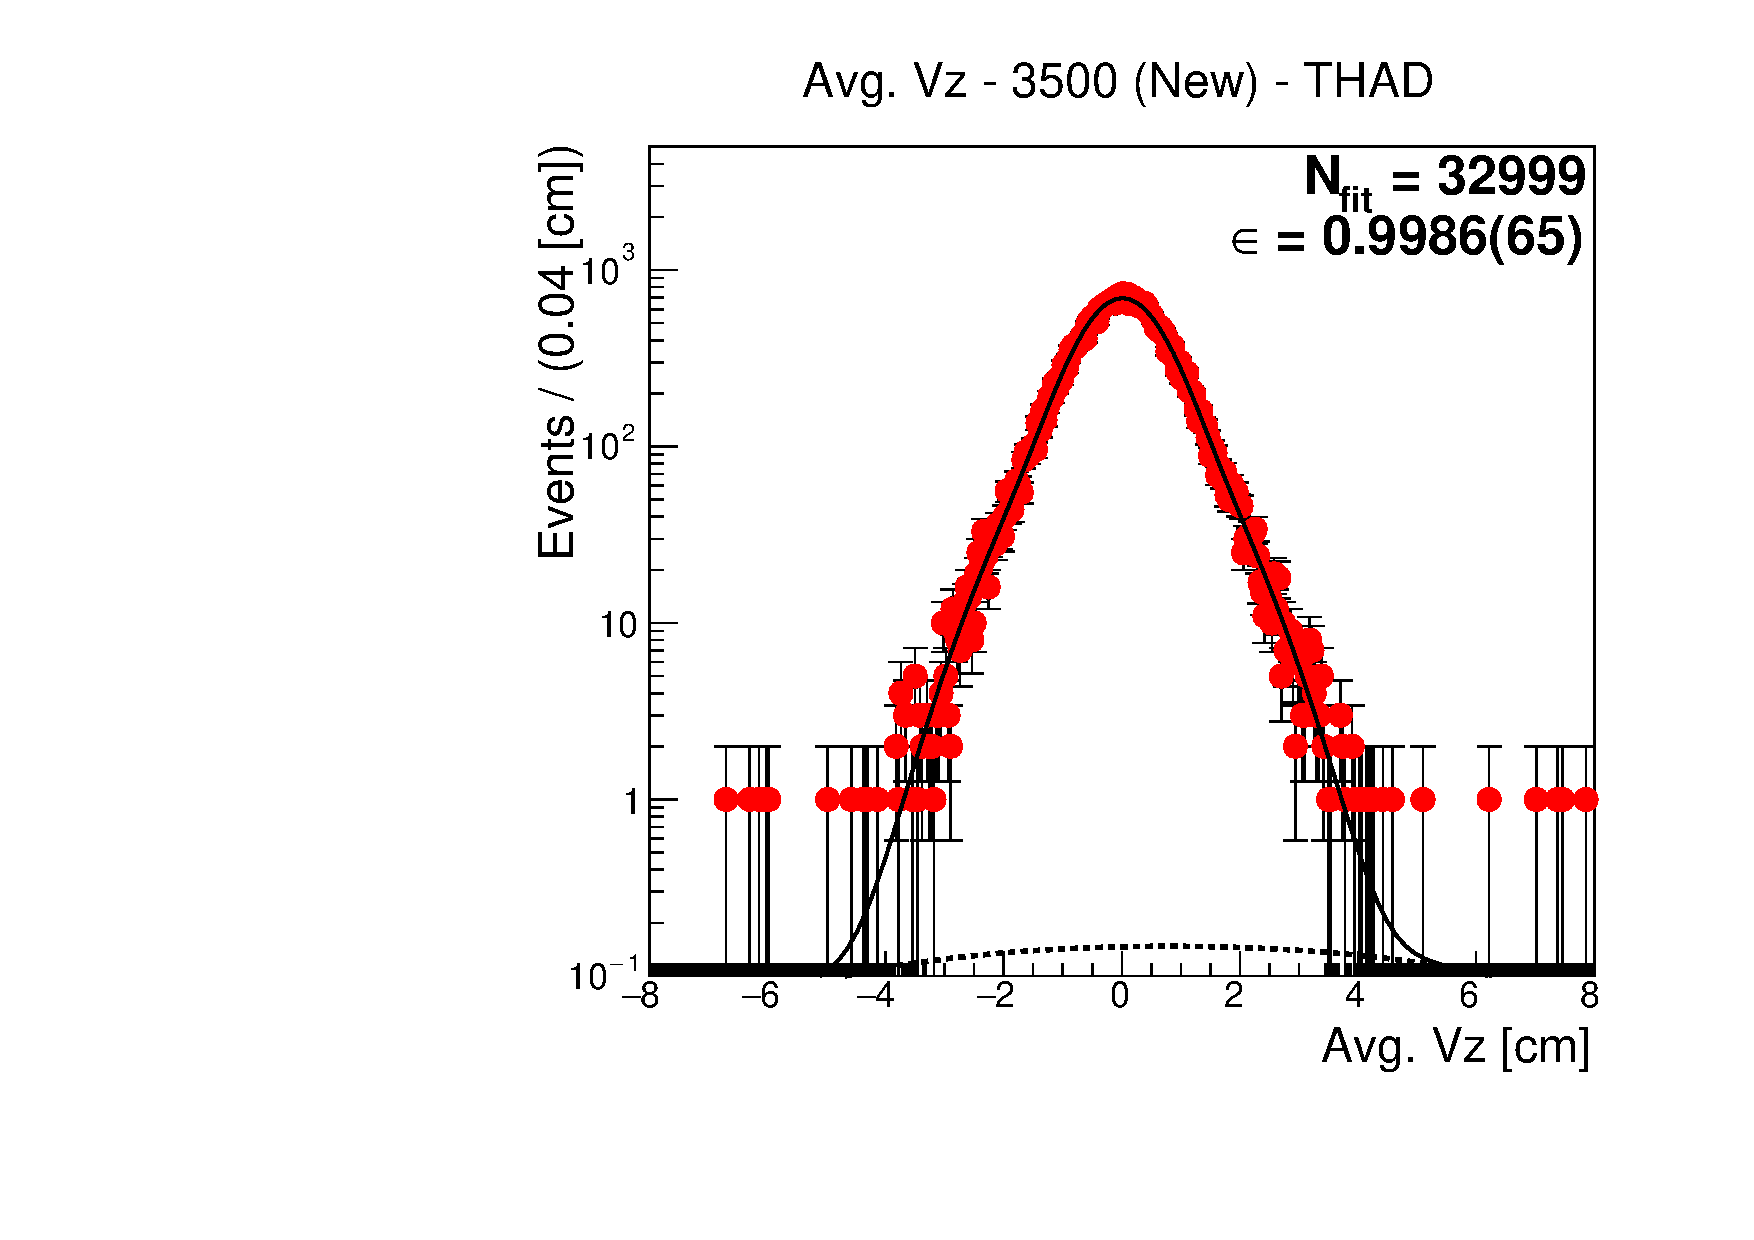
\includegraphics[scale=0.25]{figures/plots/nonDDbar_fit_results/3650_new/fit_new_3500_data_THAD.pdf}
\caption{The number of hadrons found in the 3500 (New) data sample.}
{This includes results for SHAD (left), LHAD (middle), and THAD (right).}
\label{fig:hadron_fits_3500_new}
\end{figure}

\begin{figure}[H]
\centering
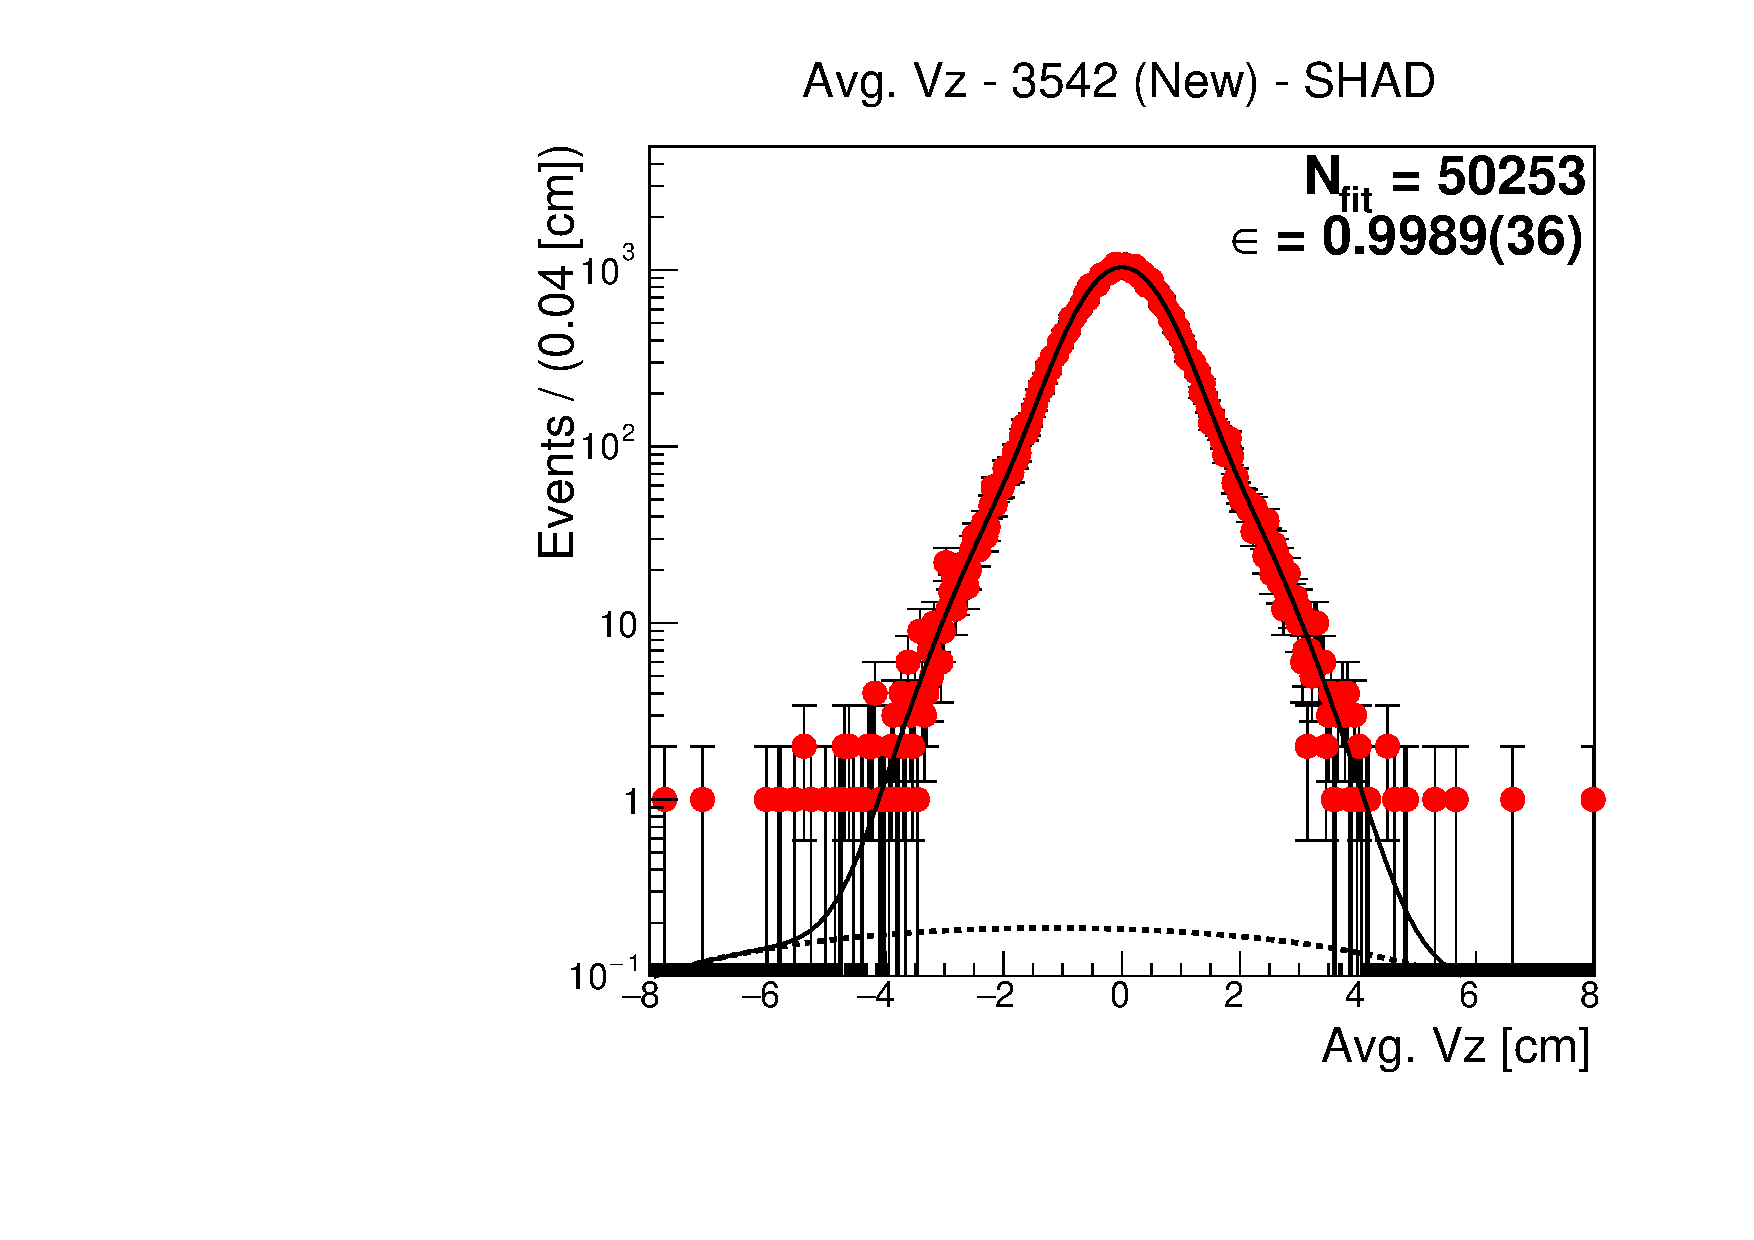
\includegraphics[scale=0.25]{figures/plots/nonDDbar_fit_results/3650_new/fit_new_3542_data_SHAD.pdf}
\hspace{-0.5cm}
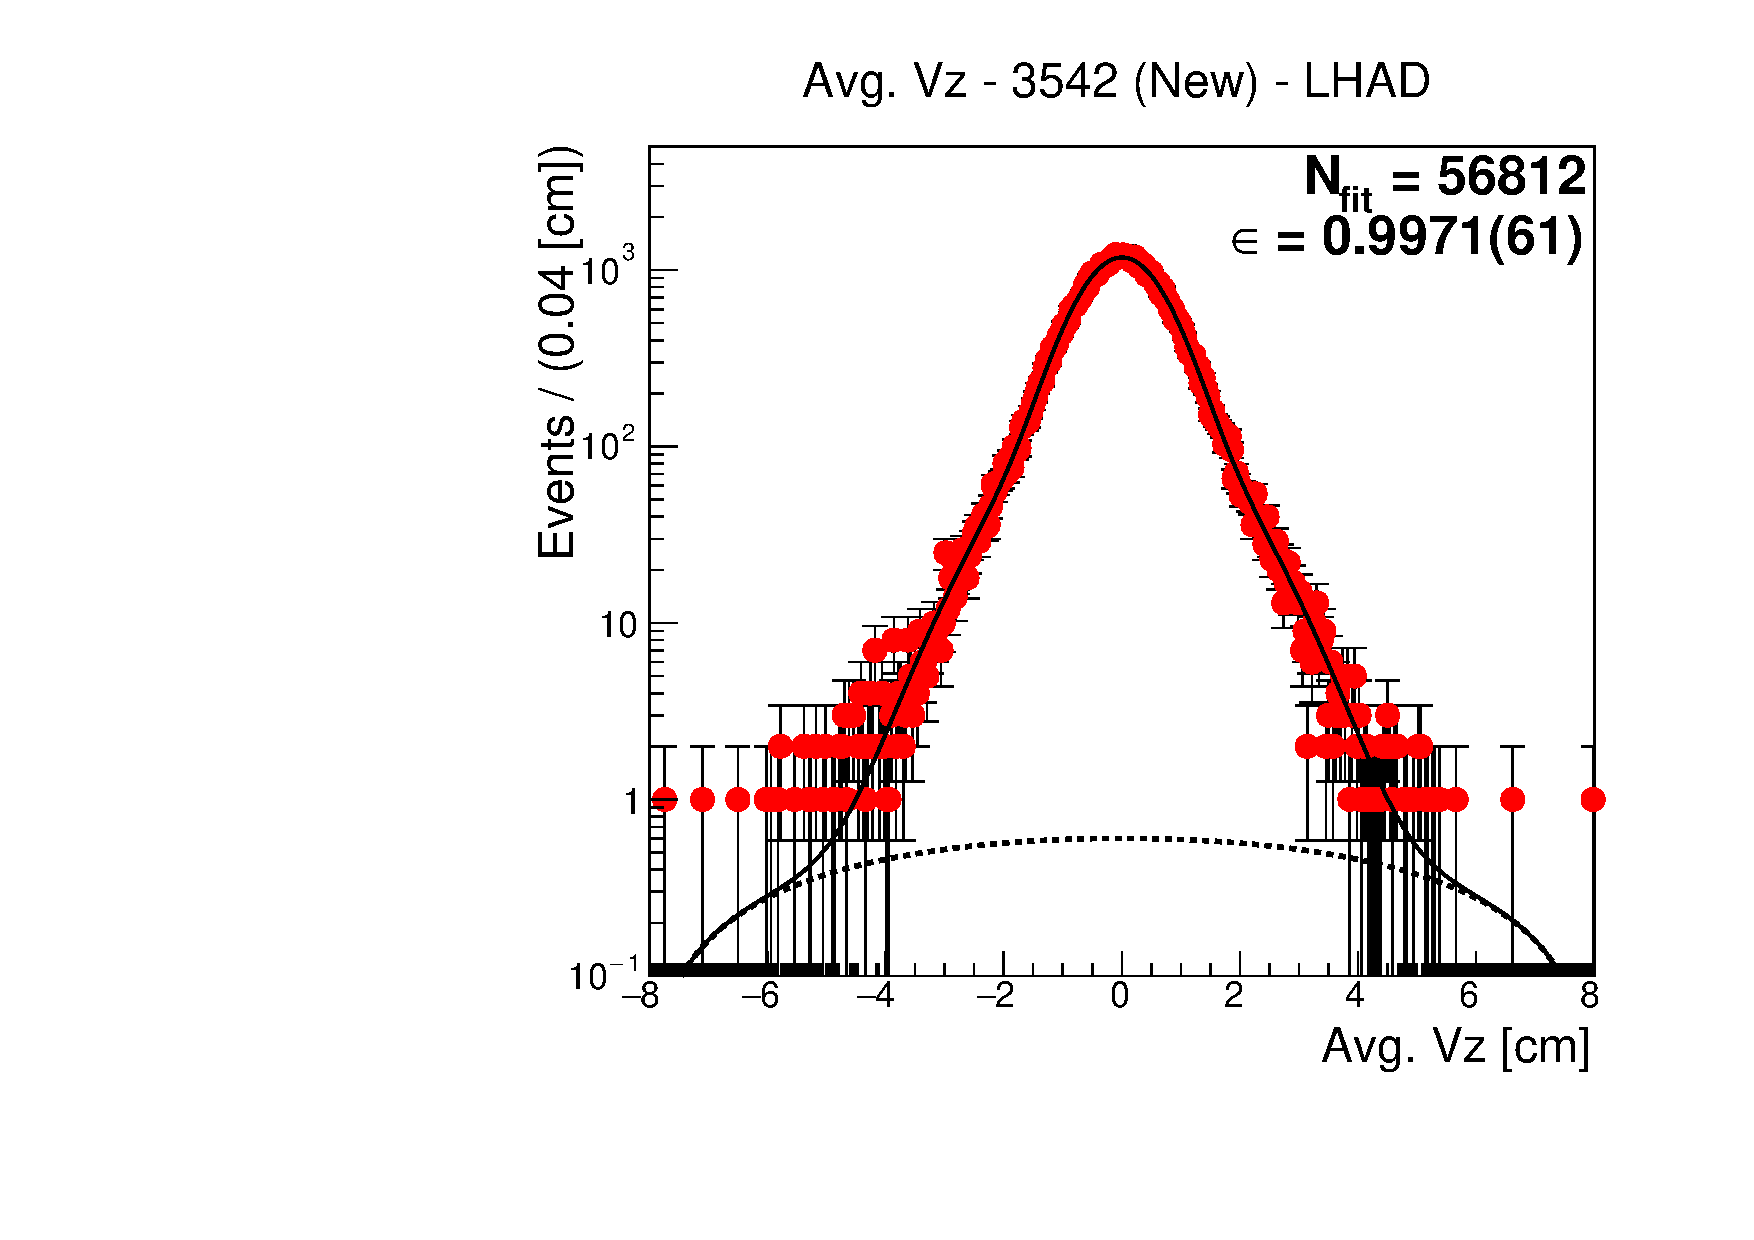
\includegraphics[scale=0.25]{figures/plots/nonDDbar_fit_results/3650_new/fit_new_3542_data_LHAD.pdf}
\hspace{-0.5cm}
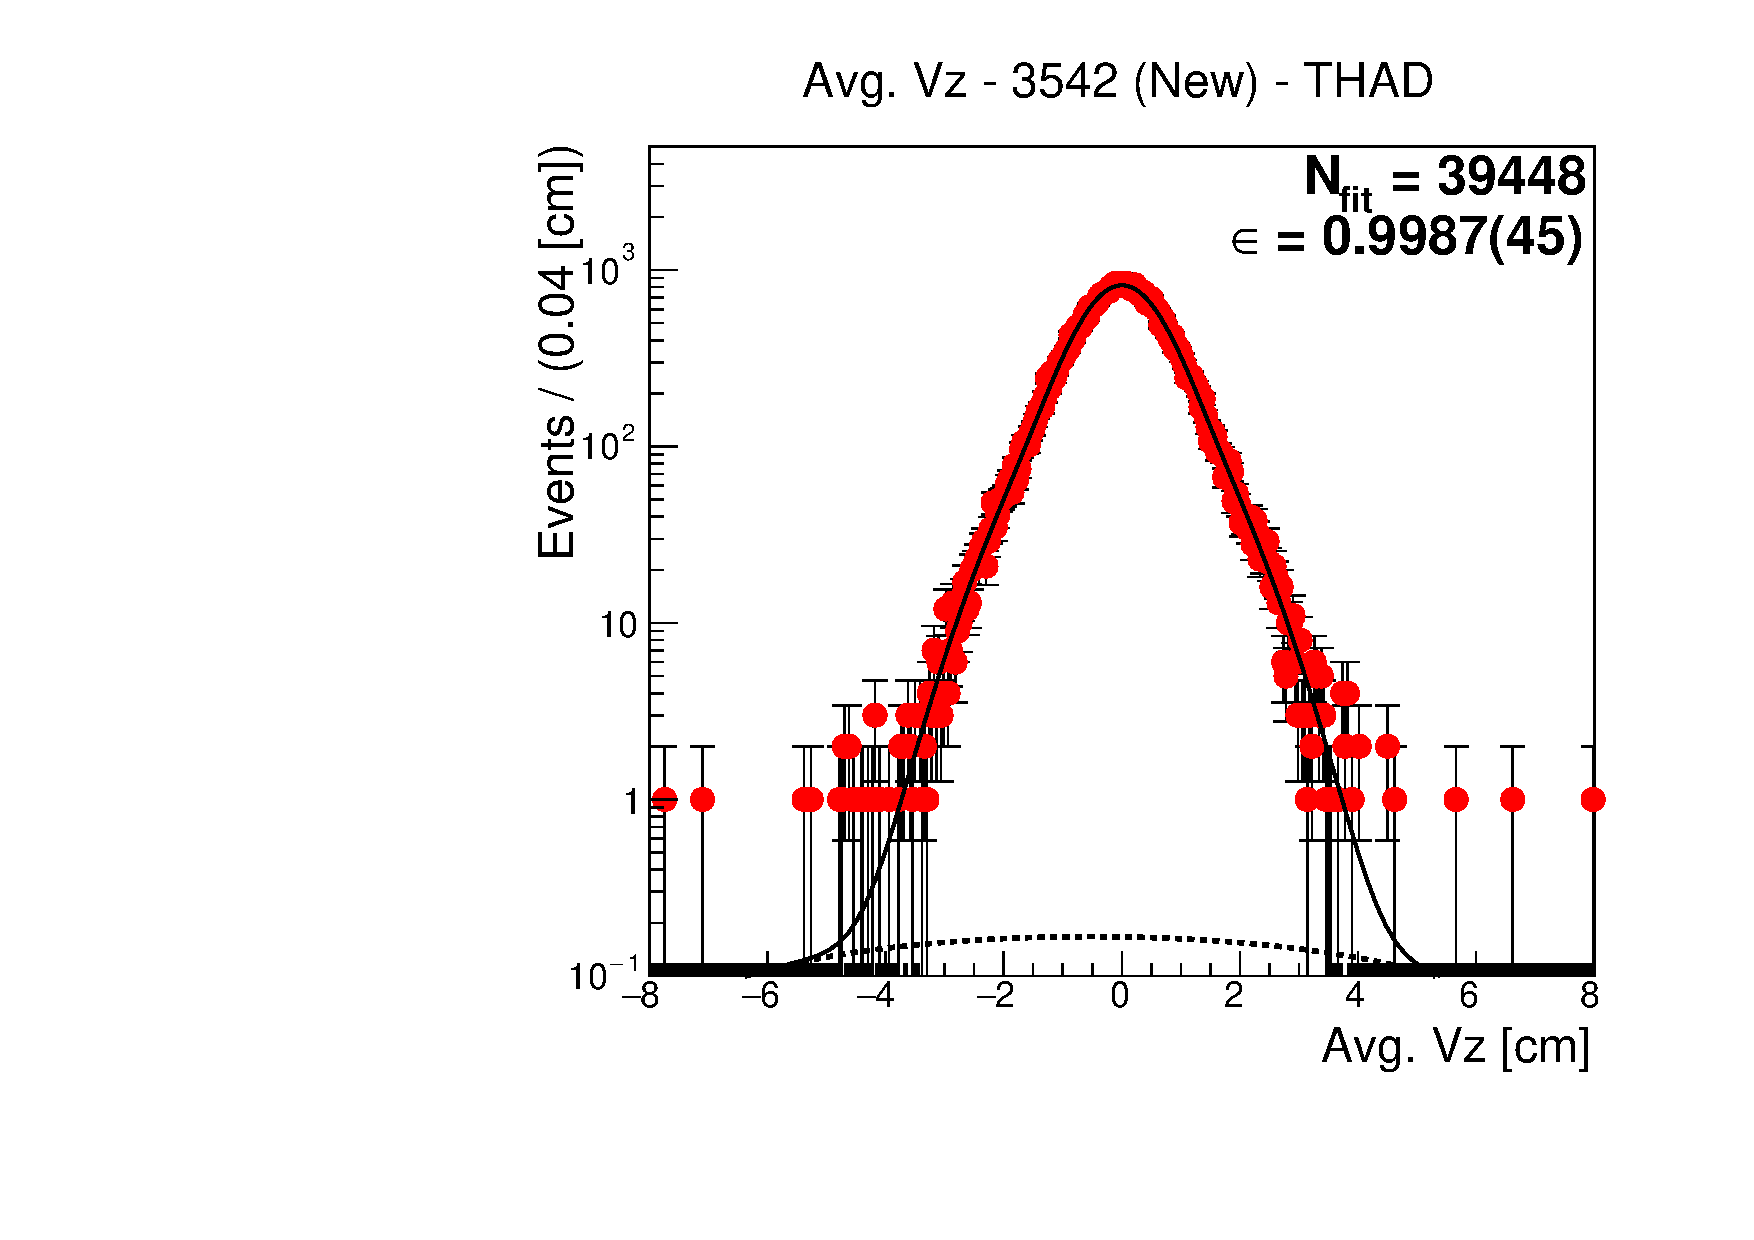
\includegraphics[scale=0.25]{figures/plots/nonDDbar_fit_results/3650_new/fit_new_3542_data_THAD.pdf}
\caption{The number of hadrons found in the 3542 (New) data sample.}
{This includes results for SHAD (left), LHAD (middle), and THAD (right).}
\label{fig:hadron_fits_3542_new}
\end{figure}


\begin{figure}[H]
\centering
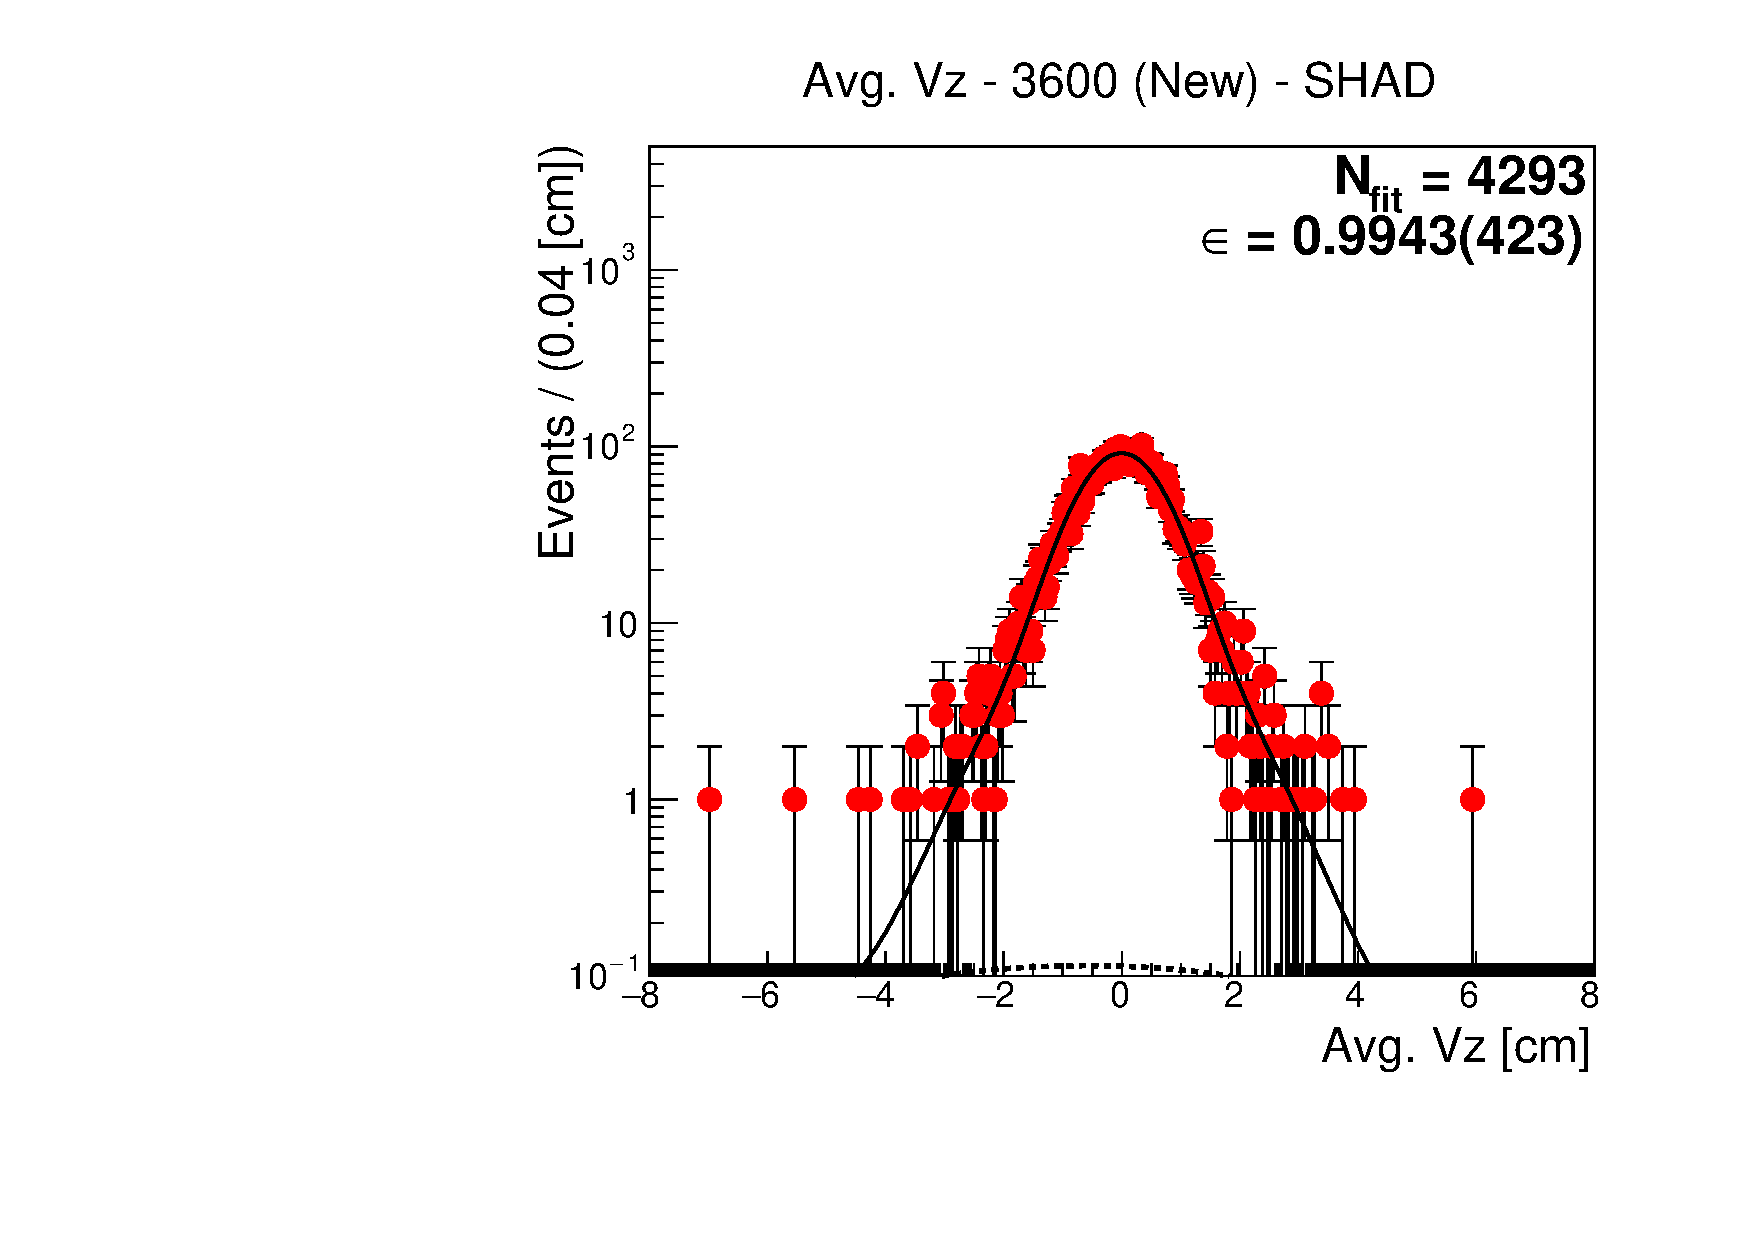
\includegraphics[scale=0.25]{figures/plots/nonDDbar_fit_results/3650_new/fit_new_3600_data_SHAD.pdf}
\hspace{-0.5cm}
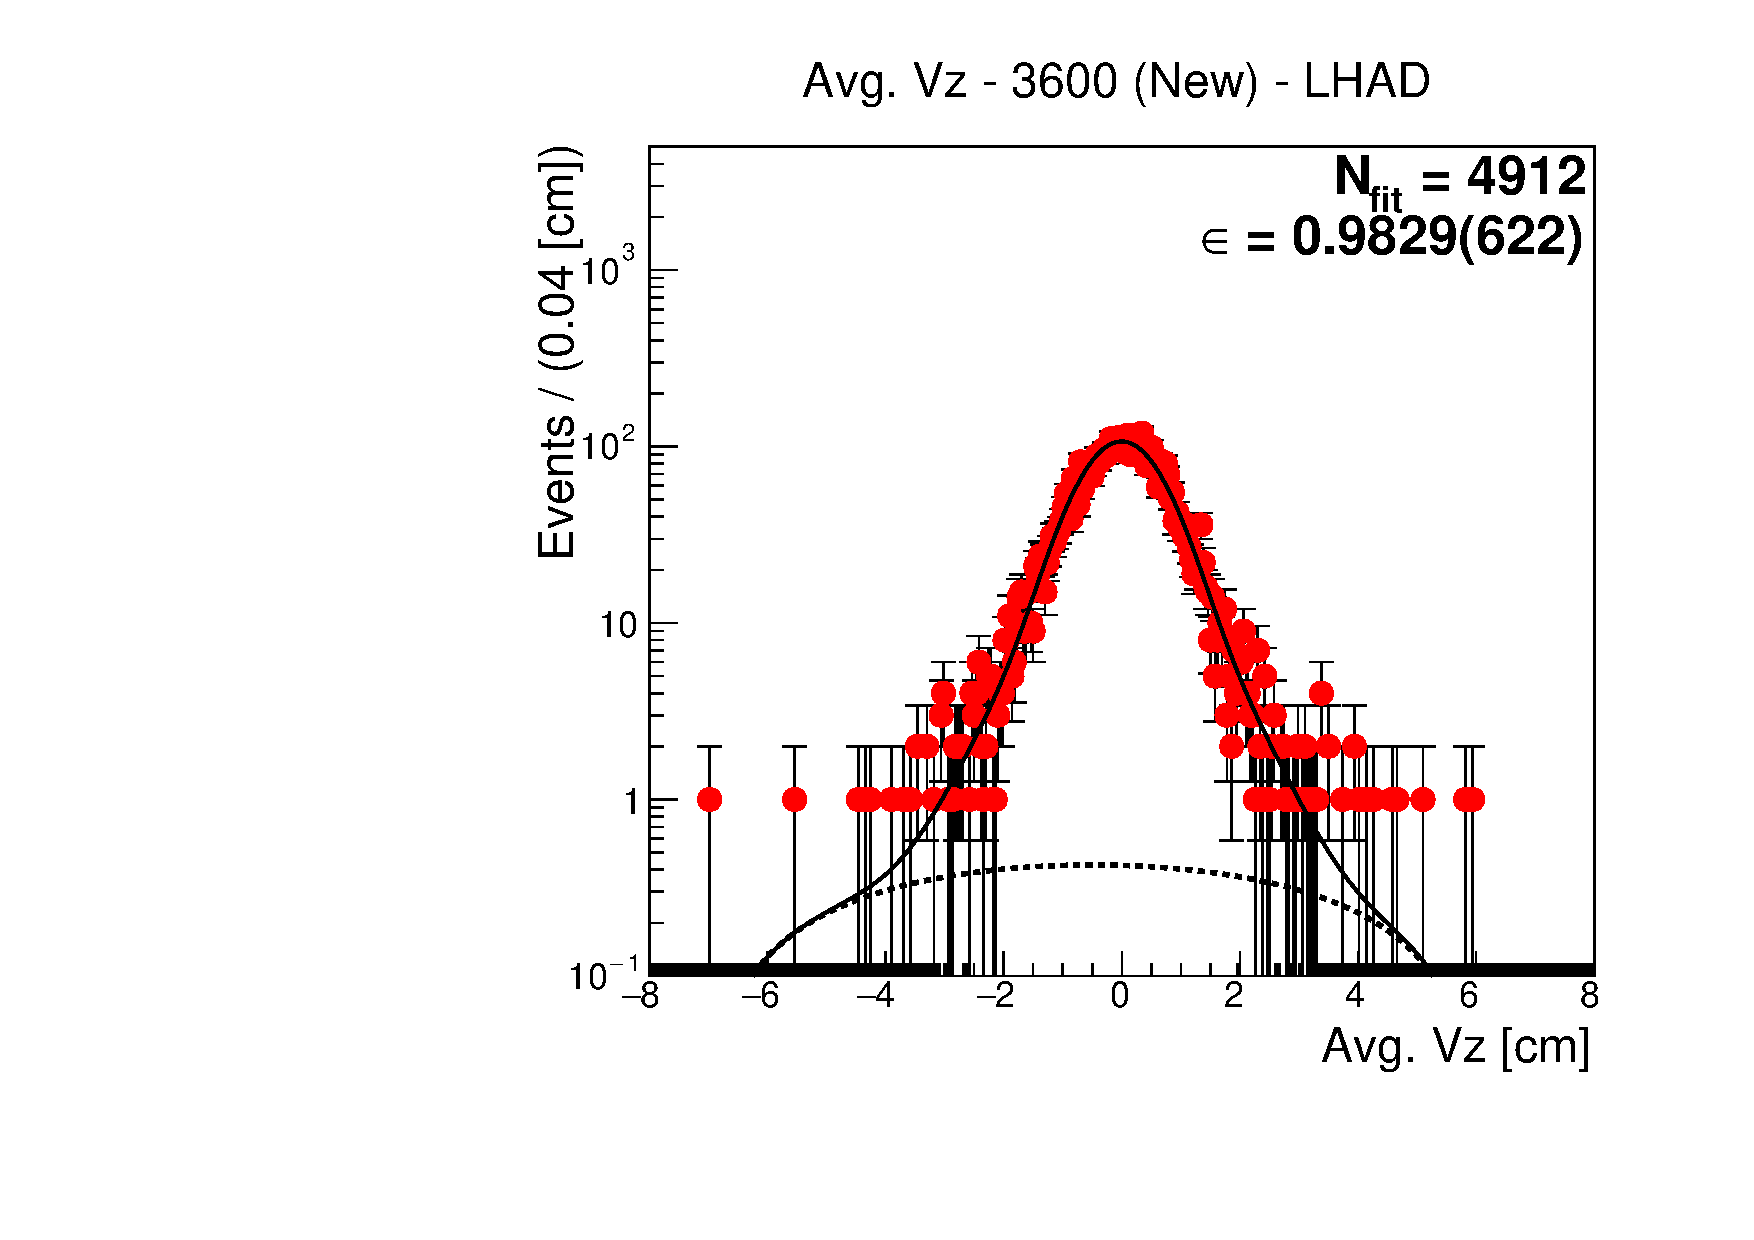
\includegraphics[scale=0.25]{figures/plots/nonDDbar_fit_results/3650_new/fit_new_3600_data_LHAD.pdf}
\hspace{-0.5cm}
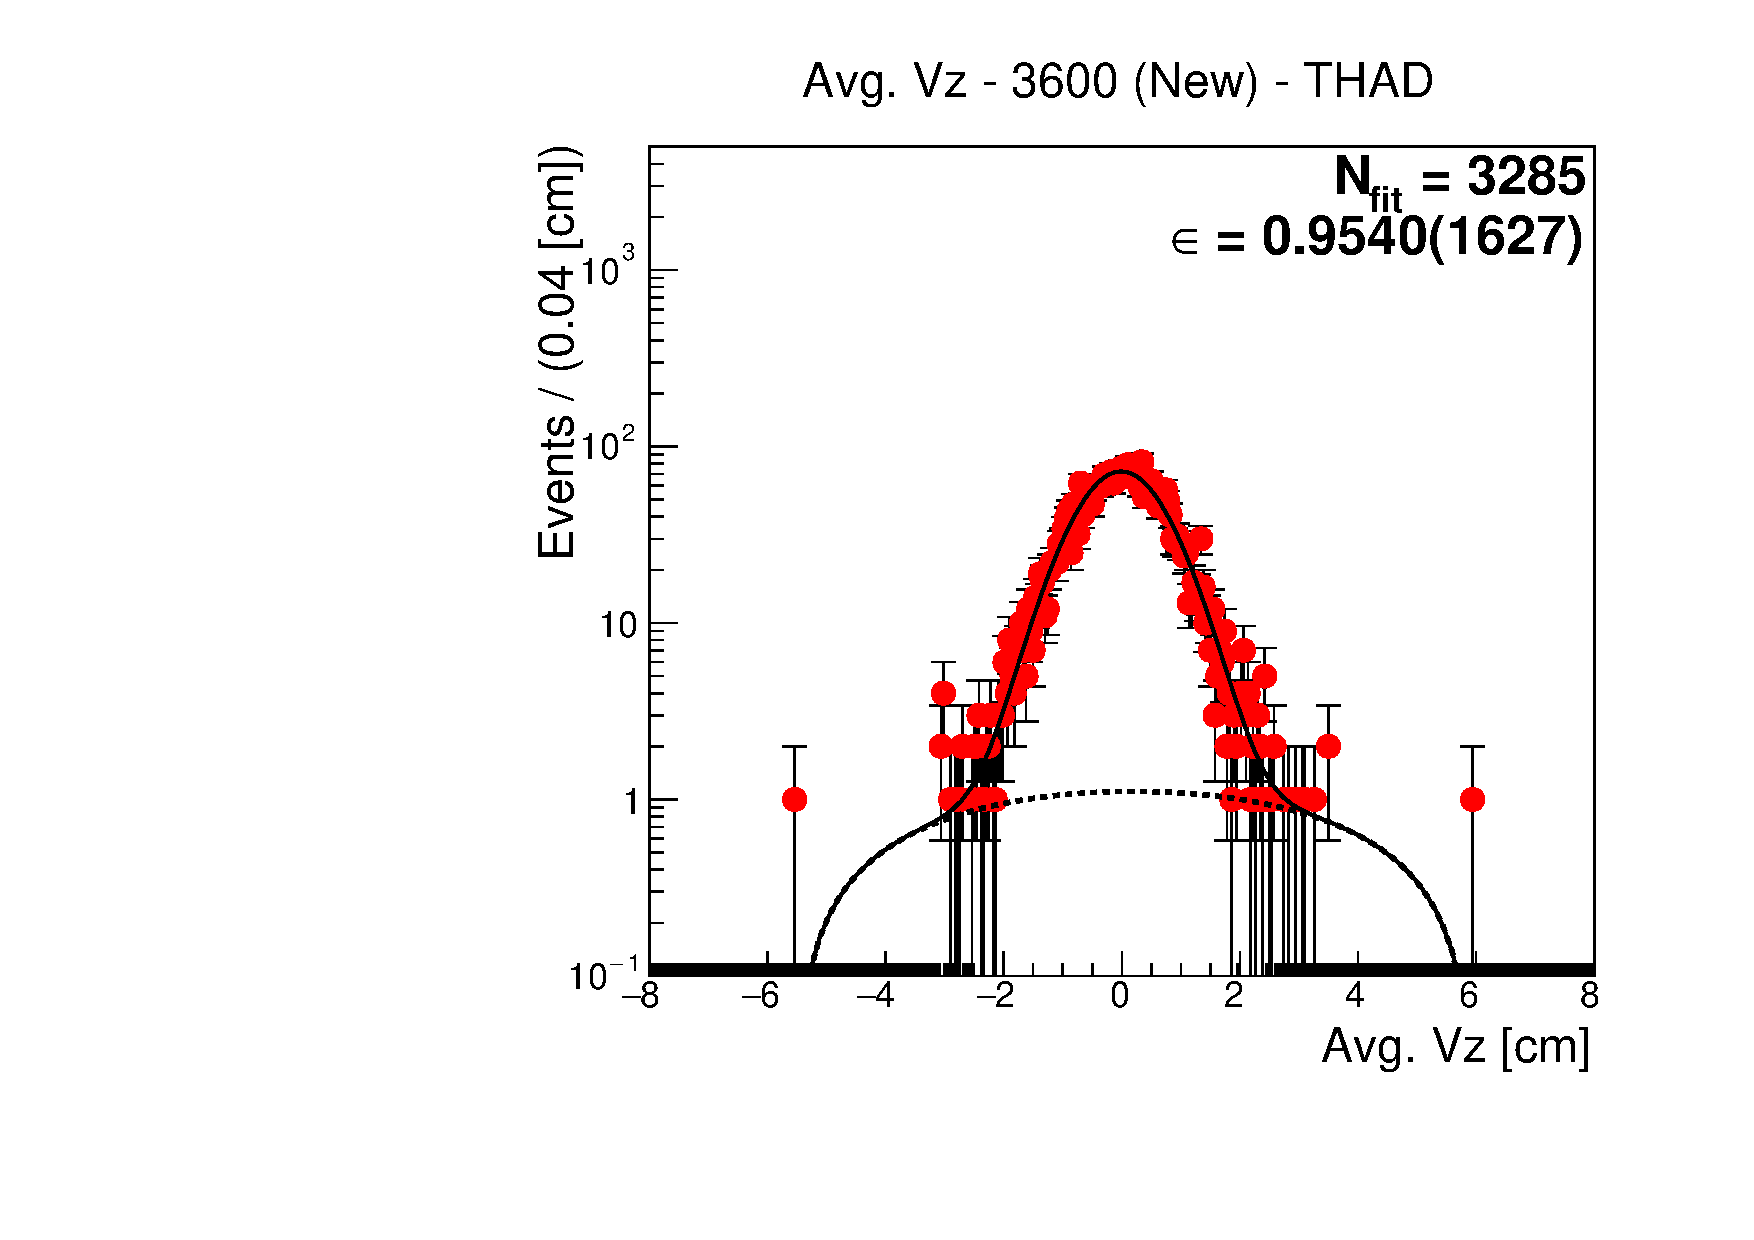
\includegraphics[scale=0.25]{figures/plots/nonDDbar_fit_results/3650_new/fit_new_3600_data_THAD.pdf}
\caption{The number of hadrons found in the 3600 (New) data sample.}
{This includes results for SHAD (left), LHAD (middle), and THAD (right).}
\label{fig:hadron_fits_3600_new}
\end{figure}


\begin{figure}[H]
\centering
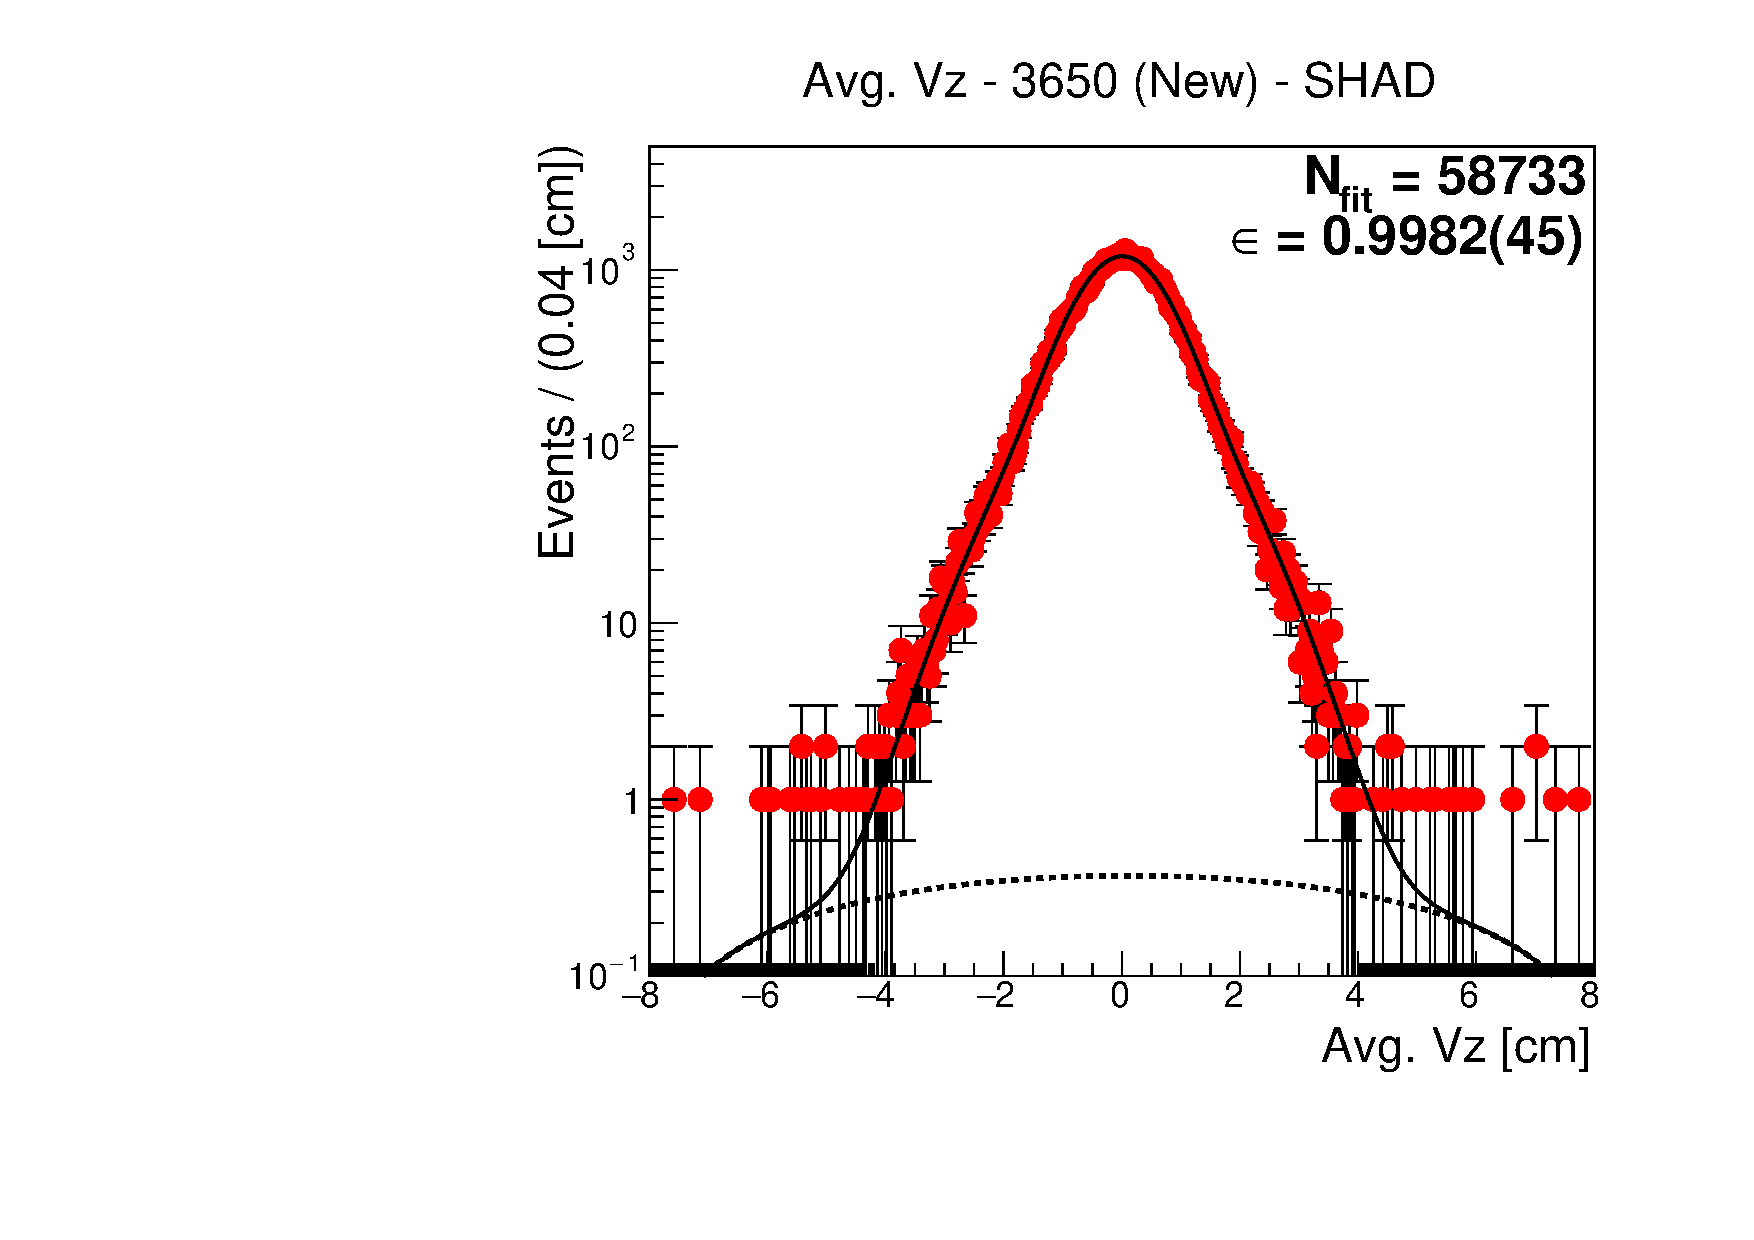
\includegraphics[scale=0.25]{figures/plots/nonDDbar_fit_results/3650_new/fit_new_3650_data_SHAD.pdf}
\hspace{-0.5cm}
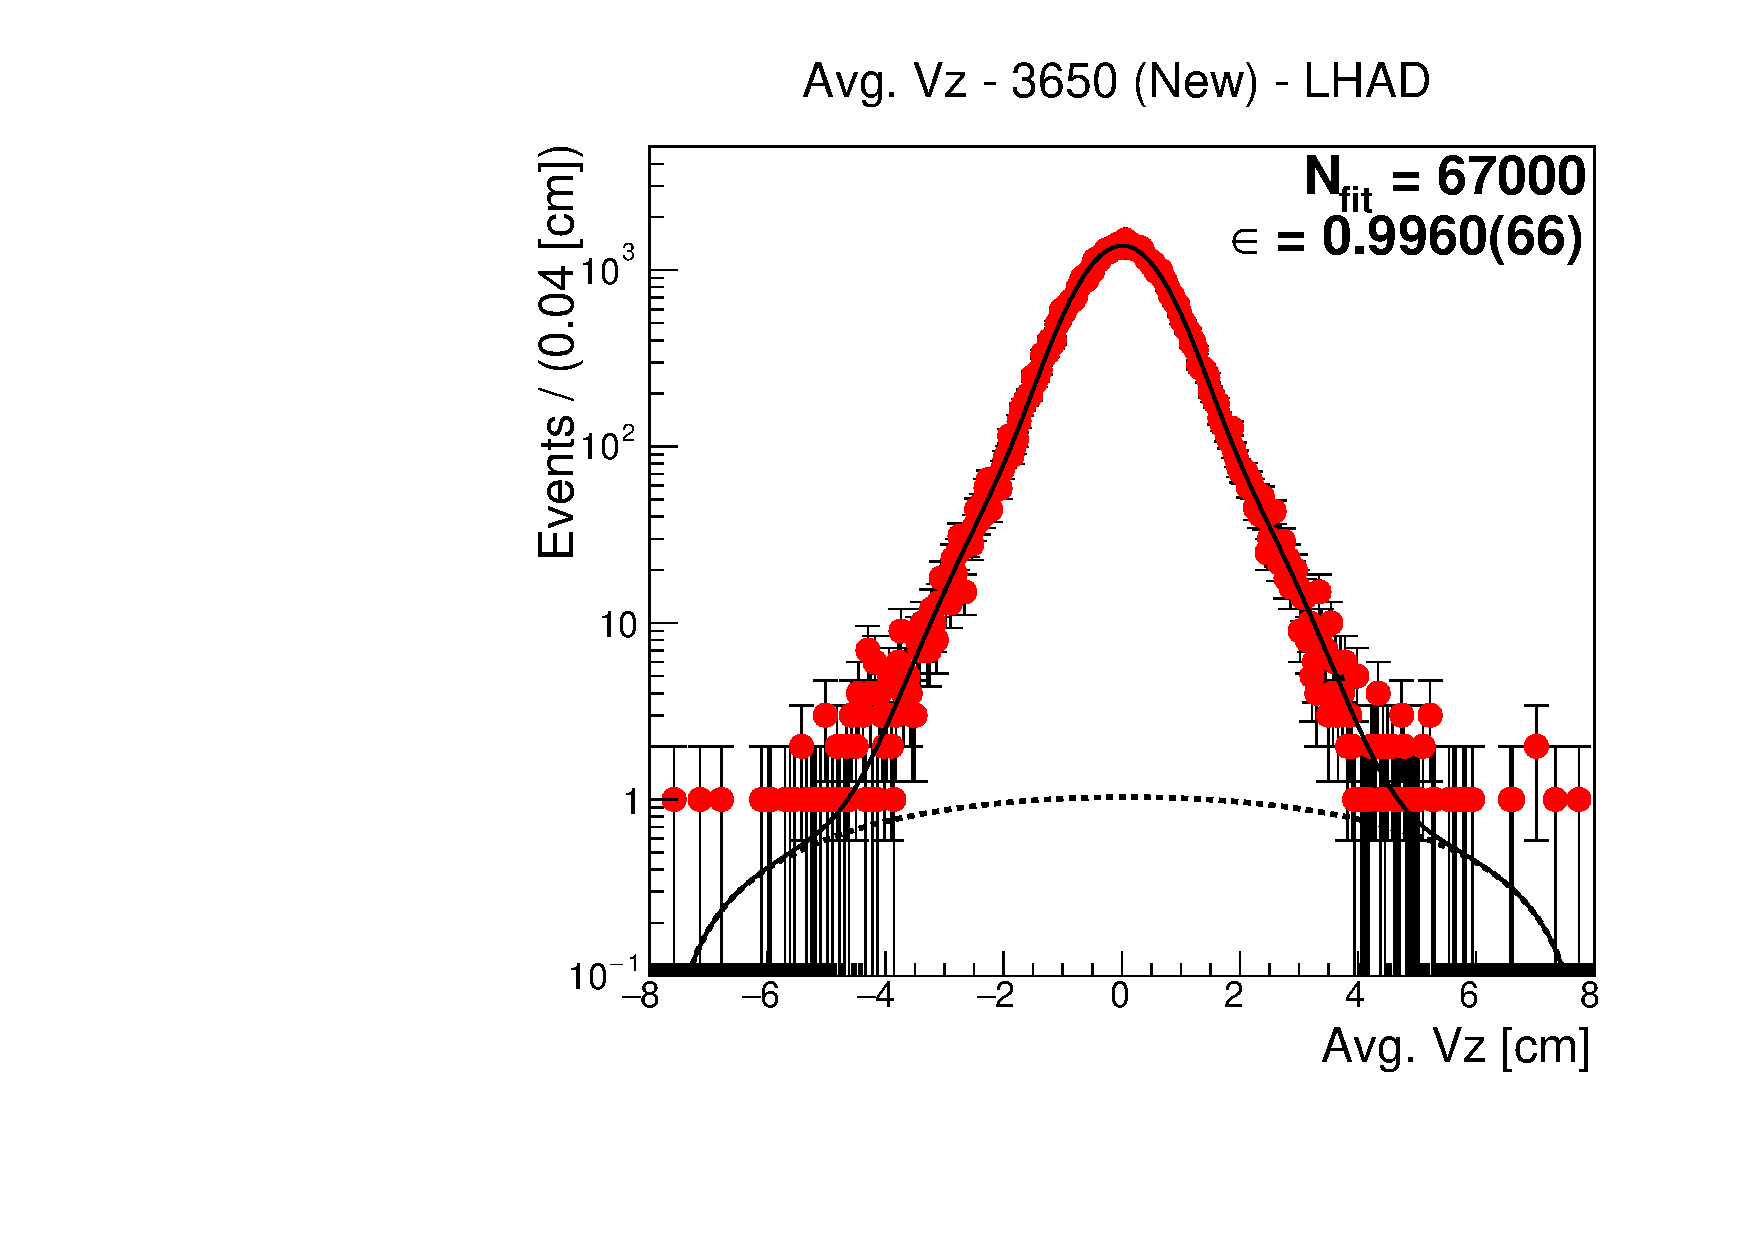
\includegraphics[scale=0.25]{figures/plots/nonDDbar_fit_results/3650_new/fit_new_3650_data_LHAD.pdf}
\hspace{-0.5cm}
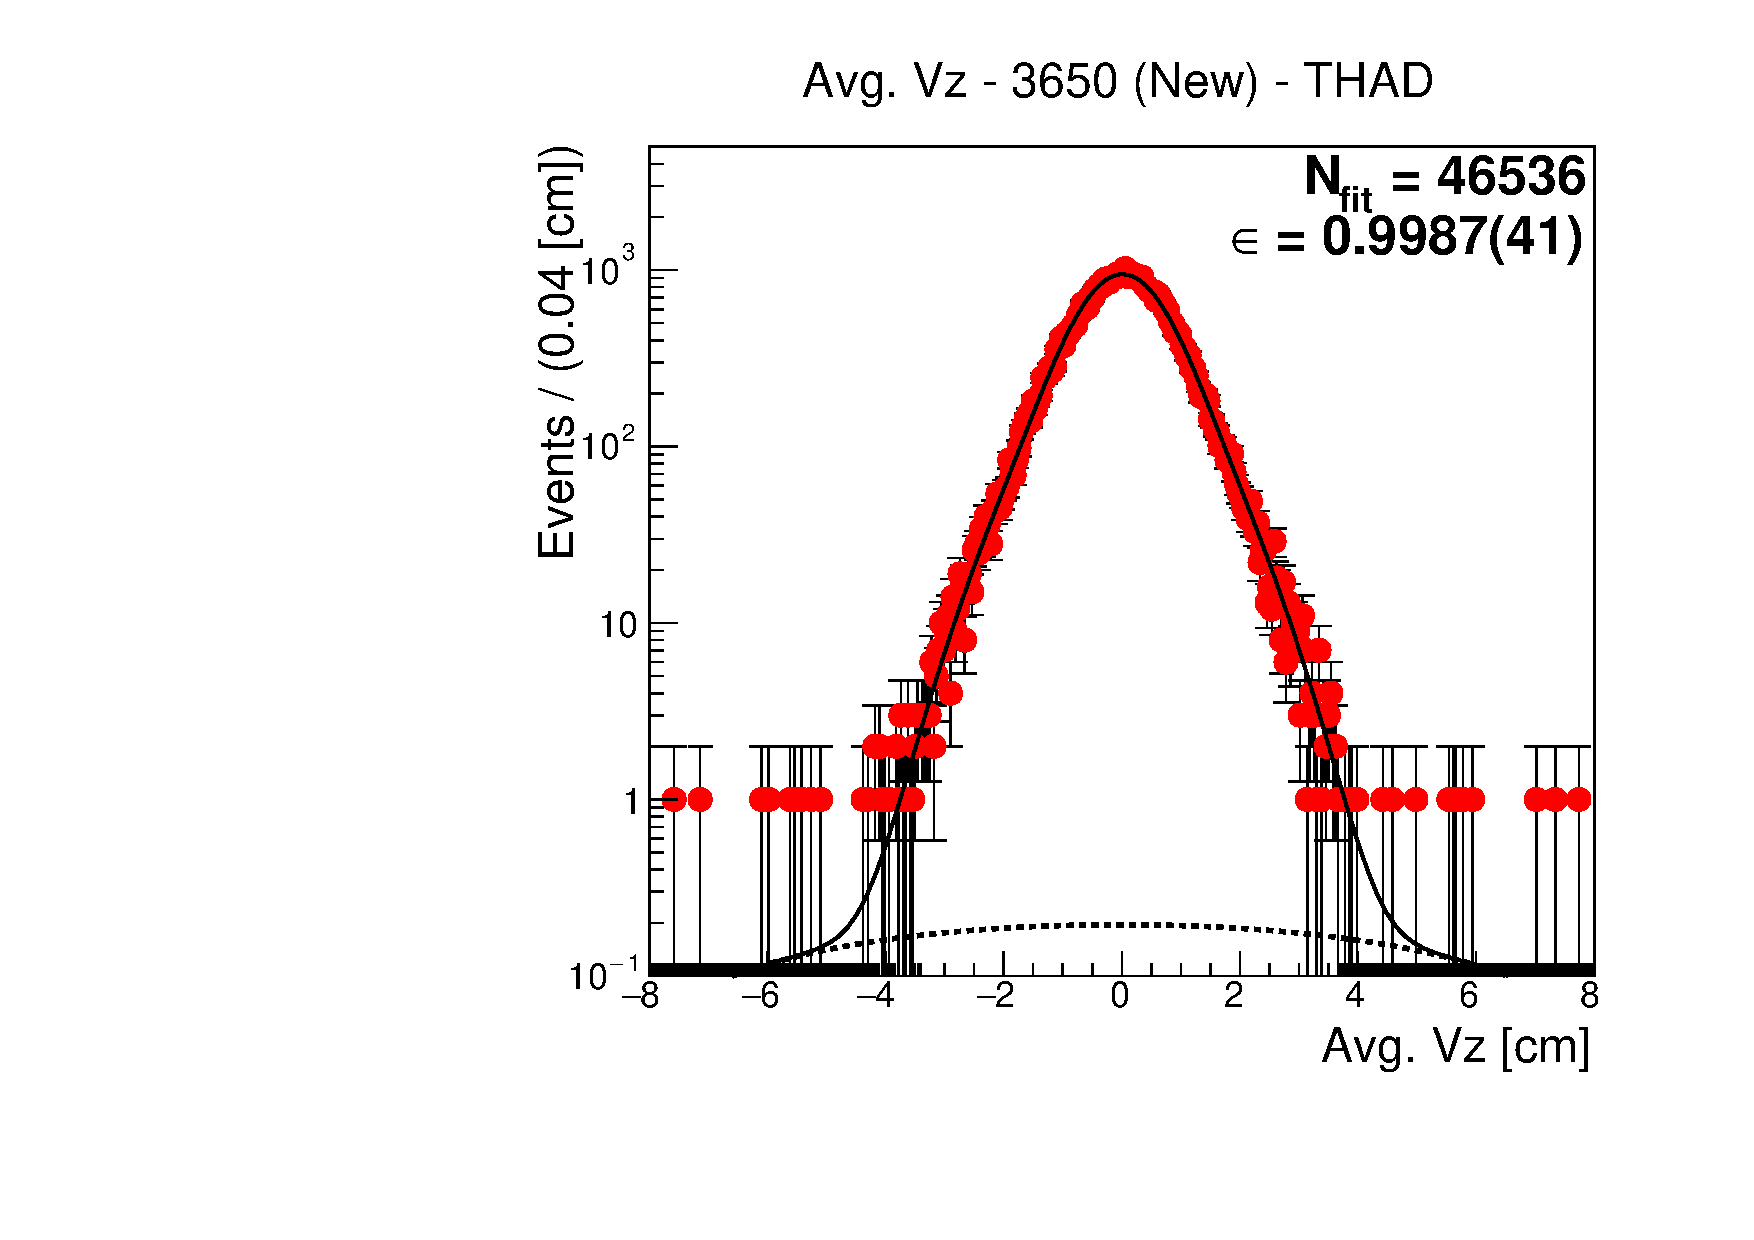
\includegraphics[scale=0.25]{figures/plots/nonDDbar_fit_results/3650_new/fit_new_3650_data_THAD.pdf}
\caption{The number of hadrons found in the 3650 (New) data sample.}
{This includes results for SHAD (left), LHAD (middle), and THAD (right).}
\label{fig:hadron_fits_3650_new}
\end{figure}


\begin{figure}[H]
\centering
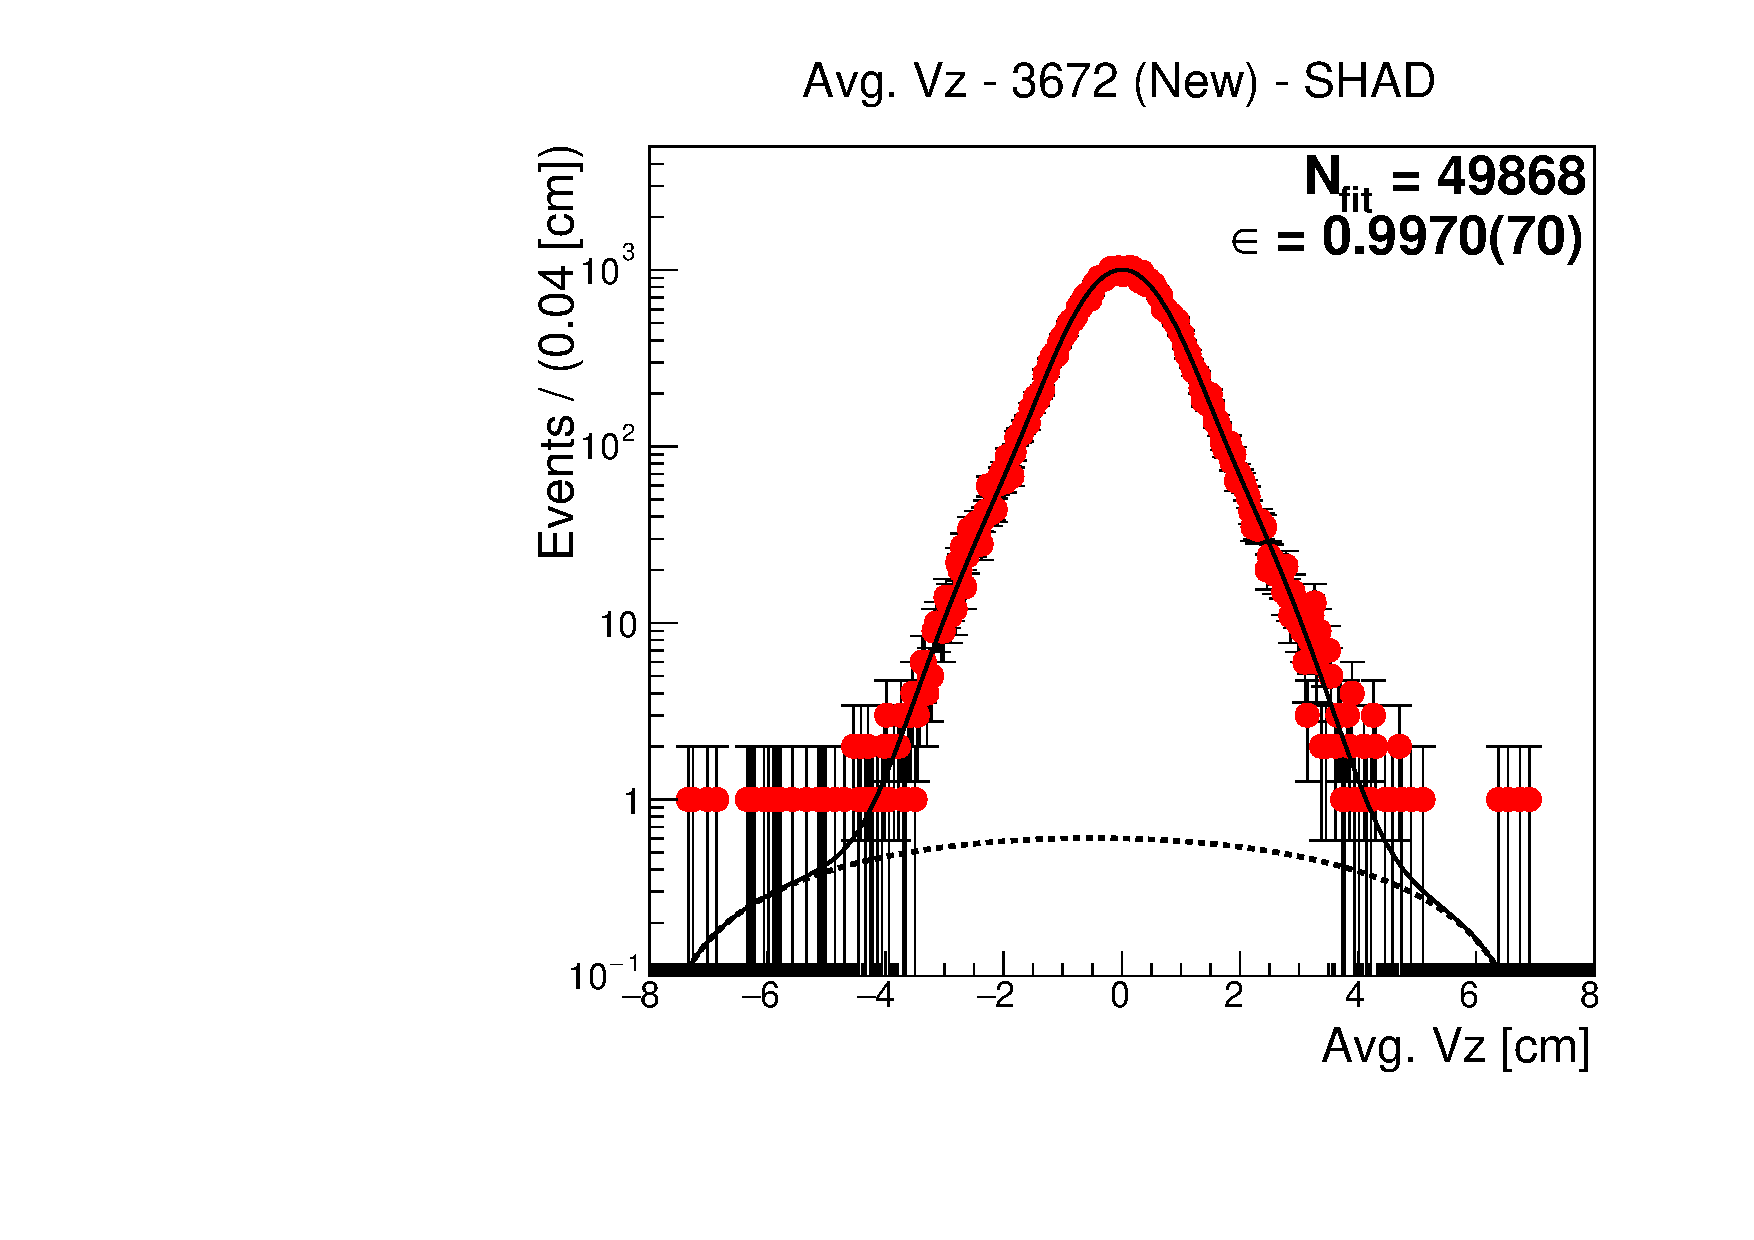
\includegraphics[scale=0.25]{figures/plots/nonDDbar_fit_results/3650_new/fit_new_3671_data_SHAD.pdf}
\hspace{-0.5cm}
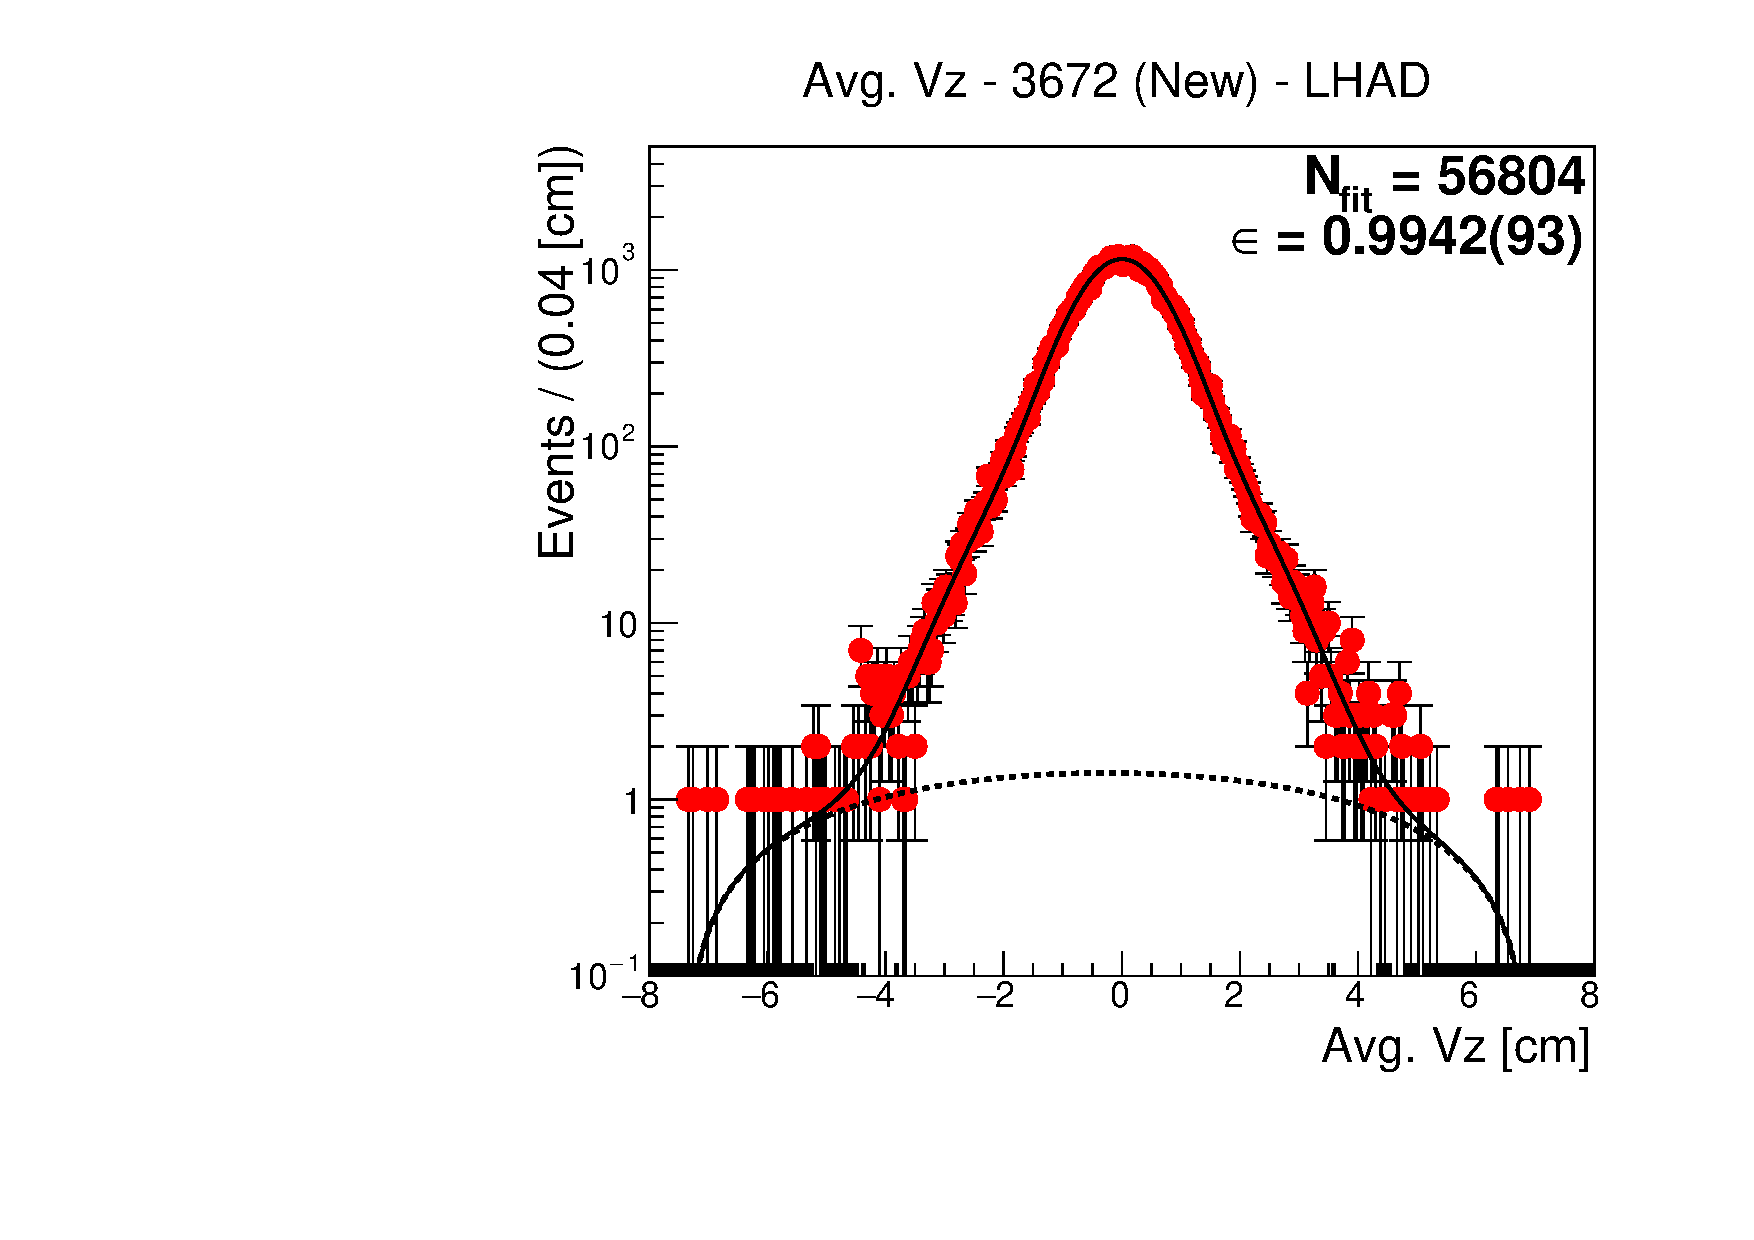
\includegraphics[scale=0.25]{figures/plots/nonDDbar_fit_results/3650_new/fit_new_3671_data_LHAD.pdf}
\hspace{-0.5cm}
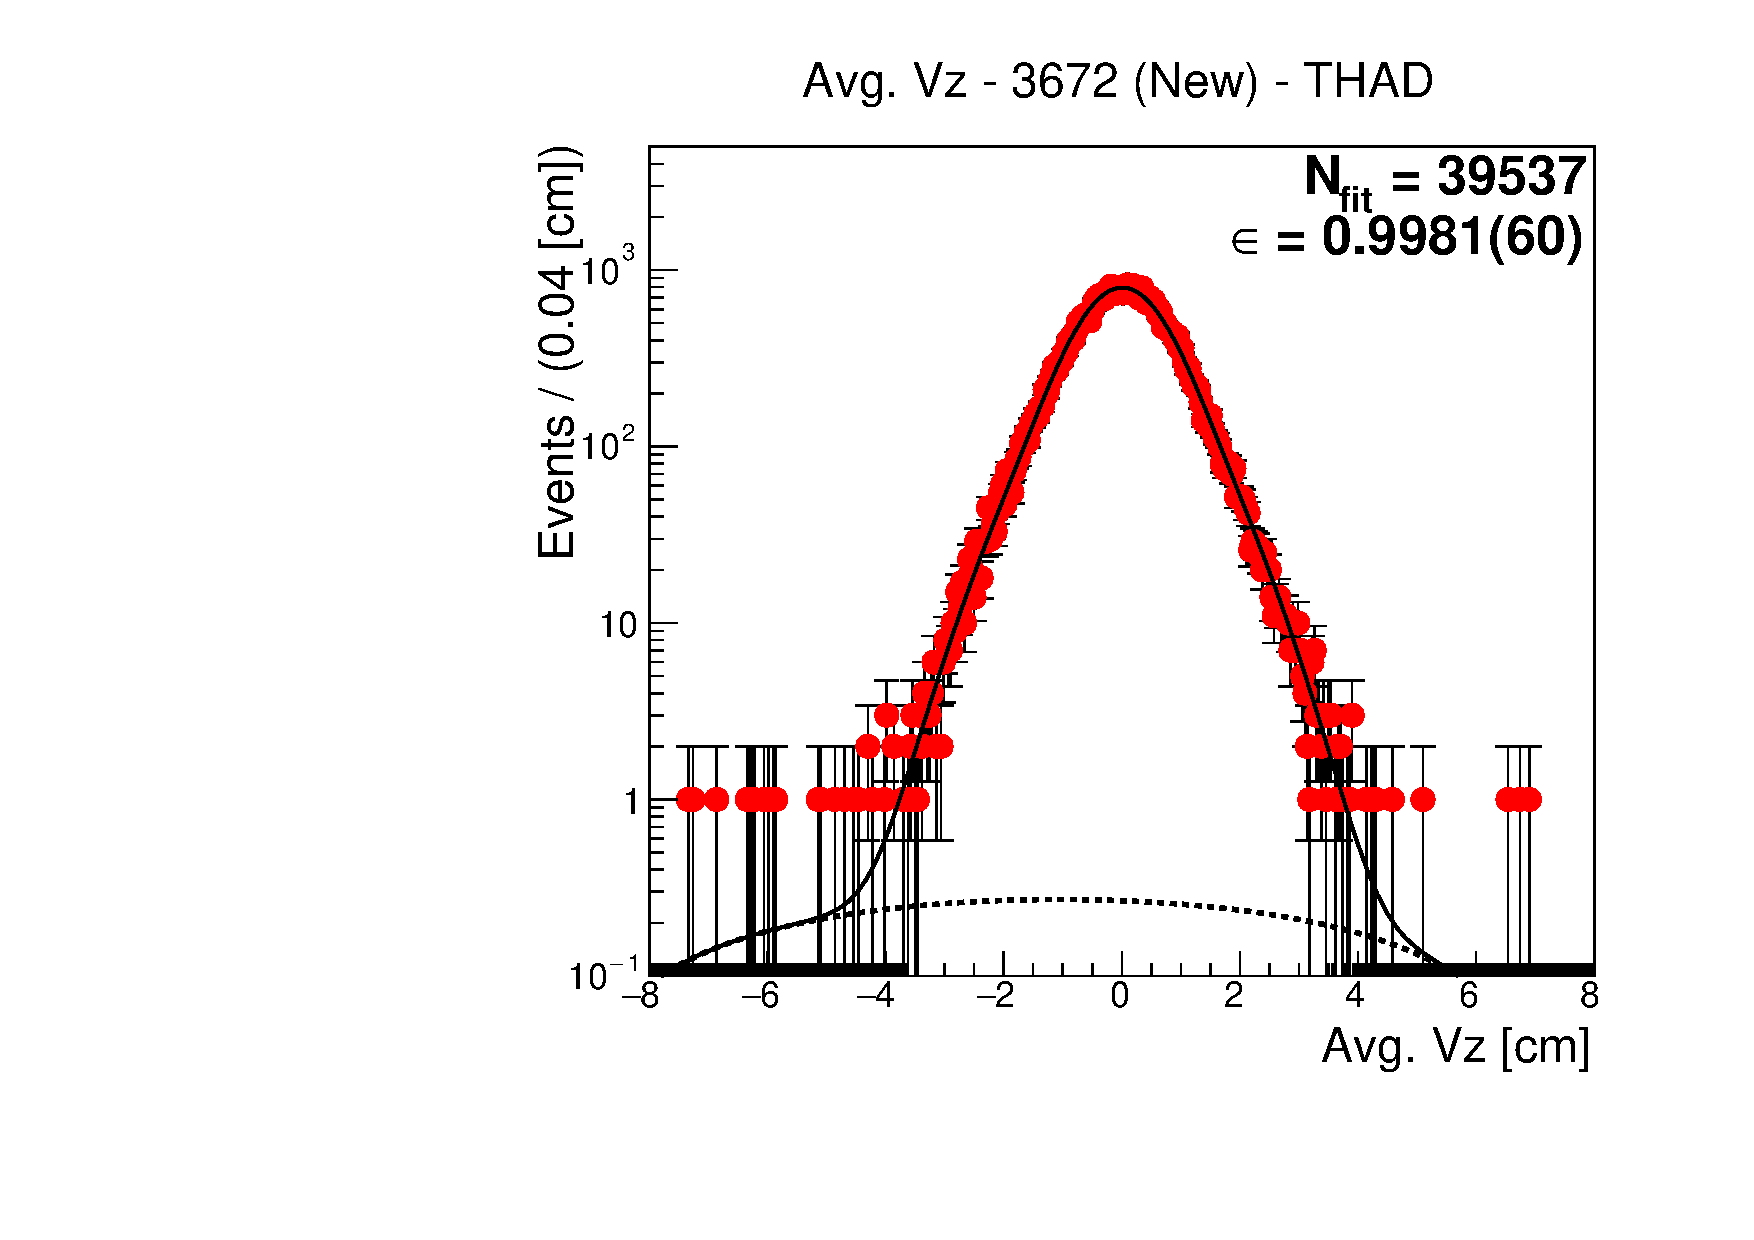
\includegraphics[scale=0.25]{figures/plots/nonDDbar_fit_results/3650_new/fit_new_3671_data_THAD.pdf}
\caption{The number of hadrons found in the 3671 (New) data sample.}
{This includes results for SHAD (left), LHAD (middle), and THAD (right).}
\label{fig:hadron_fits_3671_new}
\end{figure}



\begin{table}[H]
\centering
\renewcommand\arraystretch{1.0}

\begin{tabular}{c|r|cr@{$\; \pm \;$}rc cr@{$\; \pm \;$}rc cr@{$\; \pm \;$}rc}
\hline
\multicolumn{14}{c}{3500 (New) Reconstruction} \\
\hline
Sample & $\sigma$ [\si{\nb}] & \multicolumn{4}{c}{$\effmc$ (SHAD) [\%]} & \multicolumn{4}{c}{$\effmc$ (LHAD) [\%]} & \multicolumn{4}{c}{$\effmc$ (THAD) [\%]} \\
\hline
$\tautau$       & 0.000 && \mcd{2}         &&& \mcd{2}         &&& \mcd{2}         & \\
$\yjpsi$        & 1.831 &&  47.079 & 0.077 &&&  56.117 & 0.084 &&&  35.320 & 0.066 & \\
$\twophoton$    & 1.240 &&   2.380 & 0.017 &&&   4.924 & 0.025 &&&   1.644 & 0.014 & \\
$\psip^\dagger$ & 0.006 &&  62.989 & 0.008 &&&  69.288 & 0.008 &&&  51.694 & 0.007 & \\
\hline          
\end{tabular}

\vspace{0.5cm}

\begin{tabular}{c|r|cr@{$\; \pm \;$}rc cr@{$\; \pm \;$}rc cr@{$\; \pm \;$}rc}
\hline
\multicolumn{14}{c}{3542 (New) Reconstruction} \\
\hline
Sample & $\sigma$ [\si{\nb}] & \multicolumn{4}{c}{$\effmc$ (SHAD) [\%]} & \multicolumn{4}{c}{$\effmc$ (LHAD) [\%]} & \multicolumn{4}{c}{$\effmc$ (THAD) [\%]} \\
\hline
$\tautau$       & 0.000 && \mcd{2}        &&& \mcd{2}        &&& \mcd{2}        & \\
$\yjpsi$        & 1.632 && 47.188 & 0.072 &&& 56.430 & 0.079 &&& 35.355 & 0.063 & \\
$\twophoton$    & 1.270 &&  2.386 & 0.016 &&&  5.046 & 0.024 &&&  1.633 & 0.013 & \\
$\psip^\dagger$ & 0.009 && 62.989 & 0.008 &&& 69.288 & 0.008 &&& 51.694 & 0.007 & \\
\hline          
\end{tabular}

\vspace{0.5cm}

\begin{tabular}{c|r|cr@{$\; \pm \;$}rc cr@{$\; \pm \;$}rc cr@{$\; \pm \;$}rc}
\hline
\multicolumn{14}{c}{3600 (New) Reconstruction} \\
\hline
Sample & $\sigma$ [\si{\nb}] & \multicolumn{4}{c}{$\effmc$ (SHAD) [\%]} & \multicolumn{4}{c}{$\effmc$ (LHAD) [\%]} & \multicolumn{4}{c}{$\effmc$ (THAD) [\%]} \\
\hline
$\tautau$       & 1.262 && 12.851 & 0.080 &&& 29.096 & 0.121 &&& 10.040 & 0.071 & \\
$\yjpsi$        & 1.412 && 47.524 & 0.154 &&& 56.902 & 0.169 &&& 35.703 & 0.134 & \\
$\twophoton$    & 1.311 &&  2.651 & 0.036 &&&  5.089 & 0.050 &&&  1.897 & 0.031 & \\
$\psip^\dagger$ & 0.024 && 62.989 & 0.008 &&& 69.288 & 0.008 &&& 51.694 & 0.007 & \\
\hline          
\end{tabular}

\vspace{0.5cm}

\begin{tabular}{c|r|cr@{$\; \pm \;$}rc cr@{$\; \pm \;$}rc cr@{$\; \pm \;$}rc}
\hline
\multicolumn{14}{c}{3650 (New) Reconstruction} \\
\hline
Sample & $\sigma$ [\si{\nb}] & \multicolumn{4}{c}{$\effmc$ (SHAD) [\%]} & \multicolumn{4}{c}{$\effmc$ (LHAD) [\%]} & \multicolumn{4}{c}{$\effmc$ (THAD) [\%]} \\
\hline
$\tautau$       & 1.844 && 12.964 & 0.033 &&& 28.939 & 0.049 &&& 10.154 & 0.029 & \\
$\yjpsi$        & 1.260 && 47.414 & 0.063 &&& 57.043 & 0.069 &&& 35.701 & 0.055 & \\
$\twophoton$    & 1.346 &&  2.410 & 0.014 &&&  4.675 & 0.020 &&&  1.682 & 0.012 & \\
$\psip^\dagger$ & 0.110 && 62.989 & 0.008 &&& 69.288 & 0.008 &&& 51.694 & 0.007 & \\
\hline          
\end{tabular}

\vspace{0.5cm}

\begin{tabular}{c|r|cr@{$\; \pm \;$}rc cr@{$\; \pm \;$}rc cr@{$\; \pm \;$}rc}
\hline
\multicolumn{14}{c}{3671 (New) Reconstruction} \\
\hline
Sample & $\sigma$ [\si{\nb}] & \multicolumn{4}{c}{$\effmc$ (SHAD) [\%]} & \multicolumn{4}{c}{$\effmc$ (LHAD) [\%]} & \multicolumn{4}{c}{$\effmc$ (THAD) [\%]} \\
\hline
$\tautau$       & 2.026 && 12.997 & 0.047 &&& 28.851 & 0.069 &&& 10.169 & 0.041 & \\
$\yjpsi$        & 1.205 && 47.496 & 0.089 &&& 57.237 & 0.098 &&& 35.745 & 0.077 & \\
$\twophoton$    & 1.361 &&  2.473 & 0.020 &&&  4.787 & 0.028 &&&  1.698 & 0.017 & \\
$\psip^\dagger$ & 0.436 && 62.989 & 0.008 &&& 69.288 & 0.008 &&& 51.694 & 0.007 & \\
\hline          
\end{tabular}

\caption{Reconstruction of background samples for the new continuum data.}
{$^\dagger$ The $\psip$ is assumed to have a standard Breit-Wigner shape.}
\label{tab:3650_new_reconstruction}
\end{table}

\begin{table}[H]
\centering
\renewcommand\arraystretch{1.0}

\begin{tabular}{c|cr@{$\; \pm \;$}rc cr@{$\; \pm \;$}rc cr@{$\; \pm \;$}rc}
\hline
\multicolumn{13}{c}{3500 (New) Results} \\
\hline
Sample         & \multicolumn{4}{c}{$\Nhad$ (SHAD)} & \multicolumn{4}{c}{$\Nhad$ (LHAD)} & \multicolumn{4}{c}{$\Nhad$ (THAD)} \\
\hline
Data            && 42106 & 205 &&& 47942 & 219 &&& 32999 & 182 & \\
$\yjpsi$        &&  3173 &  10 &&&  3782 &  11 &&&  2380 &   8 & \\
$\twophoton$    &&   109 &   1 &&&   225 &   1 &&&    75 &   1 & \\
$\psip^\dagger$ &&    13 &   1 &&&    14 &   1 &&&    14 &   1 & \\
\hline                                                         
Hadrons           && 38812 & 205 &&& 43921 & 219 &&& 30533 & 182 & \\
\hline
\end{tabular}

\vspace{0.5cm}

\begin{tabular}{c|cr@{$\; \pm \;$}rc cr@{$\; \pm \;$}rc cr@{$\; \pm \;$}rc}
\hline
\multicolumn{13}{c}{3542 (New) Results} \\
\hline
Sample         & \multicolumn{4}{c}{$\Nhad$ (SHAD)} & \multicolumn{4}{c}{$\Nhad$ (LHAD)} & \multicolumn{4}{c}{$\Nhad$ (THAD)} \\
\hline
Data            && 50253 & 224 &&& 56812 & 238 &&& 39448 & 199 & \\
$\yjpsi$        &&  3450 &   9 &&&  4126 &  10 &&&  2585 &   7 & \\
$\twophoton$    &&   136 &   1 &&&   287 &   1 &&&    93 &   1 & \\
$\psip^\dagger$ &&    26 &   1 &&&    28 &   1 &&&    21 &   1 & \\
\hline                                                         
Hadrons           && 46641 & 224 &&& 52371 & 239 &&& 36749 & 199 & \\
\hline
\end{tabular}

\vspace{0.5cm}

\begin{tabular}{c|cr@{$\; \pm \;$}rc cr@{$\; \pm \;$}rc cr@{$\; \pm \;$}rc}
\hline
\multicolumn{13}{c}{3600 (New) Results} \\
\hline
Sample         & \multicolumn{4}{c}{$\Nhad$ (SHAD)} & \multicolumn{4}{c}{$\Nhad$ (LHAD)} & \multicolumn{4}{c}{$\Nhad$ (THAD)} \\
\hline
Data            && 4293 & 66 &&& 4912 & 70 &&& 3285 & 57 & \\
$\tautau$       &&   64 &  3 &&&  145 &  7 &&&   50 &  2 & \\
$\yjpsi$        &&  265 & 13 &&&  317 & 16 &&&  199 & 10 & \\
$\twophoton$    &&   14 &  1 &&&   26 &  1 &&&   10 &  1 & \\
$\psip^\dagger$ &&    6 &  1 &&&    7 &  1 &&&    5 &  1 & \\
\hline                                               
Hadrons           && 3944 & 67 &&& 4417 & 72 &&& 3023 & 58 & \\
\hline
\end{tabular}

\vspace{0.5cm}

\begin{tabular}{c|cr@{$\; \pm \;$}rc cr@{$\; \pm \;$}rc cr@{$\; \pm \;$}rc}
\hline
\multicolumn{13}{c}{3650 (New) Results} \\
\hline
Sample         & \multicolumn{4}{c}{$\Nhad$ (SHAD)} & \multicolumn{4}{c}{$\Nhad$ (LHAD)} & \multicolumn{4}{c}{$\Nhad$ (THAD)} \\
\hline
Data            && 58733 & 242 &&& 67000 & 259 &&& 46536 & 216 & \\
$\tautau$       &&  1295 &   4 &&&  2892 &   7 &&&  1015 &   3 & \\
$\yjpsi$        &&  3239 &   7 &&&  3896 &   8 &&&  2439 &   6 & \\
$\twophoton$    &&   176 &   1 &&&   341 &   2 &&&   123 &   1 & \\
$\psip^\dagger$ &&   376 &   1 &&&   414 &   1 &&&   309 &   1 & \\
\hline                                                         
Hadrons           && 53647 & 242 &&& 59458 & 259 &&& 42652 & 216 & \\
\hline
\end{tabular}

\vspace{0.5cm}

\begin{tabular}{c|cr@{$\; \pm \;$}rc cr@{$\; \pm \;$}rc cr@{$\; \pm \;$}rc}
\hline
\multicolumn{13}{c}{3671 (New) Results} \\
\hline
Sample         & \multicolumn{4}{c}{$\Nhad$ (SHAD)} & \multicolumn{4}{c}{$\Nhad$ (LHAD)} & \multicolumn{4}{c}{$\Nhad$ (THAD)} \\
\hline
Data            && 49868 & 223 &&& 56804 & 238 &&& 39537 & 199 & \\
$\tautau$       &&  1229 &   5 &&&  2729 &   8 &&&   962 &   4 & \\
$\yjpsi$        &&  2671 &   7 &&&  3219 &   8 &&&  2010 &   6 & \\
$\twophoton$    &&   157 &   1 &&&   304 &   2 &&&   108 &   1 & \\
$\psip^\dagger$ &&  1282 &   3 &&&  1410 &   3 &&&  1052 &   2 & \\
\hline                                                         
Hadrons         && 44528 & 224 &&& 49141 & 239 &&& 35405 & 199 & \\
\hline
\end{tabular}

\caption{Hadronic events selected in the new continuum data.}
{$^\dagger$ The $\psip$ is assumed to have a standard Breit-Wigner shape.}
\label{tab:3650_new_results}
\end{table}

Since the rate of $\qqbar$ production varies smoothly with energy, the reconstruction efficiency (relative to the old continuum data) for a given $\Ecm$ point (in \si{\MeV}) can be calculated as follows:
\beq
\label{eq:eff_extrapolation}
\frac{ \epsilon(\Ecm) }{ \epsilon(3650) } = \left[ \frac{ \Nhad(\Ecm) }{ \Nhad(3650) } \right] \left[ \frac{ \lum(3650) }{ \lum(\Ecm) } \right] \bigg[ \frac{ \Ecm }{ 3650 } \bigg]^2.
\eeq
This efficiency ratio is calculated for each of the new continuum points, and a linear fit is performed for each of the selection cut methods.
From this slope, we can extrapolate to find the expected number of hadronic events for the scan data.
As the old continuum data was taken at a relatively similar time as the scan data, we use it as a normalization point for the efficiency extrapolation.
The results for each cut are shown in \Cref{fig:extrapolation_SHAD,fig:extrapolation_LHAD,fig:extrapolation_THAD}, where the dashed black line is the fit to the new continuum, and the solid green line is the extrapolation to higher energies.

From these extrapolations, it is evident the highest energy point (\SI{3.665}{\GeV}) is generally lower than the other new continuum points.
This is most likely due to the assumption of a standard Breit-Wigner shape for the $\psip$.
Recent experimental evidence indicates this resonance may be susceptible to interference effects which distort the shape away from its peak.
If the actual shape is lower than expected for the higher energy continuum points, it would decrease the background contribution thereby raising the efficiency ratio.
This behavior is explored in \Cref{sec:psip_background}, as BESIII plans to take considerably more data across this region in the near future.
For now, we continue with the default Breit-Wigner assumption, and apply the procedure for the $\psipp$ data.
While the final results may not be indicative of the true values, it will provide limits for measuring various important other parameters of the $\psipp$.

\begin{figure}[H]
\centering
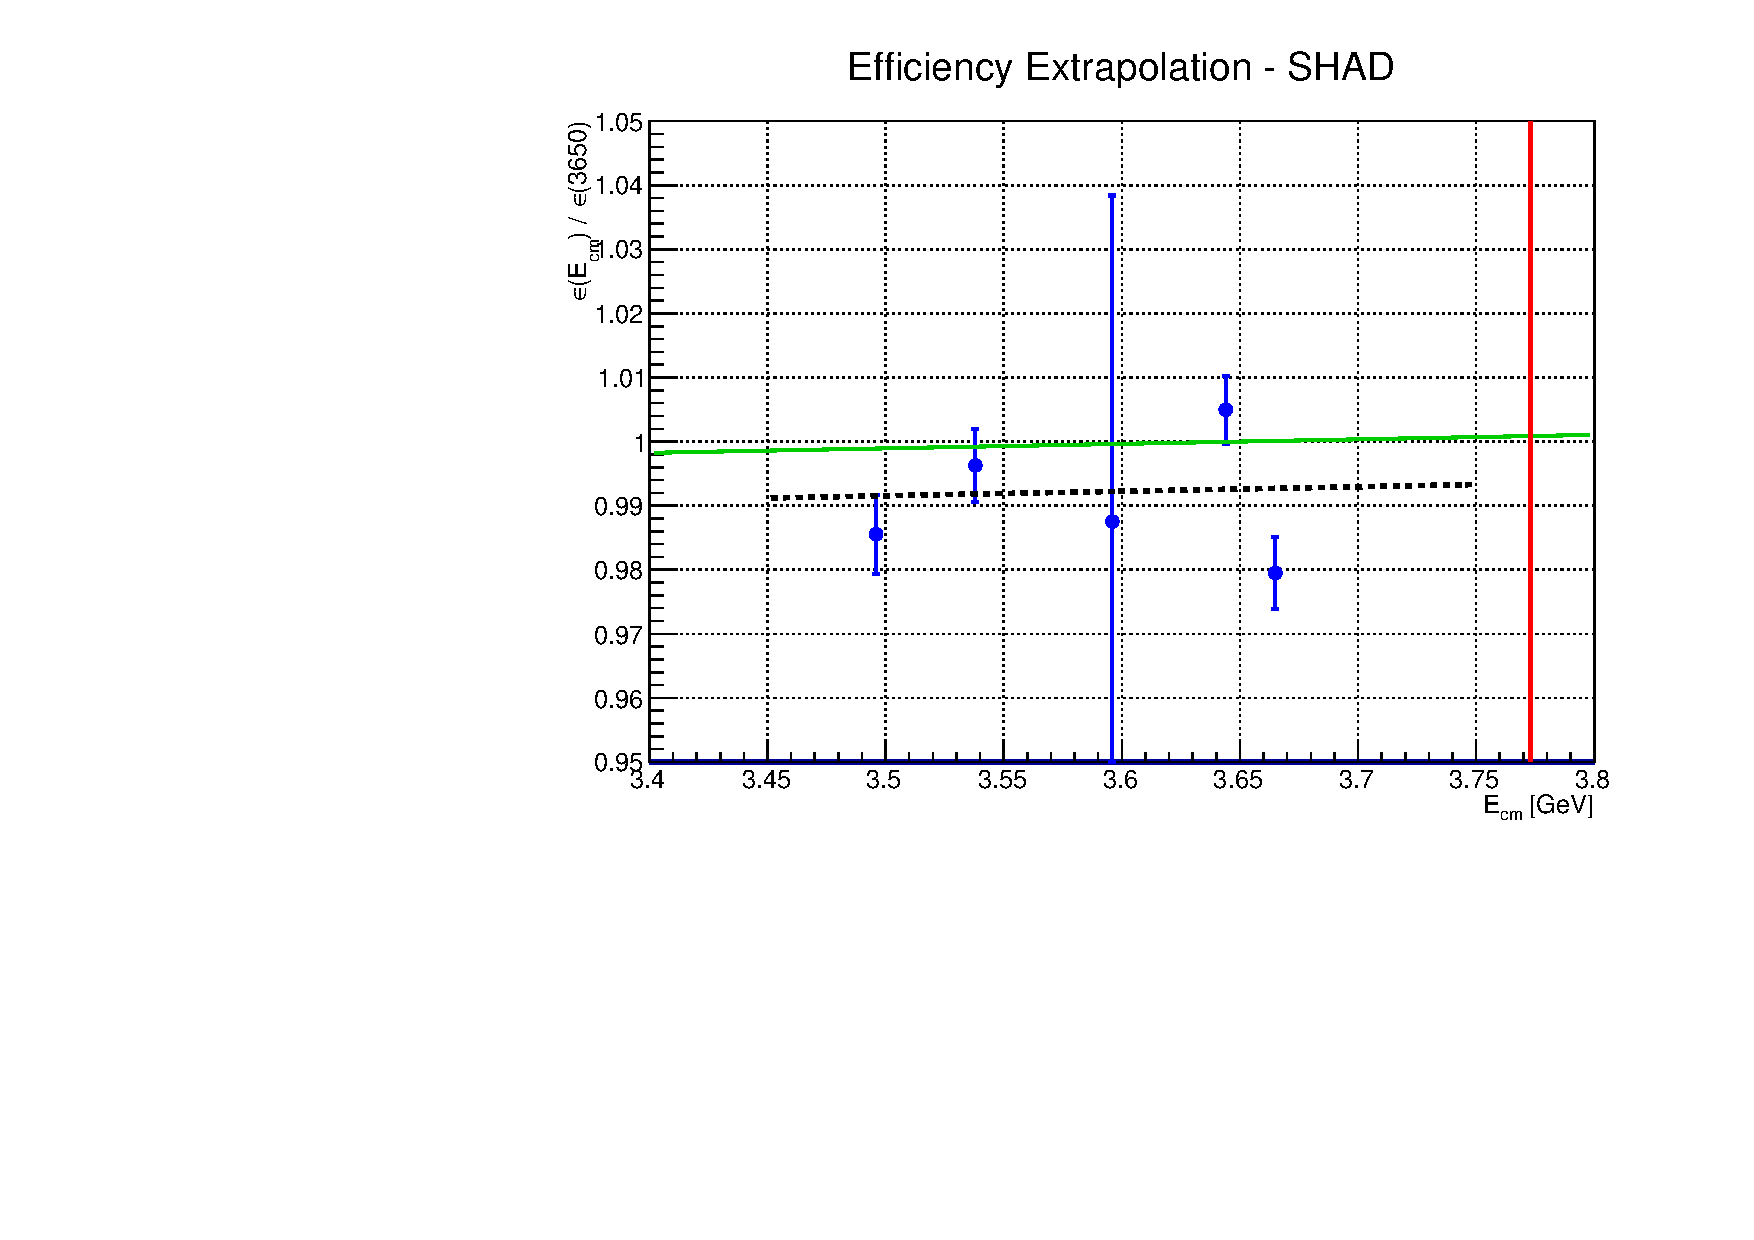
\includegraphics[scale=0.75]{figures/plots/SHAD_psip_BW.pdf}
\caption{The extrapolation for SHAD events using the new continuum data.}
{The new continuum points (blue) are fit using a linear slope (dashed black), then extrapolated to higher energies (solid green) based on the old continuum energy point at \SI{3.650}{\GeV} (cyan).
 The energy point for the $\psipp$ samples at \SI{3.773}{\GeV} is also shown (solid red).}
\label{fig:extrapolation_SHAD}
\end{figure}

\begin{figure}[H]
\centering
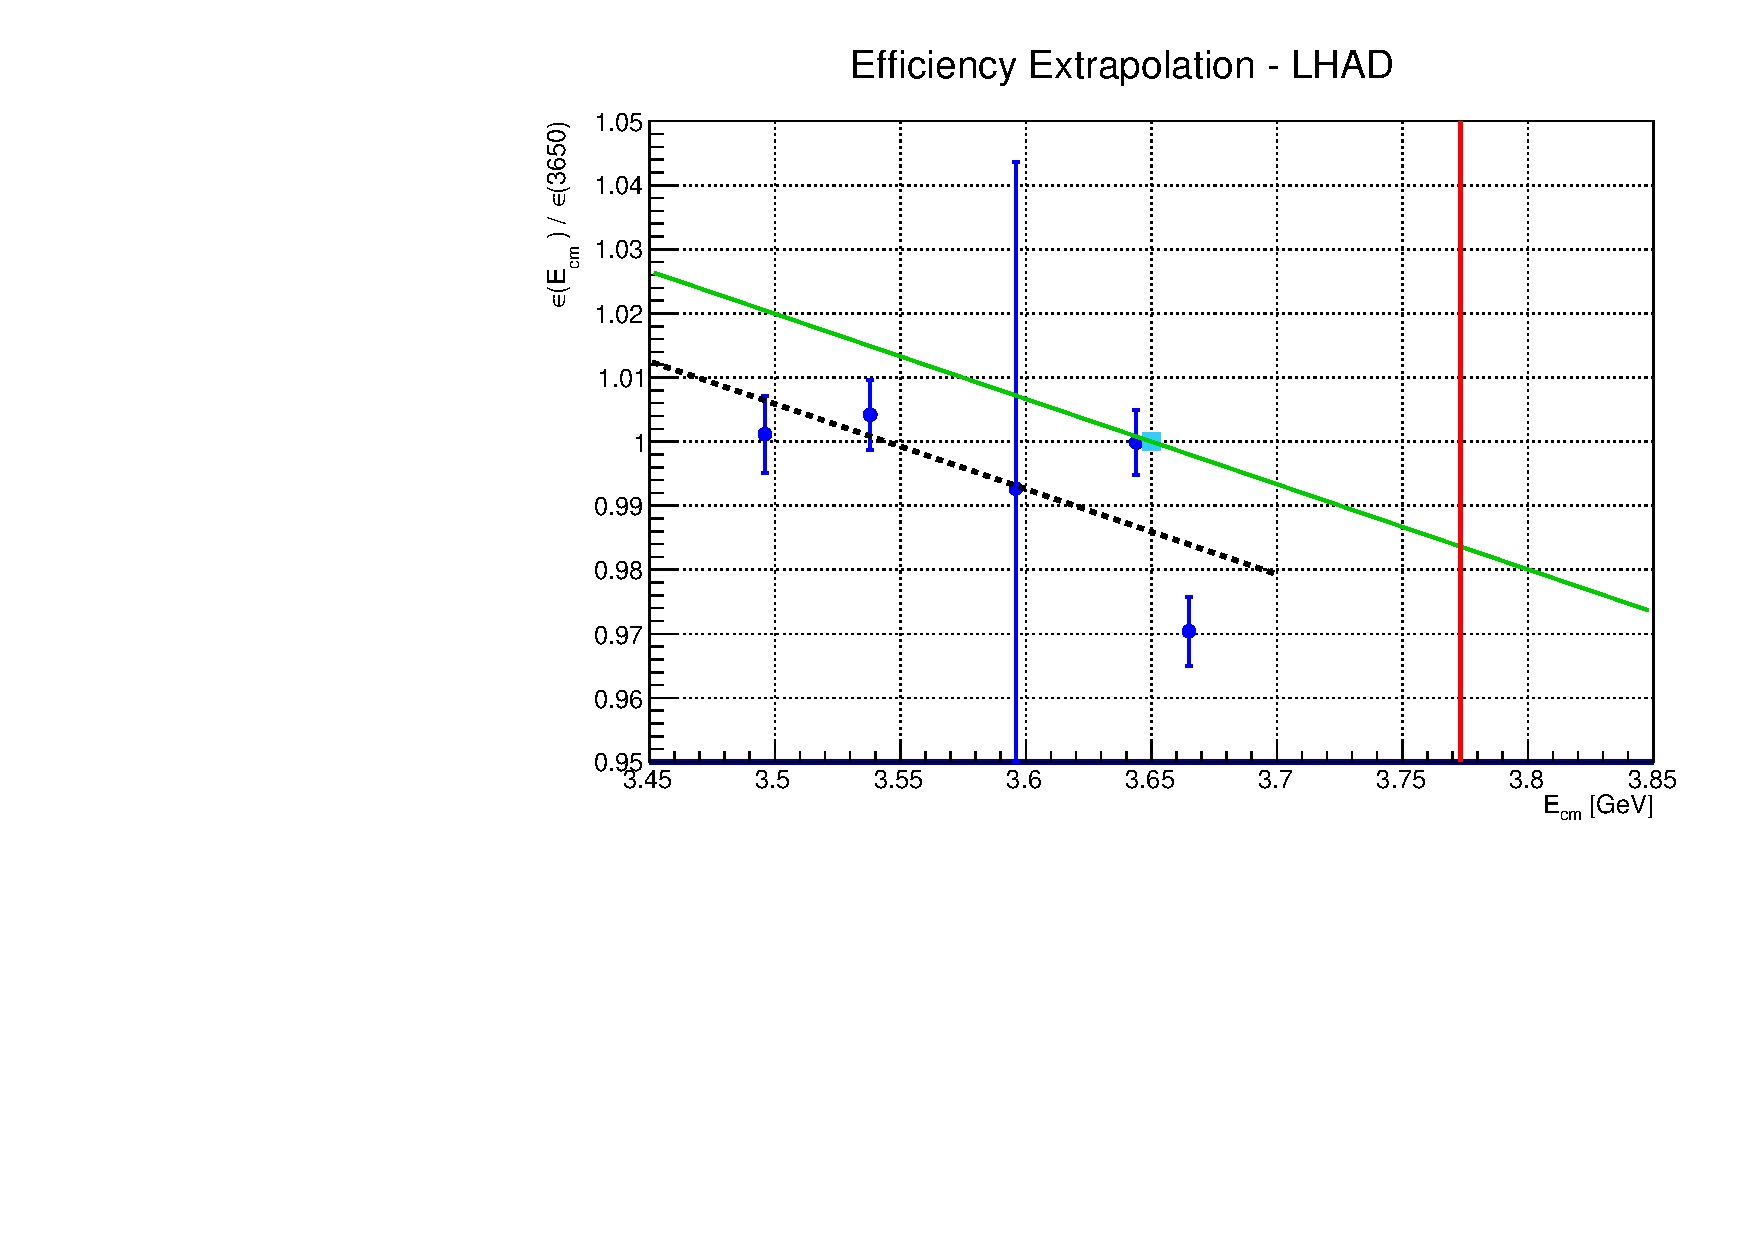
\includegraphics[scale=0.75]{figures/plots/LHAD_psip_BW.pdf}
\caption{The extrapolation for LHAD events using the new continuum data.}
{The new continuum points (blue) are fit using a linear slope (dashed black), then extrapolated to higher energies (solid green) based on the old continuum energy point at \SI{3.650}{\GeV} (cyan).
 The energy point for the $\psipp$ samples at \SI{3.773}{\GeV} is also shown (solid red).}
\label{fig:extrapolation_LHAD}
\end{figure}

\begin{figure}[H]
\centering
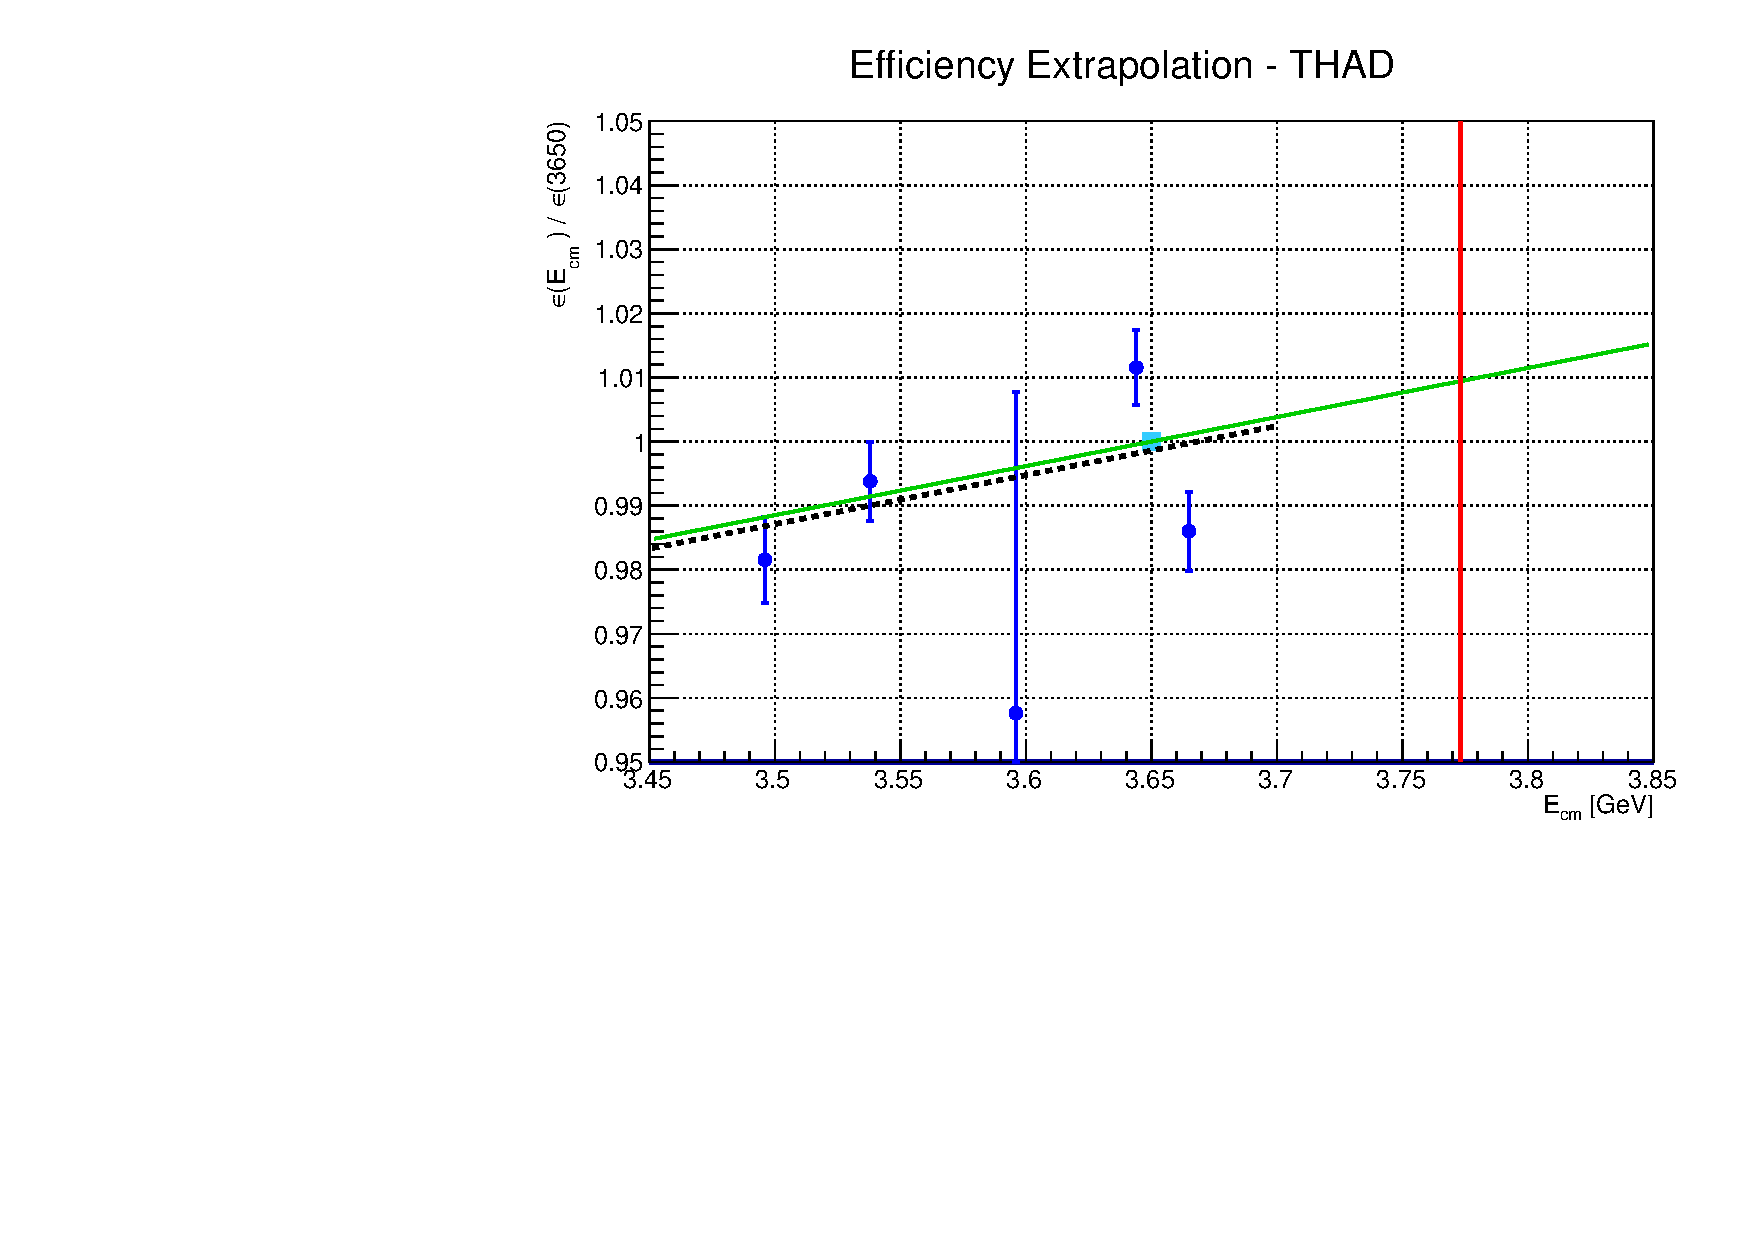
\includegraphics[scale=0.75]{figures/plots/THAD_psip_BW.pdf}
\caption{The extrapolation for THAD events using the new continuum data.}
{The new continuum points (blue) are fit using a linear slope (dashed black), then extrapolated to higher energies (solid green) based on the old continuum energy point at \SI{3.650}{\GeV} (cyan).
 The energy point for the $\psipp$ samples at \SI{3.773}{\GeV} is also shown (solid red).}
\label{fig:extrapolation_THAD}
\end{figure}

\pagebreak



\section{Results for $\psipp$ Data}
\label{sec:non_DDbar_results_psipp}

The procedure for determining the hadronic events in the $\psipp$ data is similar to the continuum region, but with certain modifications introduced due to the different relevant backgrounds.
Namely, above the $\DDbar$ peak, contributions from $\DO\aDO$ and $\Dp\Dm$ events must be accounted for.
Also, instead of the $\psip$ component, there is now a background from radiative $\psip$ production ($\ypsip$).
Lastly, due to the minimal contribution of two photon fusion events ($\twophoton$) in this region, this component is neglected for the $\psipp$ samples.
The counting of total hadronic events, however, functions identically to the continuum data, and the results are shown in \Cref{fig:hadron_fits_psipp_R1,fig:hadron_fits_psipp_R2}.

\begin{figure}[H]
\centering
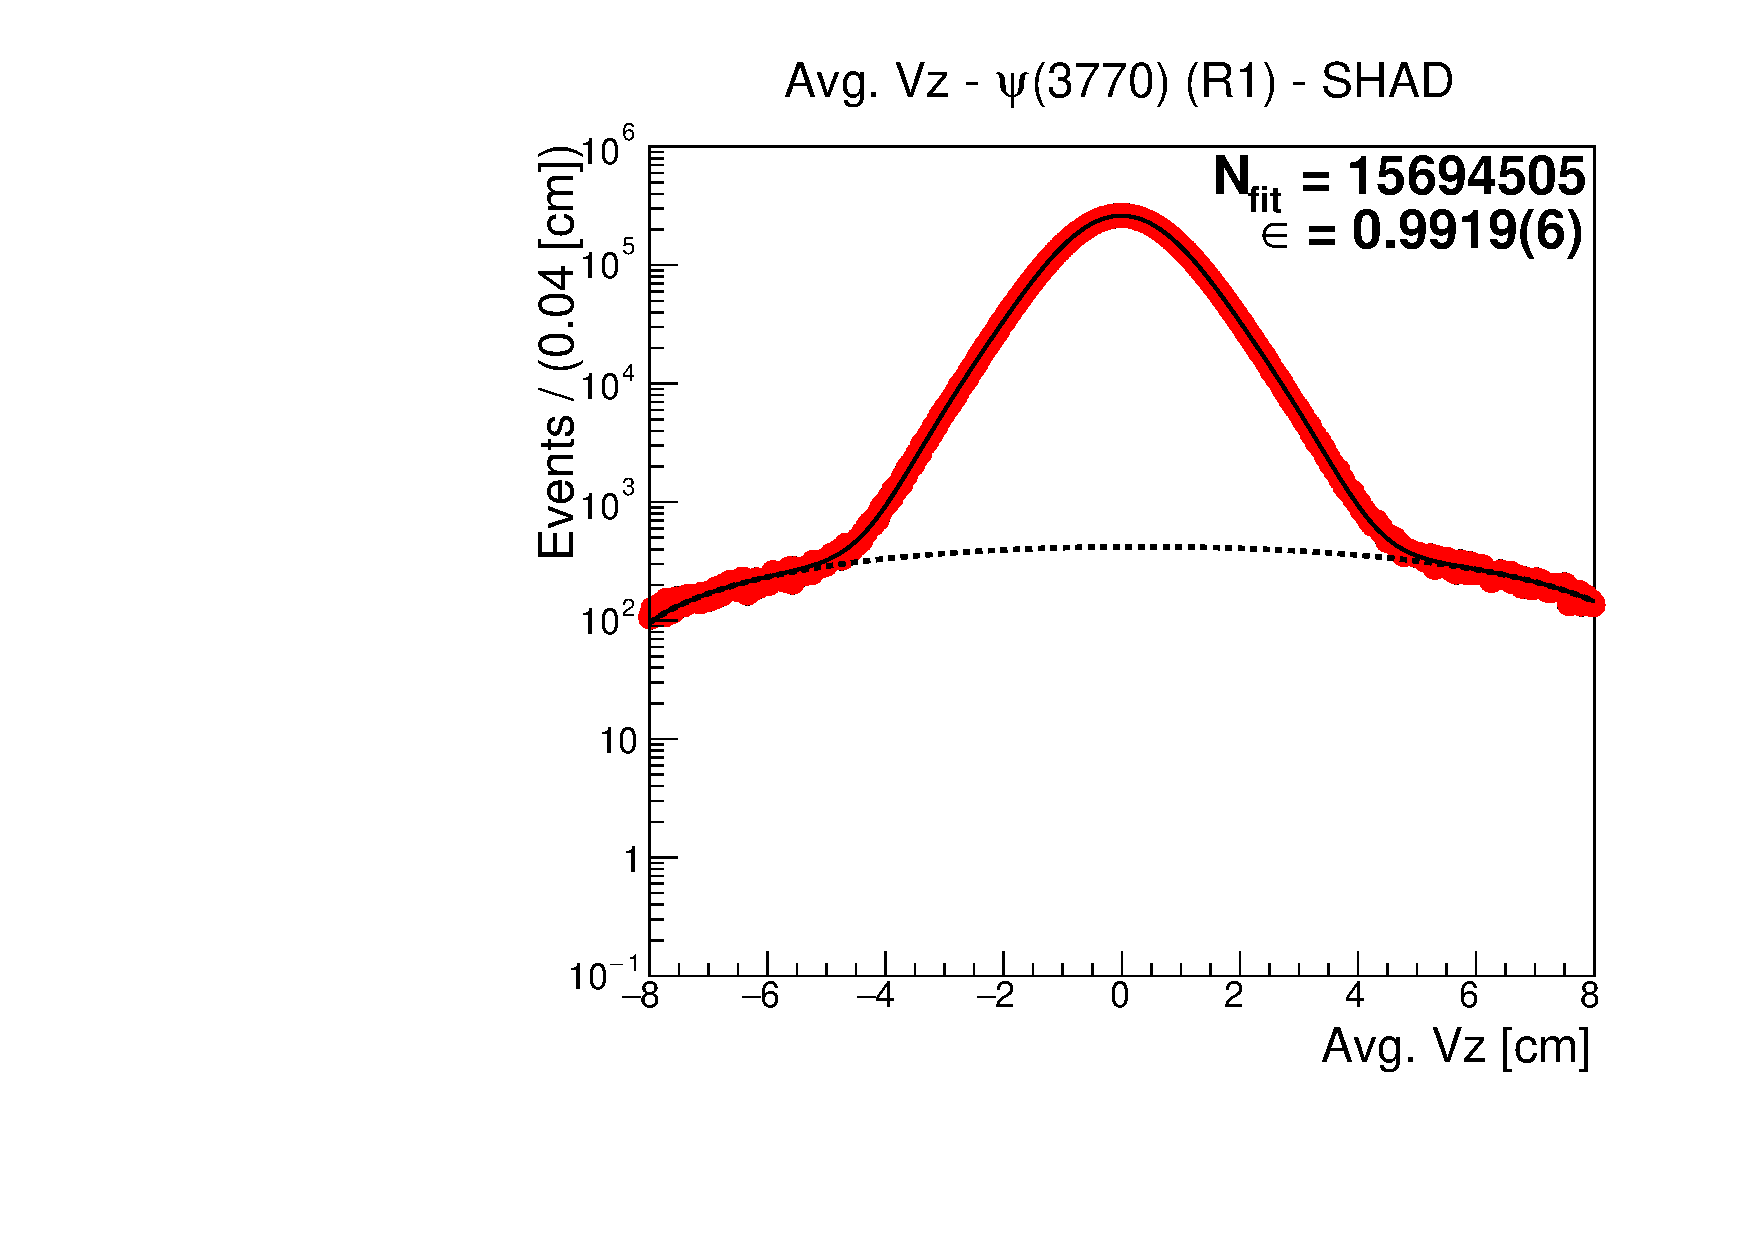
\includegraphics[scale=0.25]{figures/plots/nonDDbar_fit_results/psipp/fit_3773_R1_data_SHAD.pdf}
\hspace{-0.5cm}
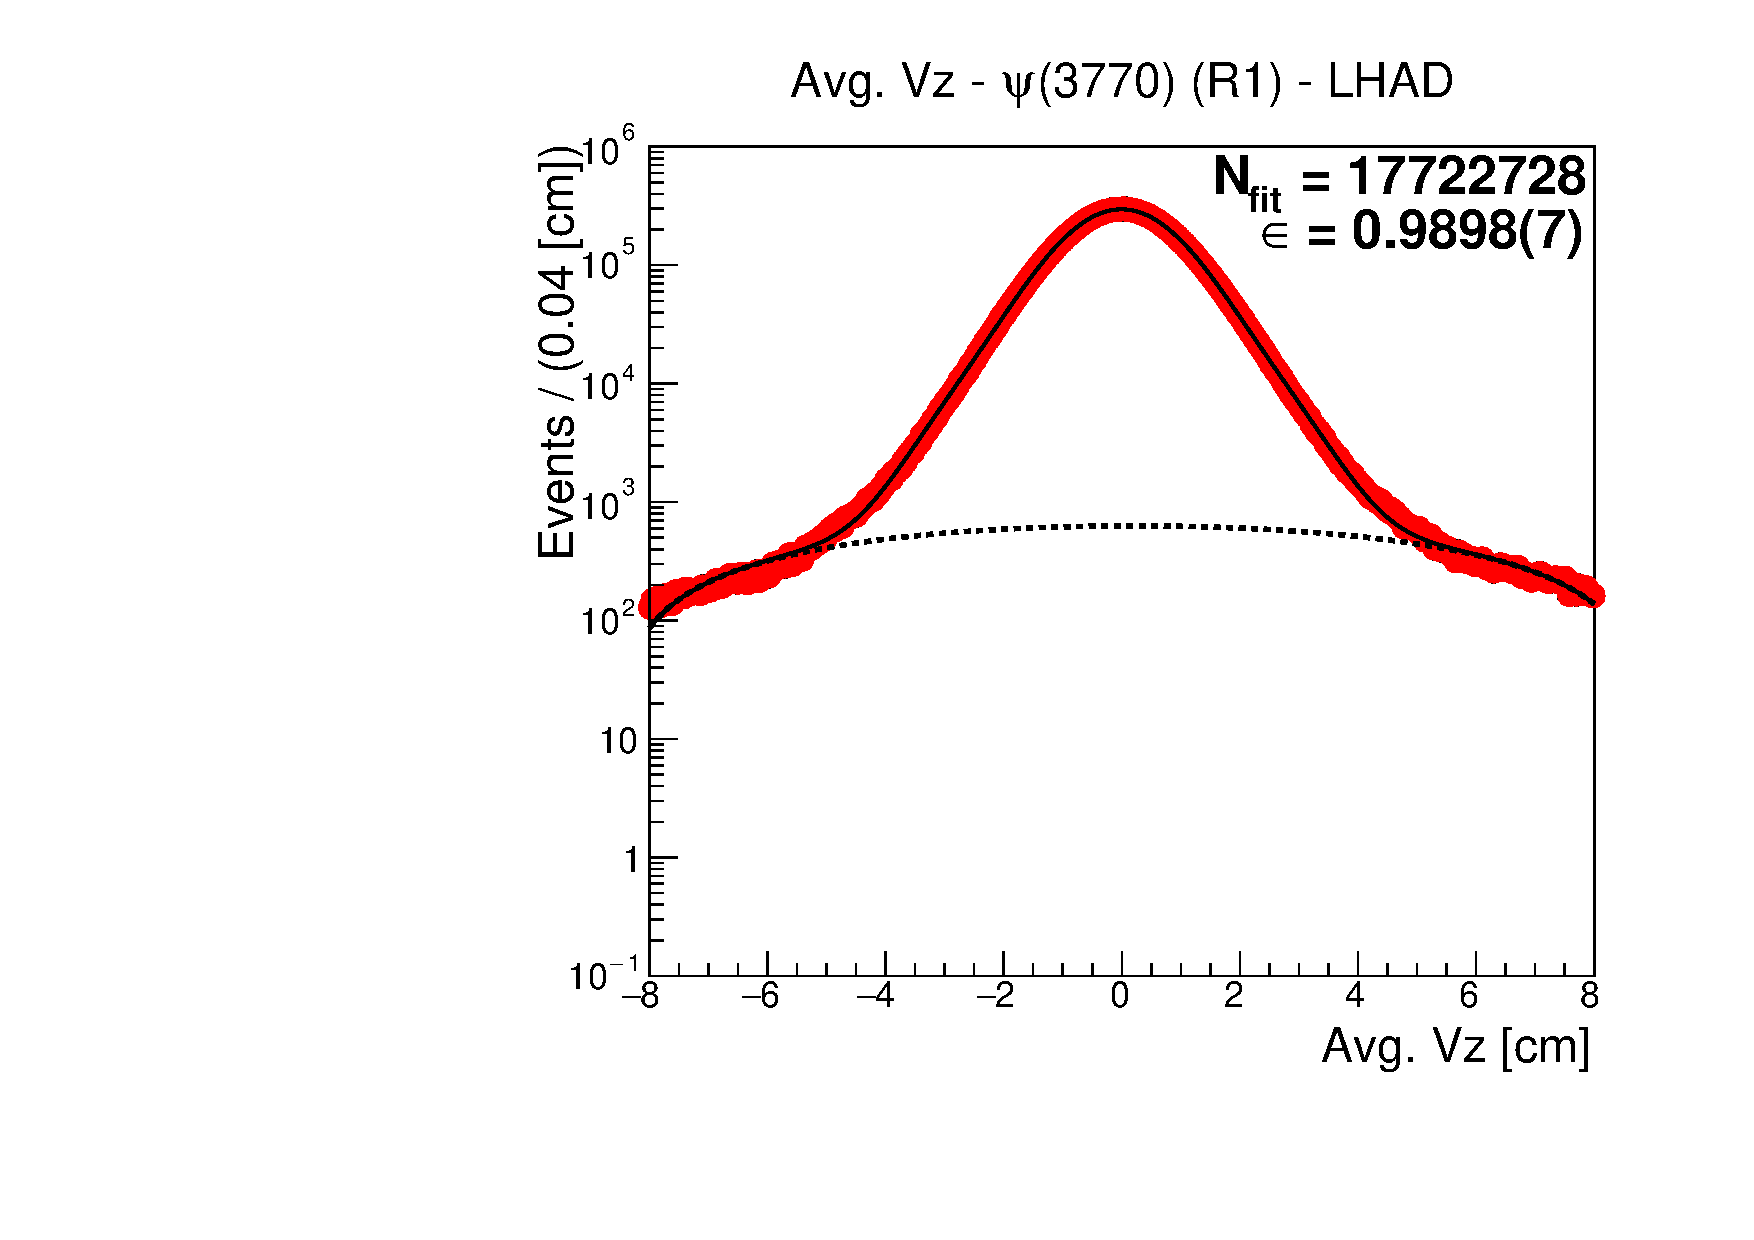
\includegraphics[scale=0.25]{figures/plots/nonDDbar_fit_results/psipp/fit_3773_R1_data_LHAD.pdf}
\hspace{-0.5cm}
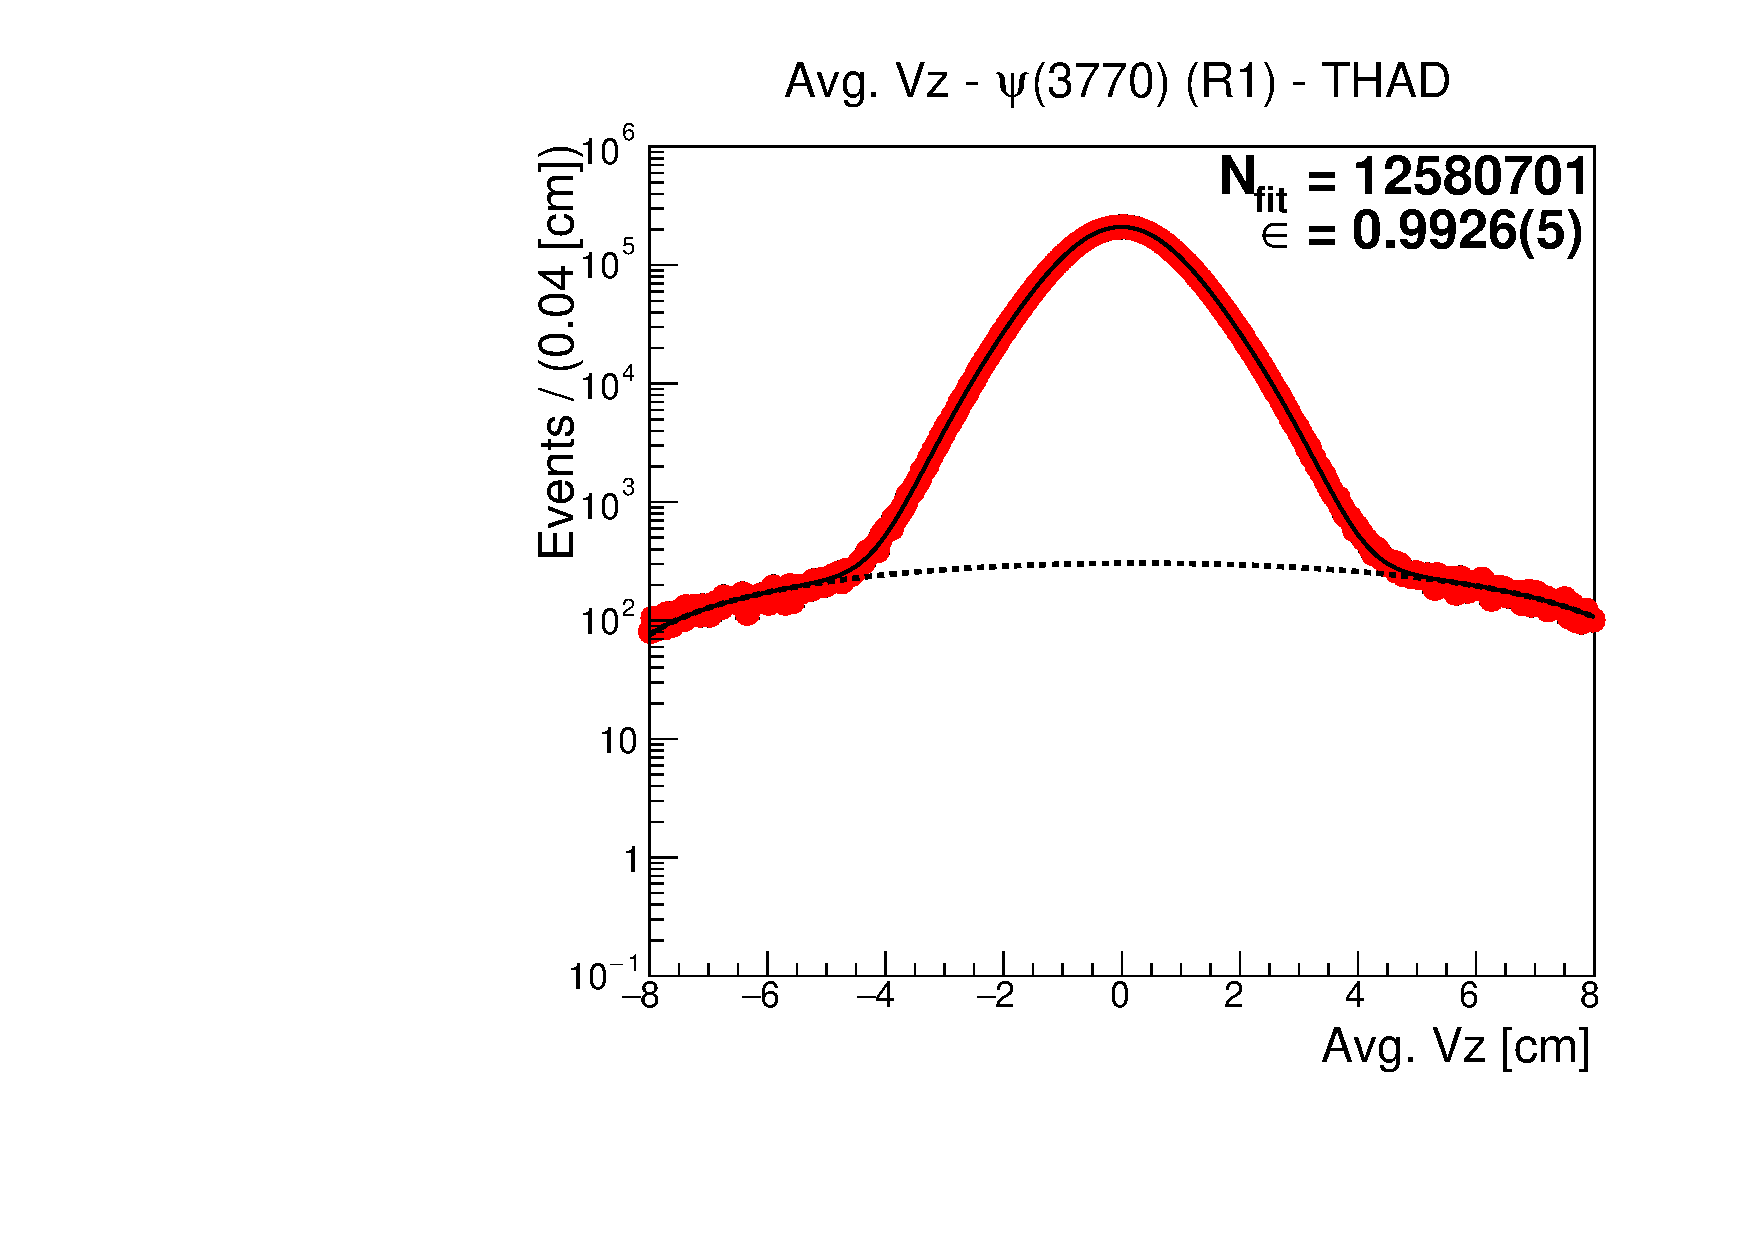
\includegraphics[scale=0.25]{figures/plots/nonDDbar_fit_results/psipp/fit_3773_R1_data_THAD.pdf}
\caption{The number of hadrons found in the $\psipp$ (R1) data sample.}
{This includes results for SHAD (left), LHAD (middle), and THAD (right).}
\label{fig:hadron_fits_psipp_R1}
\end{figure}


\begin{figure}[H]
\centering
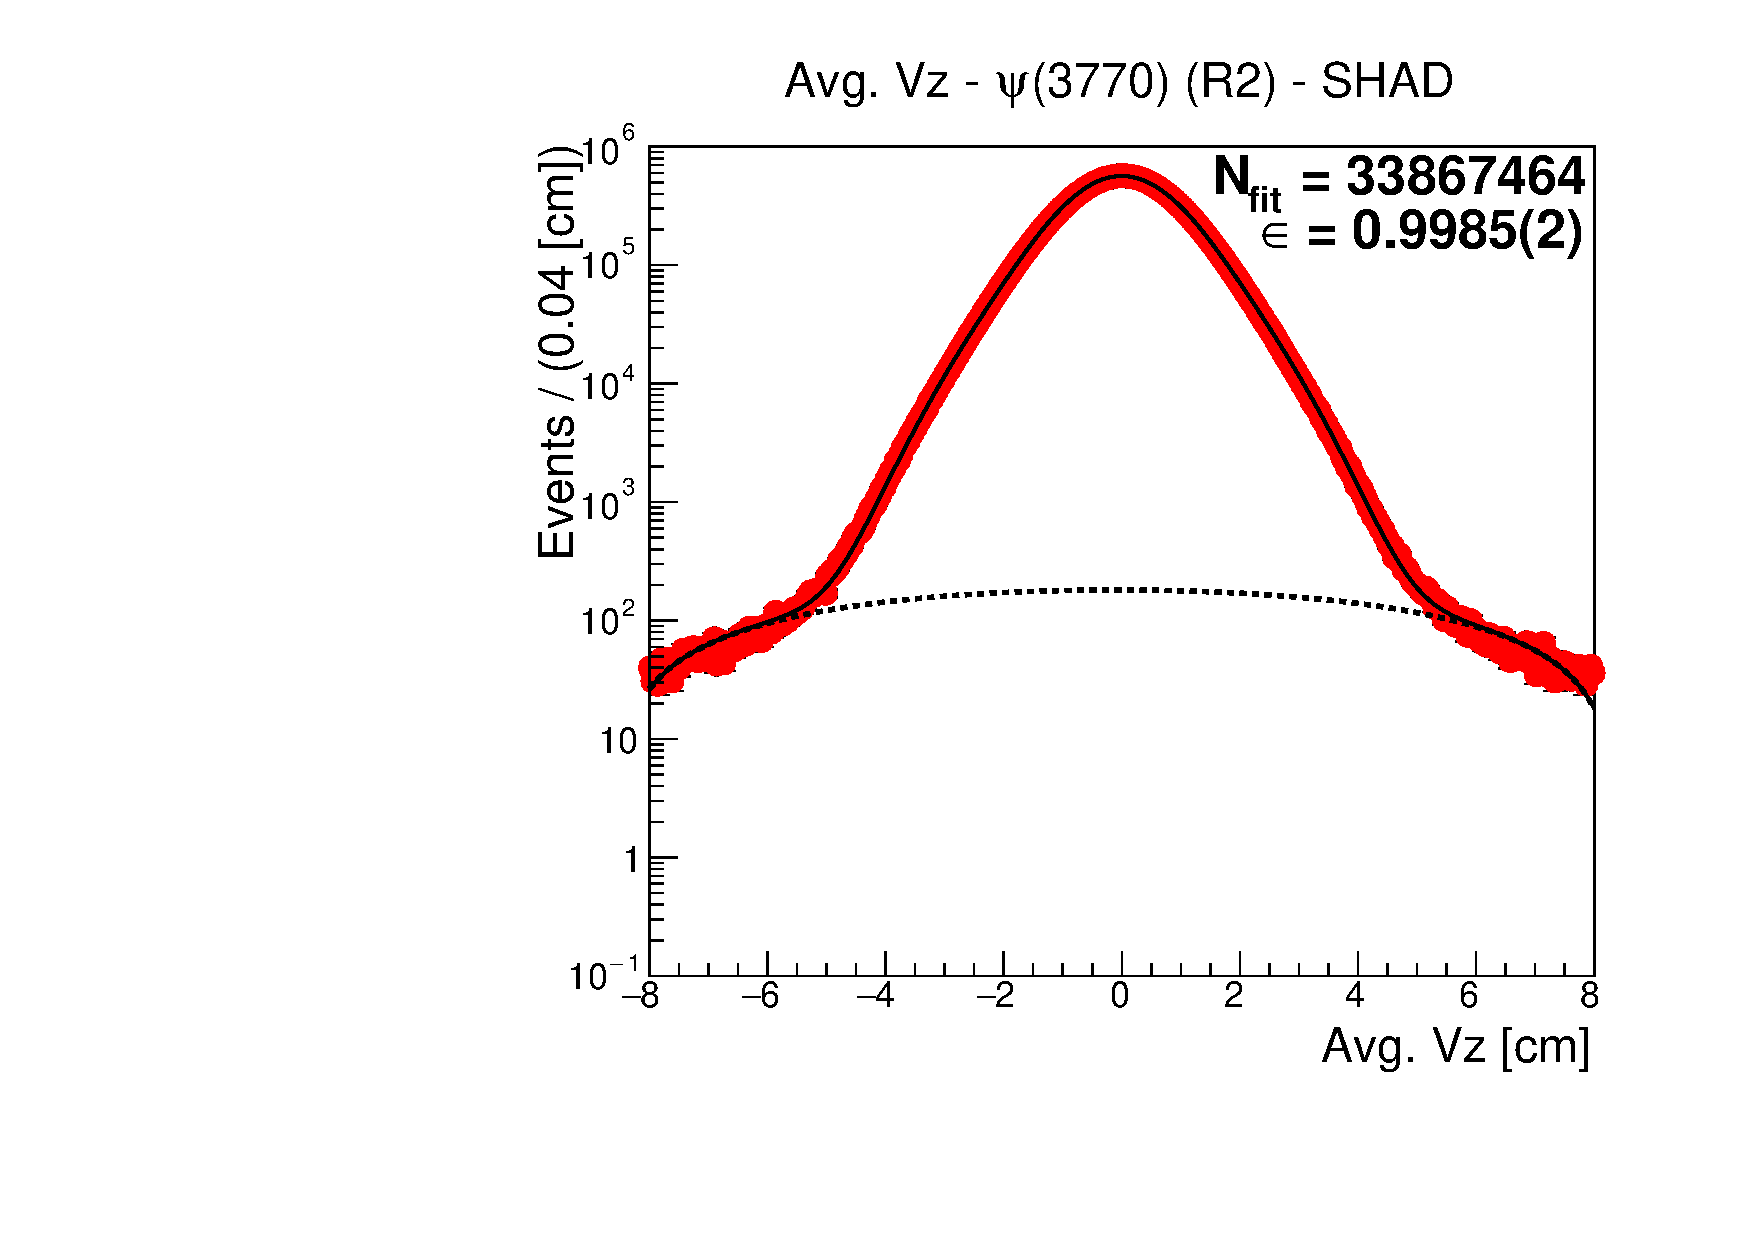
\includegraphics[scale=0.25]{figures/plots/nonDDbar_fit_results/psipp/fit_3773_R2_data_SHAD.pdf}
\hspace{-0.5cm}
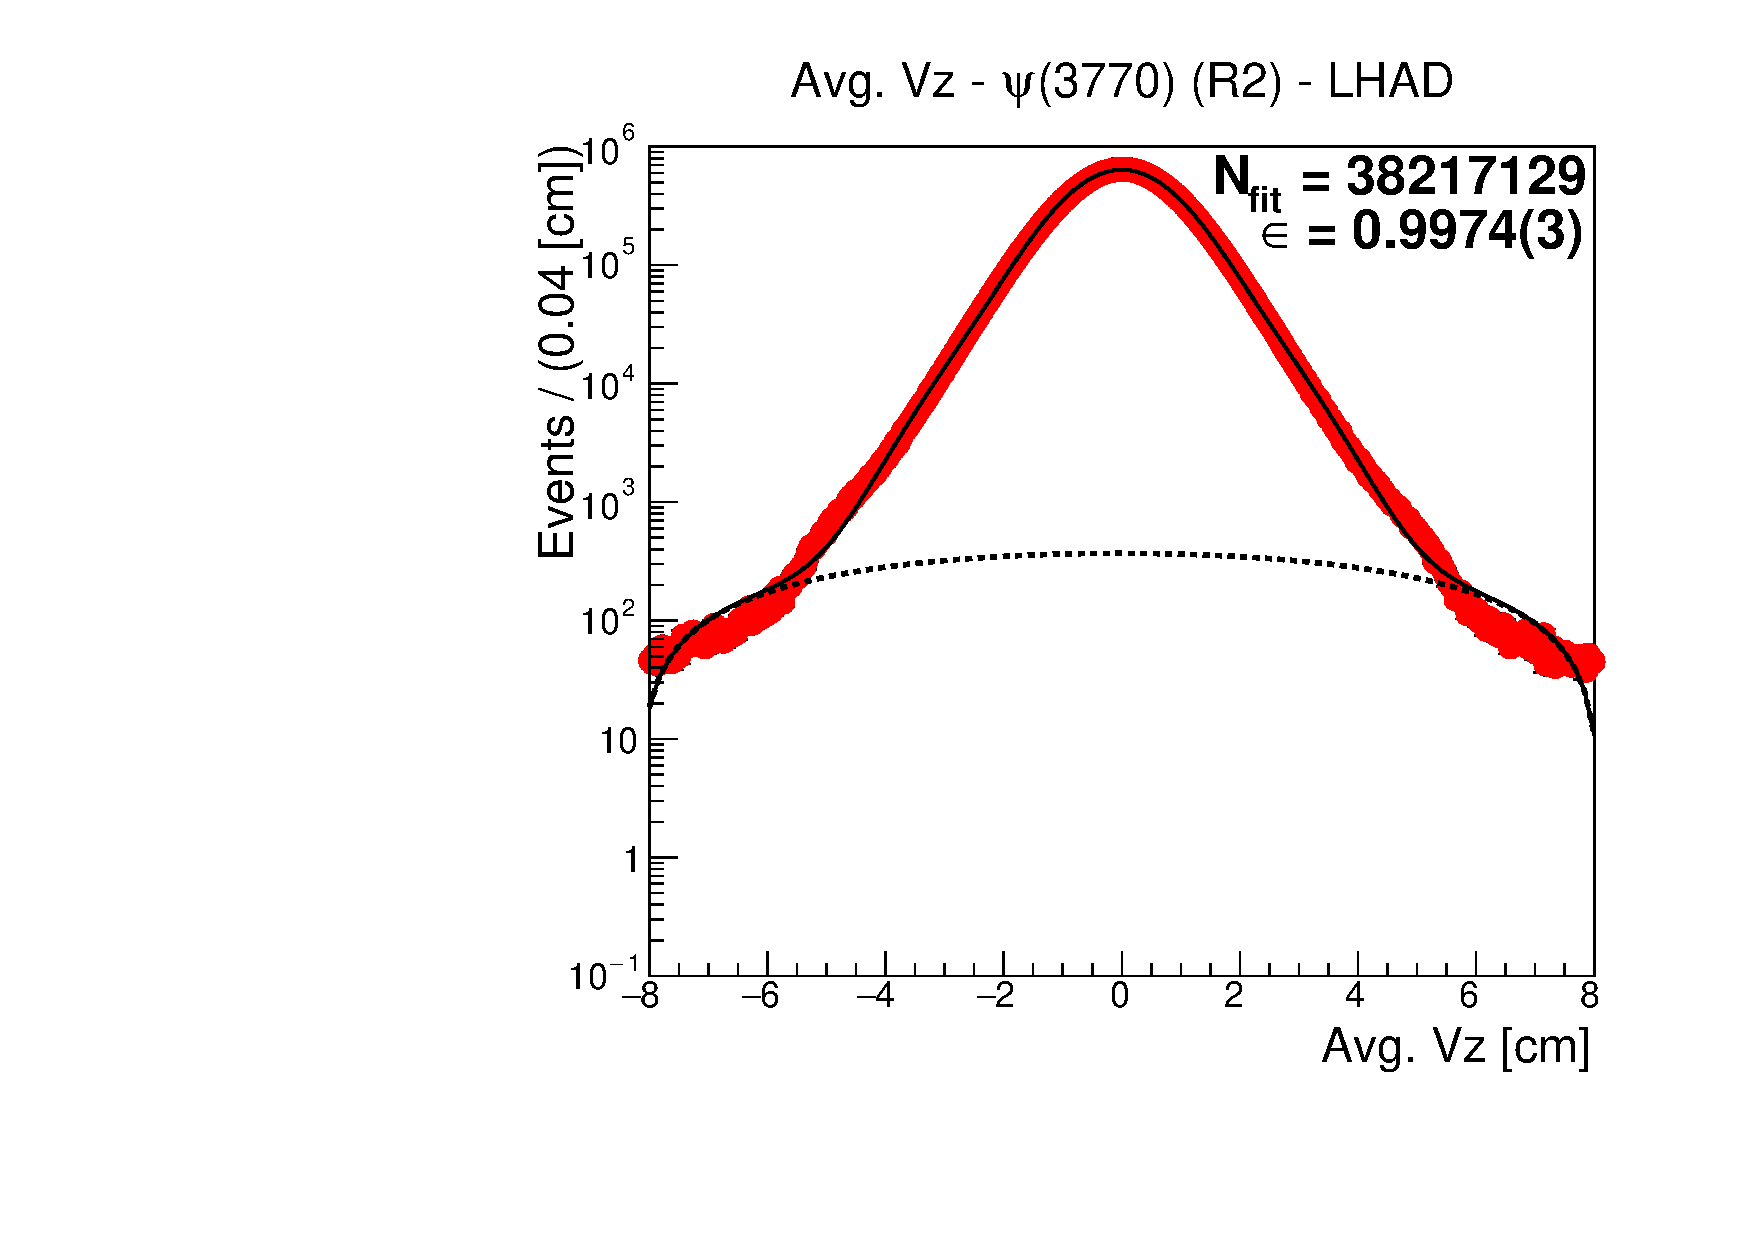
\includegraphics[scale=0.25]{figures/plots/nonDDbar_fit_results/psipp/fit_3773_R2_data_LHAD.pdf}
\hspace{-0.5cm}
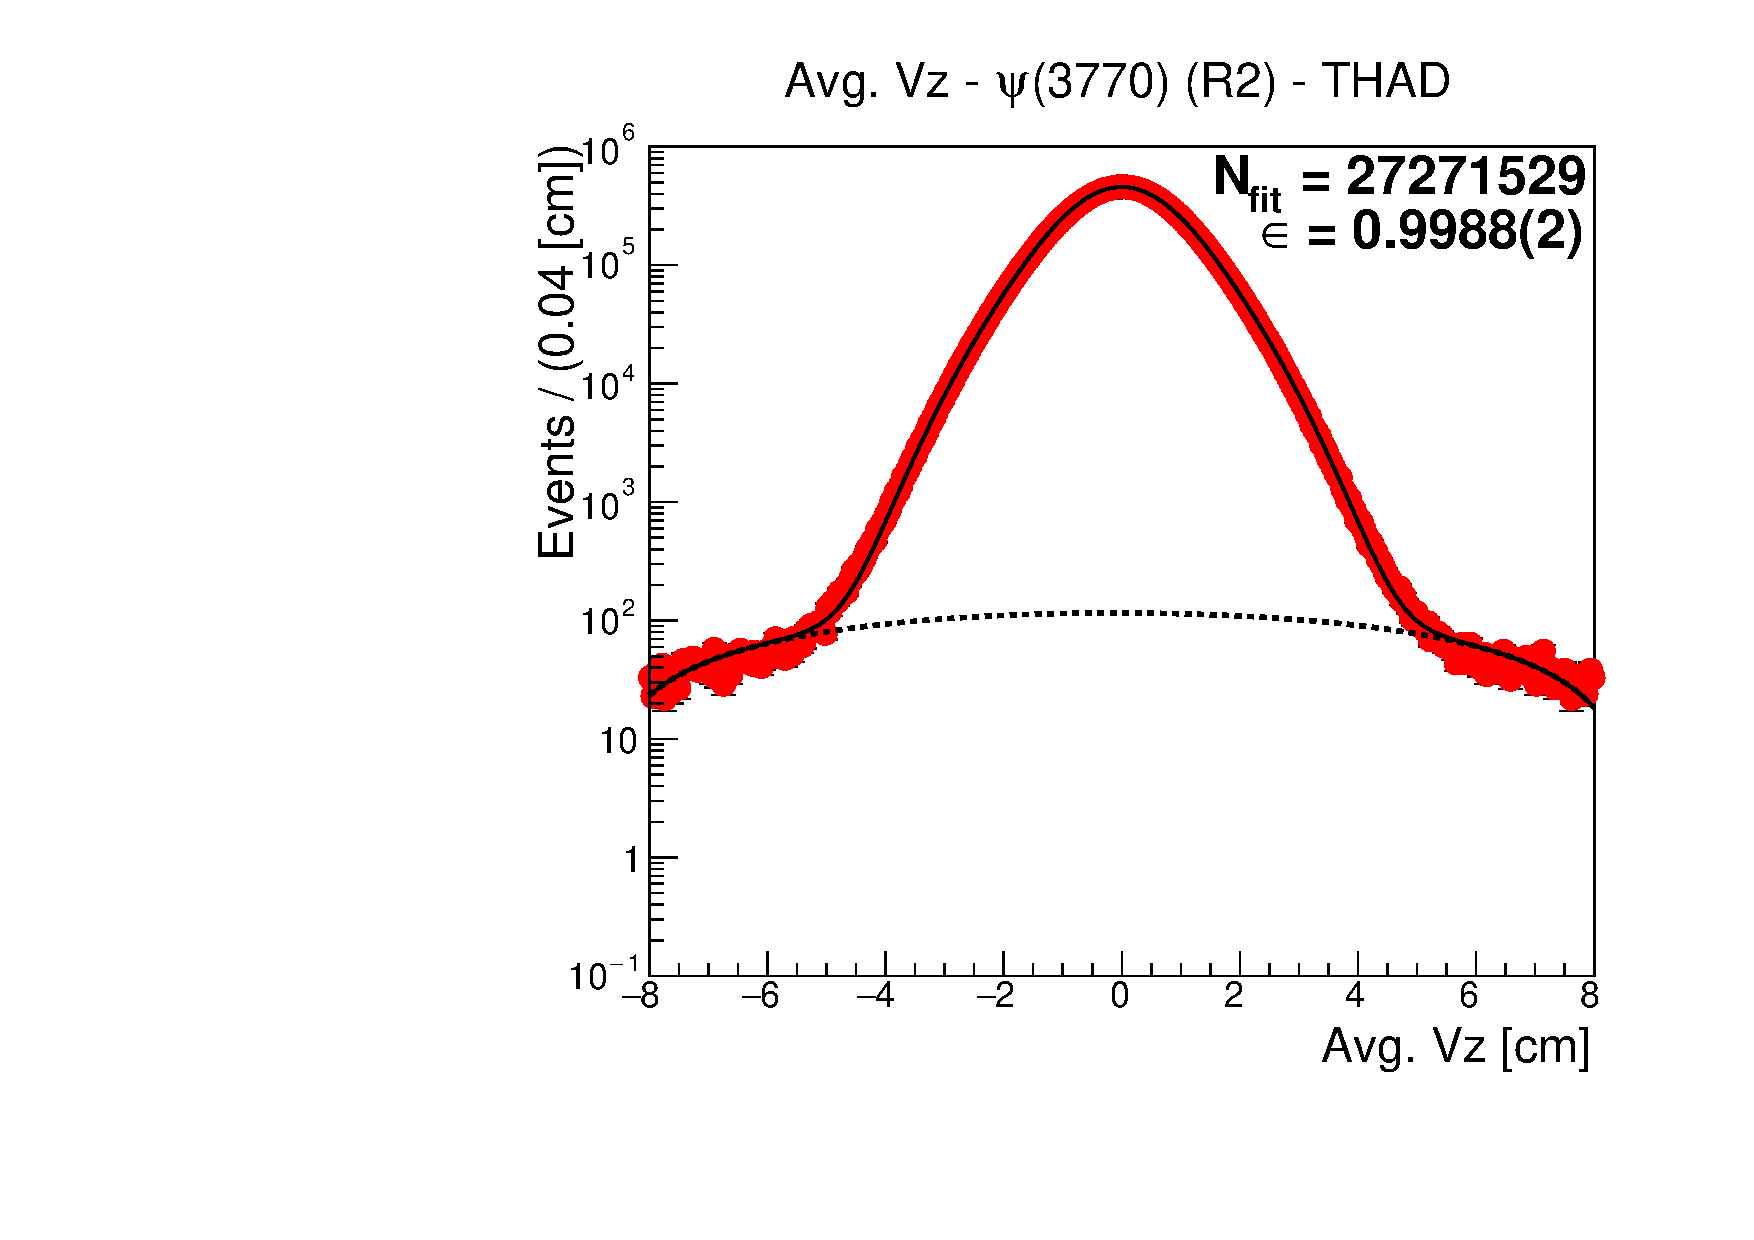
\includegraphics[scale=0.25]{figures/plots/nonDDbar_fit_results/psipp/fit_3773_R2_data_THAD.pdf}
\caption{The number of hadrons found in the $\psipp$ (R2) data sample.}
{This includes results for SHAD (left), LHAD (middle), and THAD (right).}
\label{fig:hadron_fits_psipp_R2}
\end{figure}


\subsection{$\DDbar$ Correction}
\label{ssec:DDbar_correction}

Since the $\DDbar$ cross section is not a smooth scaling of energy (like $\qqbar$), we must precisely determine its reconstruction efficiency using data.
Instead of using the standard definition of $\effmc$ for $\DDbar$, we apply a correction based on the multiplicity of $\DDbar$ events in both data and MC.
This is done by finding single-tagged $D$ candidates and counting the number of tracks not used for reconstruction.
By randomly sampling pairs of points from this distribution, and assuming the decays are uncorrelated, we can produce an average representation of multiplicity in $\DDbar$ events.
From this new distribution, selections methods for SHAD, LHAD, and THAD are performed based off number of tracks selected by the simplified cut criteria shown in \Cref{tab:DDbar_corr_cuts} relative to the total.
The corrections applied to each efficiency are the ratio of these selections in data and MC.
As the $\psipp$ samples for R1 and R2 were taken at different times, they are treated separately for this process.
The results for each are shown in \Cref{tab:DDbar_corr_results} with the corresponding distributions shown in \Cref{fig:DD_corr_D0_R1,fig:DD_corr_Dp_R1,fig:DD_corr_D0_R2,fig:DD_corr_Dp_R2}.
 
\begin{table}[H]
\centering
\renewcommand\arraystretch{1.0}
\begin{tabular}{c|c}
\hline
Selection Method & Number of Tracks \\
\hline
SHAD & $\Ntrk > 2$ \\
LHAD & $\Ntrk > 1$ \\
THAD & $\Ntrk > 3$ \\
\hline
\end{tabular}
\caption{Selection methods for the $\DDbar$ efficiency correction.}
\label{tab:DDbar_corr_cuts}
\end{table}
 
\begin{table}[H]
\centering
\renewcommand\arraystretch{1.0}
\begin{tabular}{c|c c|c c}
\hline
                 & \multicolumn{2}{c|}{$\psipp$ R1} & \multicolumn{2}{c}{$\psipp$ R2} \\
\hline
Selection & $(\effdata / \effmc) \; (\DO)$ & $(\effdata / \effmc) \; (\Dp)$ & $(\effdata / \effmc) \; (\DO)$ & $(\effdata / \effmc) \; (\Dp)$ \\
\hline
SHAD & 0.9751 & 0.9992 & 0.9759 & 0.9999 \\
LHAD & 0.9930 & 1.0018 & 0.9935 & 1.0024 \\
THAD & 0.9662 & 1.0064 & 0.9684 & 1.0108 \\
\hline
\end{tabular}
\caption{Efficiency corrections for the $\psipp$ samples.}
{The corrections are impactful for $\DO$, but minimal for $\Dp$.
This is due to the differences in their low-side other $D$ multiplicities, as seen in \Cref{fig:DD_corr_D0_R1,fig:DD_corr_Dp_R1,fig:DD_corr_D0_R2,fig:DD_corr_Dp_R2}.}
\label{tab:DDbar_corr_results}
\end{table}


\begin{figure}[H]
\centering
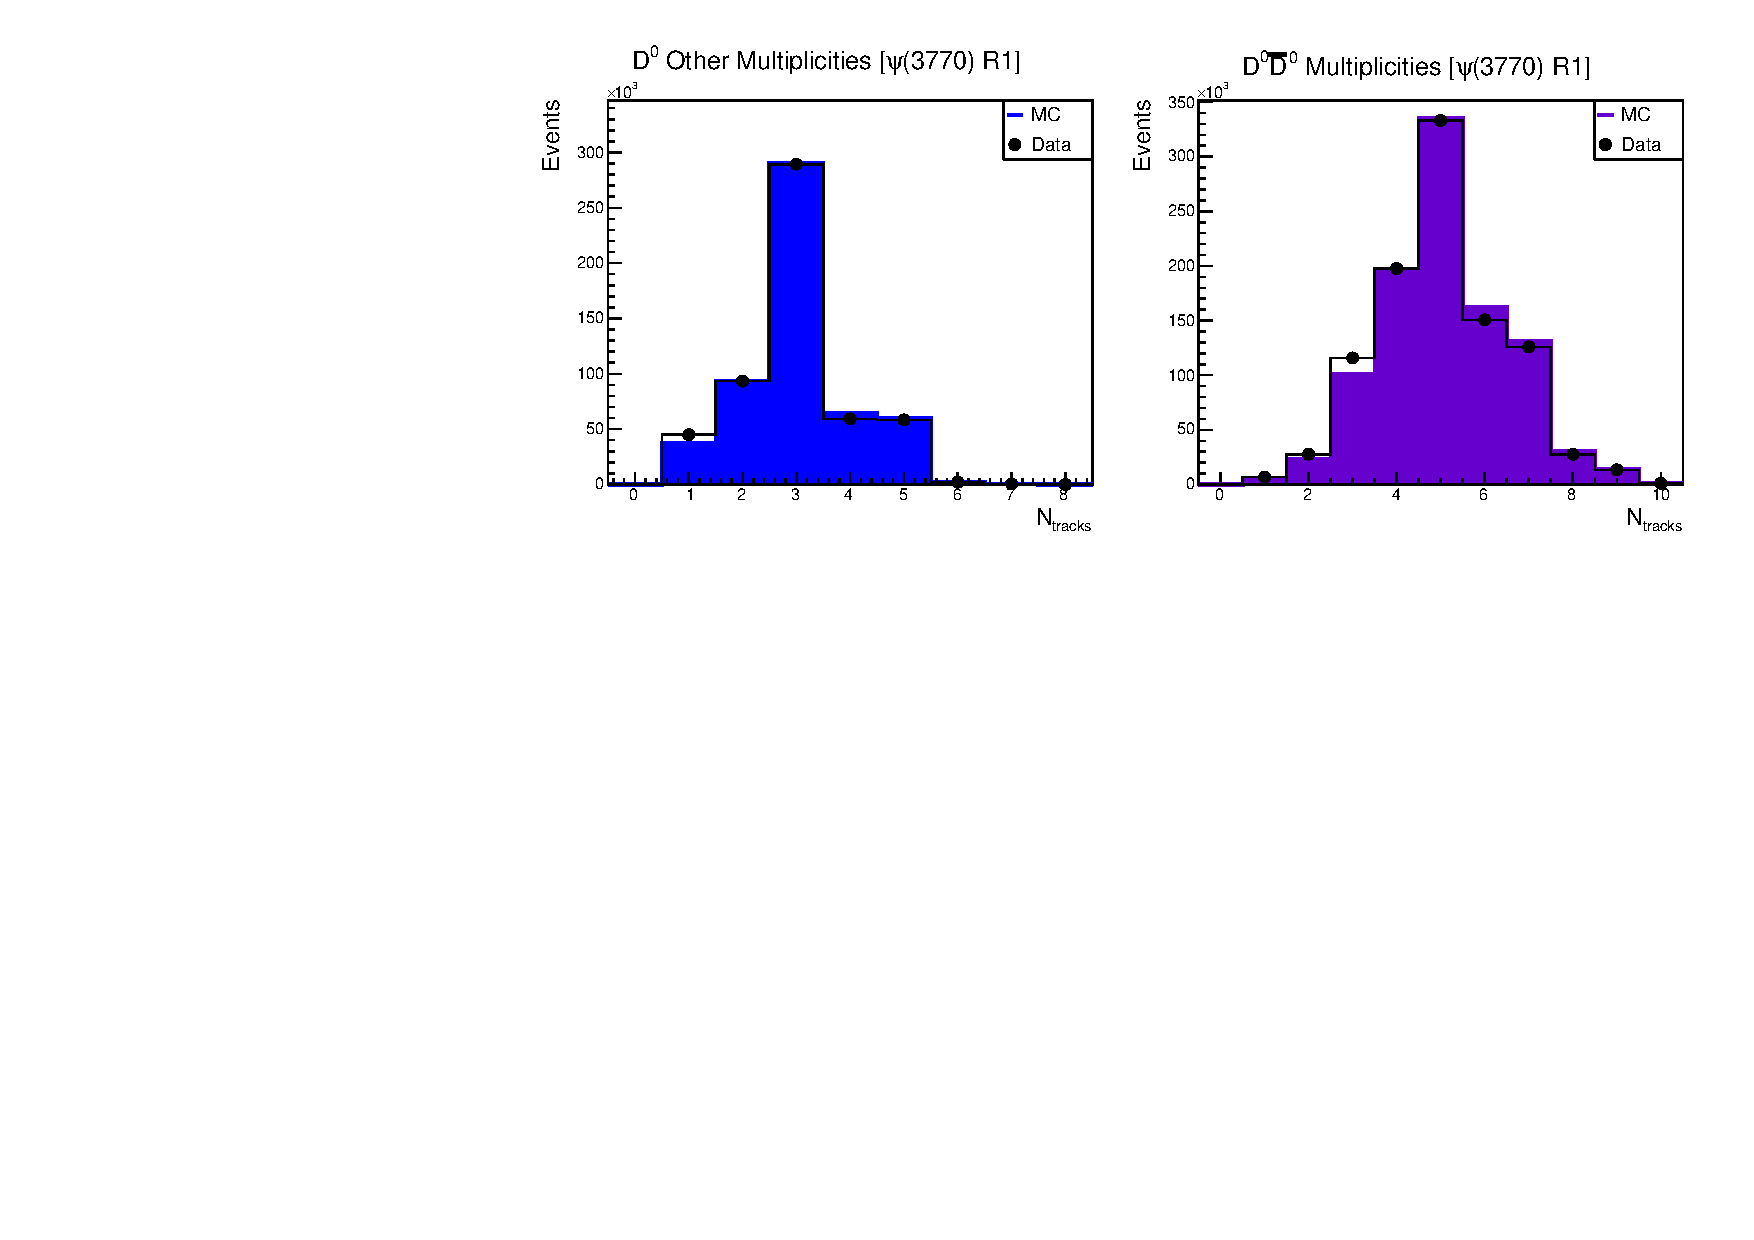
\includegraphics[scale=0.75]{figures/plots/DD_corr_plots/DD_psipp_D0D0bar_R1.pdf}
\caption{The other-side $\DO$ tracks and corresponding $\DO\aDO$ multiplicities for R1.}
{The distribution of good tracks not used for reconstruction of single-tagged $\DO$ particles (left) is randomly sampled for pairs of points which comprise the total multiplicity distribution (right).
The tracks in the $\DO\aDO$ multiplicity distribution are used to determine the efficiency correction based off the cuts in \Cref{tab:DDbar_corr_cuts}.}
\label{fig:DD_corr_D0_R1}
\end{figure}


\begin{figure}[H]
\centering
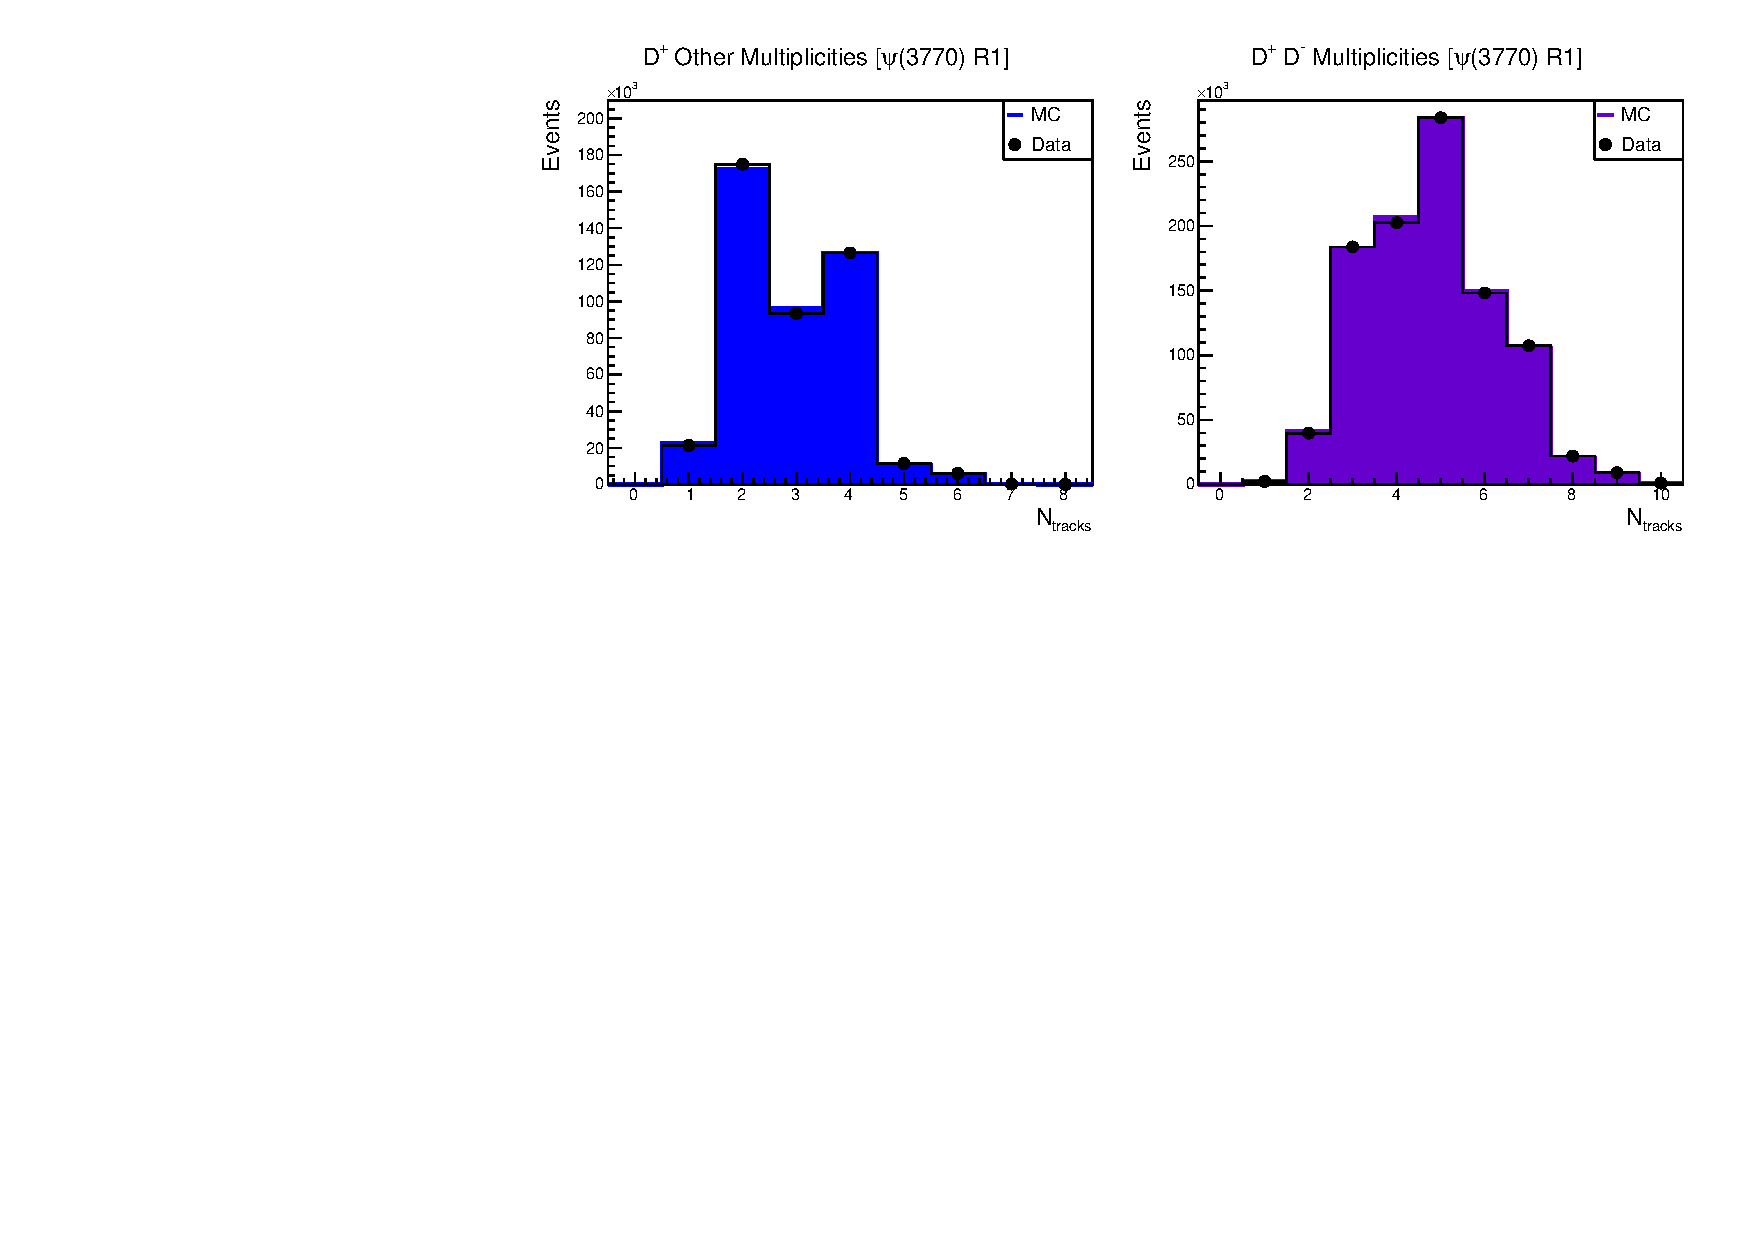
\includegraphics[scale=0.75]{figures/plots/DD_corr_plots/DD_psipp_DpDm_R1.pdf}
\caption{The other-side $\Dp$ tracks and corresponding $\Dp\Dm$ multiplicities for R1.}
{The distribution of good tracks not used for reconstruction of single-tagged $\Dp$ particles (left) is randomly sampled for pairs of points which comprise the total multiplicity distribution (right).
The tracks in the $\Dp\Dm$ multiplicity distribution are used to determine the efficiency correction based off the cuts in \Cref{tab:DDbar_corr_cuts}.}
\label{fig:DD_corr_Dp_R1}
\end{figure}


\begin{figure}[H]
\centering
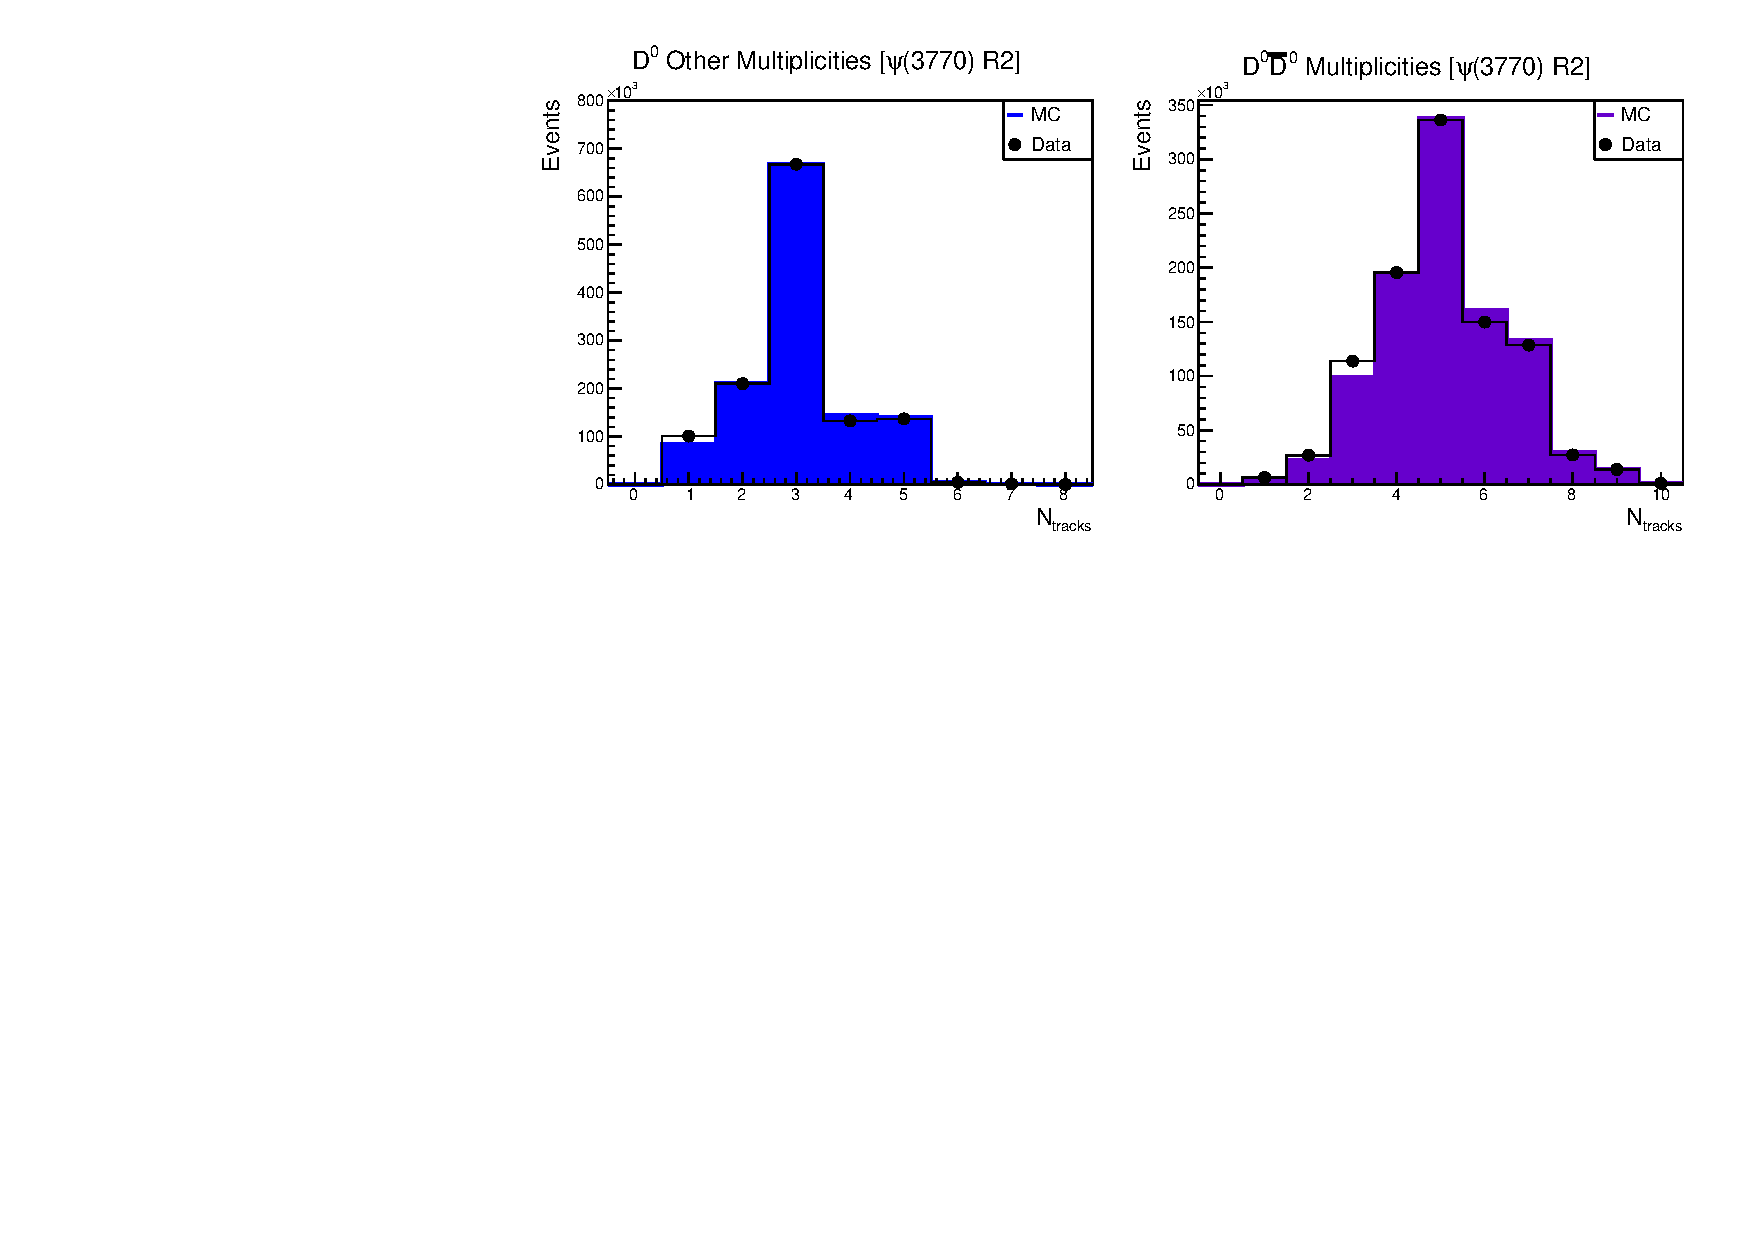
\includegraphics[scale=0.75]{figures/plots/DD_corr_plots/DD_psipp_D0D0bar_R2.pdf}
\caption{The other-side $\DO$ tracks and corresponding $\DO\aDO$ multiplicities for R2.}
{The distribution of good tracks not used for reconstruction of single-tagged $\DO$ particles (left) is randomly sampled for pairs of points which comprise the total multiplicity distribution (right).
The tracks in the $\DO\aDO$ multiplicity distribution are used to determine the efficiency correction based off the cuts in \Cref{tab:DDbar_corr_cuts}.}
\label{fig:DD_corr_D0_R2}
\end{figure}


\begin{figure}[H]
\centering
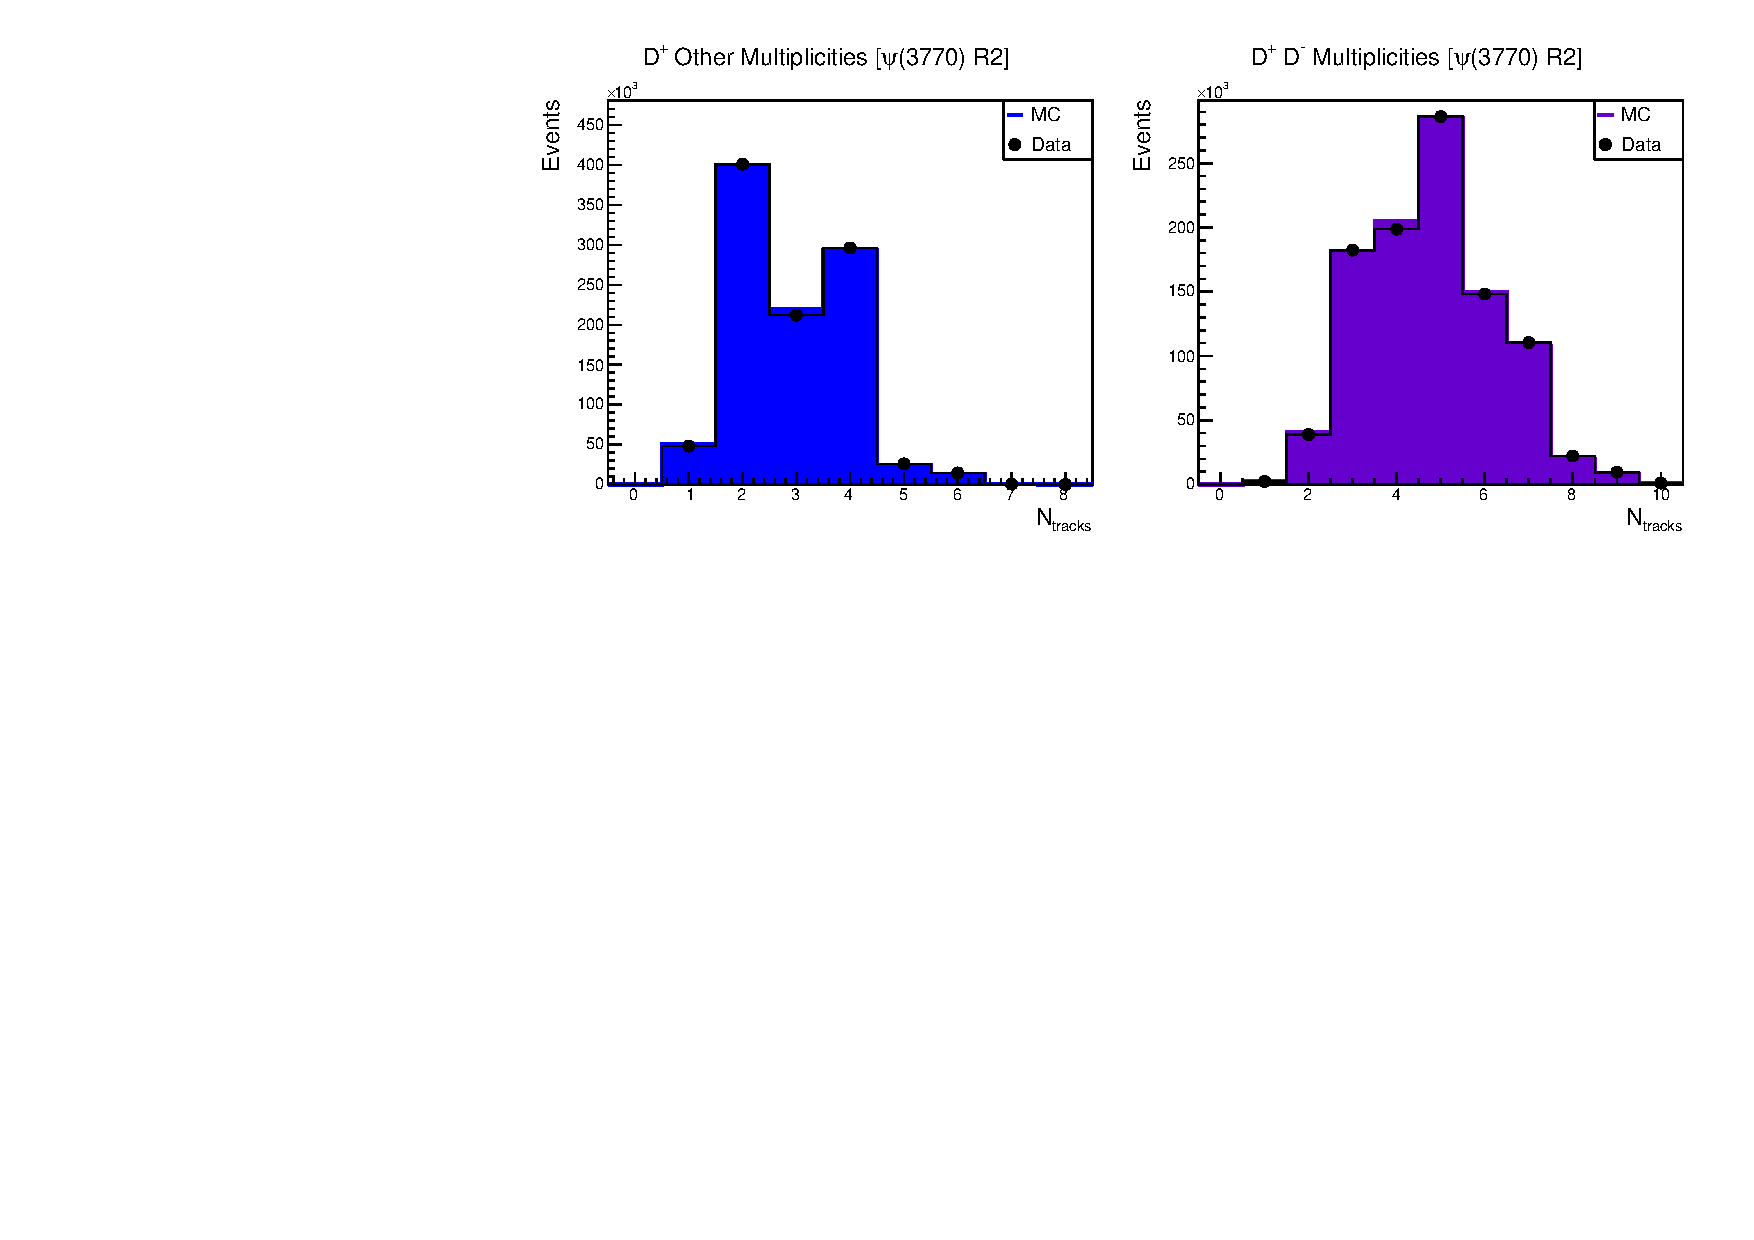
\includegraphics[scale=0.75]{figures/plots/DD_corr_plots/DD_psipp_DpDm_R2.pdf}
\caption{The other-side $\Dp$ tracks and corresponding $\Dp\Dm$ multiplicities for R2.}
{The distribution of good tracks not used for reconstruction of single-tagged $\Dp$ particles (left) is randomly sampled for pairs of points which comprise the convolved distribution (right).
The number of tracks in the $\Dp\Dm$ multiplicity distribution is used to determine the efficiency correction based off the cuts in \Cref{tab:DDbar_corr_cuts}.}
\label{fig:DD_corr_Dp_R2}
\end{figure}


\subsection{Reconstruction Efficiencies}
\label{ssec:nonDDbar_rec_efficiency_psipp}

MC samples for each of the new backgrounds introduced above the $\DDbar$ threshold were generated in the same way as for the continuum data.
The reconstruction efficiencies for each are shown in \Cref{tab:psipp_reconstruction}.
Values for the $\DO\aDO$ and $\Dp\Dm$ samples have already been multiplied by the correction factors discussed in \Cref{ssec:DDbar_correction}.

For the cross section of $\ypsip$, rather than the radiative return formula (as used with $\yjpsi$), we use results from CLEO-c and BESIII to determine the value.
These values are $\sigma(\ee \rightarrow \ypsip, \; \psip \rightarrow \pip \pim \jpsi) = (1036 \pm 13 \pm 23) \; \si{\pb}$ from the CLEO-c measurement, and $\Gamma(\psip \rightarrow \pip \pim \jpsi) = \SI{34.43 \pm 0.30}{\%}$ after averaging the BESIII measurement with the value from the PDG.
From this, we determine
\beq
\label{eq:ypsip_xsec}
\sigma(\ee \rightarrow \gamma\psi') = \frac{ \sigma(\ee \rightarrow \gamma\psi', \; \psi' \rightarrow \pip \pim \jpsi) }{ \Gamma(\psi' \rightarrow \pip \pim \jpsi) } = \SI{3009 \pm 81}{\pb}.
\eeq
Additionally, the $\DO\aDO$ and $\Dp\Dm$ cross sections are taken from the on-peak $\psipp$ measurement performed by Derrick Toth \cite{ref:Toth:2014}.


\begin{table}[H]
\centering
\renewcommand\arraystretch{1.0}

\begin{tabular}{c|r|cr@{$\; \pm \;$}rc cr@{$\; \pm \;$}rc cr@{$\; \pm \;$}rc}
\hline
\multicolumn{14}{c}{$\psipp$ (R1) Reconstruction} \\
\hline
Sample & $\sigma$ [\si{\nb}] & \multicolumn{4}{c}{$\effmc$ (SHAD) [\%]} & \multicolumn{4}{c}{$\effmc$ (LHAD) [\%]} & \multicolumn{4}{c}{$\effmc$ (THAD) [\%]} \\
\hline
$\DO\aDO$    & 3.615 && 73.9324 & 0.0142 &&& 79.8496 & 0.0147 &&& 60.3601 & 0.0128 & \\
$\Dp\Dm$     & 2.830 && 61.4048 & 0.0146 &&& 68.8212 & 0.0154 &&& 49.4007 & 0.0131 & \\
$\tautau$    & 2.652 && 12.7566 & 0.0253 &&& 28.0142 & 0.0374 &&&  9.8776 & 0.0222 & \\
$\yjpsi$     & 0.986 && 46.6185 & 0.0206 &&& 56.2494 & 0.0227 &&& 34.7544 & 0.0178 & \\
$\ypsip$     & 3.009 && 63.2551 & 0.0137 &&& 69.9696 & 0.0144 &&& 51.5643 & 0.0123 & \\
\hline          
\end{tabular}

\vspace{0.5cm}

\begin{tabular}{c|r|cr@{$\; \pm \;$}rc cr@{$\; \pm \;$}rc cr@{$\; \pm \;$}rc}
\hline
\multicolumn{14}{c}{$\psipp$ (R2) Reconstruction} \\
\hline
Sample & $\sigma$ [\si{\nb}] & \multicolumn{4}{c}{$\effmc$ (SHAD) [\%]} & \multicolumn{4}{c}{$\effmc$ (LHAD) [\%]} & \multicolumn{4}{c}{$\effmc$ (THAD) [\%]} \\
\hline
$\DO\aDO$    & 3.615 && 74.5111 & 0.0097 &&& 80.3399 & 0.0101 &&& 61.0386 & 0.0088 & \\
$\Dp\Dm$     & 2.830 && 61.8444 & 0.0100 &&& 69.1974 & 0.0106 &&& 49.9163 & 0.0090 & \\
$\tautau$    & 2.652 && 12.8646 & 0.0254 &&& 28.2140 & 0.0376 &&& 10.0198 & 0.0224 & \\
$\yjpsi$     & 0.986 && 47.0066 & 0.0146 &&& 56.6679 & 0.0161 &&& 35.1951 & 0.0127 & \\
$\ypsip$     & 3.009 && 63.7345 & 0.0097 &&& 70.4050 & 0.0102 &&& 52.1189 & 0.0088 & \\
\hline          
\end{tabular}

\caption{Reconstruction of background samples for the $\psipp$ data.}
\label{tab:psipp_reconstruction}
\end{table}

\pagebreak

\subsection{Signal Amounts}
\label{ssec:nonDDbar_signal_amounts_psipp}

Using the reconstruction efficiencies from \Cref{ssec:nonDDbar_rec_efficiency_psipp}, we can compute the contribution of background events for each sample.
For the $\qqbar$ component, we scale the number of hadronic events found in the 3650 (Old) sample based on \cref{eq:eff_extrapolation} for both R1 and R2 separately.
Due to the uncertainty on the extrapolation procedure, this becomes the dominant source of error on the resulting hadronic events.
This is also highly susceptible to the assumption of the $\psip$ shape for calculating the continuum points in the extrapolation fit.
The resulting number of hadronic events is shown in \Cref{tab:psipp_results}.

\begin{table}[H]
\centering
\renewcommand\arraystretch{1.0}

\begin{tabular}{c|cr@{$\; \pm \;$}rc cr@{$\; \pm \;$}rc cr@{$\; \pm \;$}rc}
\hline
\multicolumn{13}{c}{$\psipp$ (R1) Results} \\
\hline
Sample & \multicolumn{4}{c}{$\Nhad$ (SHAD)} & \multicolumn{4}{c}{$\Nhad$ (LHAD)} & \multicolumn{4}{c}{$\Nhad$ (THAD)} \\
\hline
Data             && 15694505 &  3962 &&& 17722728 &  4210 &&& 12580701 &  3547 & \\
$\qqbar^\dagger$ &&  8522688 & 71353 &&&  9330411 & 76320 &&&  6789405 & 61599 & \\
$\DO\aDO$        &&  2477345 &   534 &&&  2675620 &   560 &&&  2022561 &   473 & \\
$\Dp\Dm$         &&  1610764 &   414 &&&  1805311 &   442 &&&  1295875 &   366 & \\
$\tautau$        &&   313542 &   622 &&&   688559 &   922 &&&   242781 &   547 & \\
$\yjpsi$         &&   425891 &   193 &&&   513875 &   213 &&&   317504 &   166 & \\
$\ypsip$         &&  1764254 &   419 &&&  1951528 &   445 &&&  1438185 &   372 & \\
\hline                                                         
Hadrons          &&   490569 & 71795 &&&   658730 & 76807 &&&   401064 & 61995 & \\
\hline
\end{tabular}

\vspace{0.5cm}

\begin{tabular}{c|cr@{$\; \pm \;$}rc cr@{$\; \pm \;$}rc cr@{$\; \pm \;$}rc}
\hline
\multicolumn{13}{c}{$\psipp$ (R2) Results} \\
\hline
Sample & \multicolumn{4}{c}{$\Nhad$ (SHAD)} & \multicolumn{4}{c}{$\Nhad$ (LHAD)} & \multicolumn{4}{c}{$\Nhad$ (THAD)} \\
\hline
Data              && 33867464 &   5820 &&& 38217129 &   6182 &&& 27271529 &   5222 & \\
$\qqbar^\dagger$  && 18314683 & 154300 &&& 20015495 & 164688 &&& 14644571 & 133785 & \\
$\DO\aDO$         &&  5330375 &    738 &&&  5747352 &    770 &&&  4366577 &    662 & \\
$\Dp\Dm$          &&  3463499 &    583 &&&  3875291 &    620 &&&  2795485 &    520 & \\
$\tautau$         &&   675063 &   1331 &&&  1480514 &   1972 &&&   525781 &   1175 & \\
$\yjpsi$          &&   916819 &    288 &&&  1105253 &    317 &&&   686446 &    249 & \\
$\ypsip$          &&  3795113 &    603 &&&  4192317 &    636 &&&  3103459 &    541 & \\

\hline                                                         
Hadrons           &&  1179686 & 155135 &&&  1589187 & 165610 &&&   991049 & 134532 & \\
\hline
\end{tabular}

\caption{Hadronic events selected in the $\psipp$ data.}
{$^\dagger$ The $\qqbar$ contribution is obtained using an extrapolation from the continuum region in which the $\psip$ is assumed to have a standard Breit-Wigner shape.}
\label{tab:psipp_results}
\end{table}

\pagebreak


\subsection{Non-$\DDbar$ Branching Fraction (Breit-Wigner)}
\label{ssec:nonDDbar_bf_bw}

The resulting hadronic production is assumed to result from $\nonDDbar$ decays of the $\psipp$.
We can convert this into a cross section as follows:
\beq
\label{eq:nonDDbar_xsec}
\sigma(\psipptononDD) = \frac{ N_{\nonDDbar} }{ \epsilon_{\nonDDbar} \times \lum }.
\eeq
For the efficiency of $\nonDDbar$ events, the value of $\effmc$ for $\ypsip$ is used due to the assumption of similar behavior in their decays.
Using the standard Breit-Wigner assumption for the $\psip$, the results for the cross section and branching fraction of $\nonDDbar$ decays from $\psipp$ are shown in \Cref{tab:nonDDbar_xsec_psipp,tab:nonDDbar_bf_psipp}.

\begin{table}[H]
\centering
\renewcommand\arraystretch{1.0}
\begin{tabular}{c|cr@{$\; \pm \;$}rc cr@{$\; \pm \;$}rc cr@{$\; \pm \;$}rc}
\hline
Sample & \multicolumn{4}{c}{$\sigma_{\nonDDbar}$ [\si{\nb}] (SHAD)} & \multicolumn{4}{c}{$\sigma_{\nonDDbar}$ [\si{\nb}] (LHAD)} & \multicolumn{4}{c}{$\sigma_{\nonDDbar}$ [\si{\nb}] (THAD)} \\[1pt]
\hline
$\psipp$ (R1) && 0.9892 & 0.1219 &&& 1.1679 & 0.1179 &&& 0.9925 & 0.1291 & \\
$\psipp$ (R2) && 1.0877 & 0.1224 &&& 1.2926 & 0.1183 &&& 1.1142 & 0.1298 & \\
\hline                                                         
Lum. Weighted && 1.0563 & 0.1223 &&& 1.2528 & 0.1182 &&& 1.0754 & 0.1296 & \\ 
\hline
\end{tabular}
\caption{Cross sections for $\psipptononDD$ found using the $\psipp$ data.}
{The $\qqbar$ contributions were calculated using the Breit-Wigner formulation for the $\psip$ component in the continuum extrapolation.}
\label{tab:nonDDbar_xsec_psipp}
\end{table}

\begin{table}[H]
\centering
\renewcommand\arraystretch{1.0}
\begin{tabular}{c|cr@{$\; \pm \;$}rc cr@{$\; \pm \;$}rc cr@{$\; \pm \;$}rc}
\hline
Sample & \multicolumn{4}{c}{$\Gamma_{\nonDDbar}$ (SHAD)} & \multicolumn{4}{c}{$\Gamma_{\nonDDbar}$ (LHAD)} & \multicolumn{4}{c}{$\Gamma_{\nonDDbar}$ (THAD)} \\[1pt]
\hline
$\psipp$ (R1) && 0.1331 & 0.0183 &&& 0.1534 & 0.0185 &&& 0.1334 & 0.0190 & \\
$\psipp$ (R2) && 0.1444 & 0.0186 &&& 0.1671 & 0.0189 &&& 0.1474 & 0.0193 & \\
\hline                                                         
Lum. Weighted && 0.1408 & 0.0185 &&& 0.1627 & 0.0187 &&& 0.1430 & 0.0192 & \\ 
\hline
\end{tabular}
\caption{Branching fractions for $\psipptononDD$ found using the $\psipp$ data.}
{The $\qqbar$ contributions were calculated using the Breit-Wigner formulation for the $\psip$ component in the continuum extrapolation.}
\label{tab:nonDDbar_bf_psipp}
\end{table}

\pagebreak


\section{$\psip$ Background Investigation}
\label{sec:psip_background}

The most impactful assumption for the measurement of the branching fraction is the cross section shape of $\psip$ in the continuum region.
For the procedure thus far, we have assumed this shape to be a standard Breit-Wigner.
Given the drop in relative efficiency for the 3671 (New) data point (see \Cref{fig:extrapolation_SHAD}), it is likely this overestimates the branching fraction (see \Cref{tab:nonDDbar_bf_psipp}) by subtracting off too large of a background component for the $\psip$.

As an alternative comparison, we use the ratio of cross section productions for the resonance peak and continuum values,
\beq
\label{eq:psip_xsec_ratio}
\frac{ \sigma_{\text{res}} }{ \sigma_{\text{cont}}(\Ecm) } = \frac{ \sqrt{2\pi} \; (M_{\text{res}} - \Ecm)^2 }{ \Gamma_{\text{res}} \times \sigma_{\Ecm} },
\eeq
where $M_{\text{res}}$ and $\Gamma_{\text{res}}$ are the mass and total width of the resonance, respectively, and $\sigma_{\Ecm}$ is the center-of-mass energy spread during collection of the data.
For the $\psip$, with $M_{\psip} = \SI{3686.1}{\MeV}$ and $\Gamma_{\psip} = \SI{0.299}{\MeV}$, assuming an energy spread of $\sigma_{\Ecm} = \SI{1.5}{\MeV}$ gives $\sigma_{\psip} \sim 2500 \times \sigma_{\text{cont}}(\Ecm)$ at $\Ecm = \SI{3.665}{\GeV}$.

In 2009, BESIII collected \SI{166.25}{\invpb} of data at $\Ecm = \SI{3.686}{\GeV}$ and found $(106.41 \pm 0.86) \times 10^6$ events of $\psip$ decays \cite{ref:Ablikim:2013c}, corresponding to $\sigma_{\psip} \sim \SI{640}{\nb}$.
Using \Cref{eq:psip_xsec_ratio} for each of the continuum points, we obtain the cross section values shown in \Cref{tab:psip_xsec_ratio}, where each generally is notably smaller than from the Breit-Wigner assumption.

\begin{table}[H]
\centering
\renewcommand\arraystretch{1.0}
\begin{tabular}{c|c|c c}
\hline
Sample & $\Ecm$ [\si{\GeV}] & $\sigma_{\psip}$ [\si{\nb}] (Ratio) & $\sigma_{\psip}$ [\si{\nb}] (BW) \\
\hline
3500 (New) & 3.496 & 0.0032 & 0.0056 \\
3542 (New) & 3.538 & 0.0052 & 0.0092 \\
3600 (New) & 3.596 & 0.0141 & 0.0244 \\
3650 (New) & 3.644 & 0.0646 & 0.1101 \\
3671 (New) & 3.665 & 0.2572 & 0.4359 \\
3650 (Old) & 3.650 & 0.0879 & 0.1495 \\
\hline                                                         
\end{tabular}
\caption{Cross sections of $\psip$ calculated using two different methods.}
\label{tab:psip_xsec_ratio}
\end{table}


\subsection{Non-$\DDbar$ Branching Fraction ($\psip$ from Data)}
\label{ssec:nonDDbar_bf_calc}

We repeat the procedure using the cross sections calculated based off \Cref{eq:psip_xsec_ratio} in place of the Breit-Wigner values (see \Cref{tab:psip_xsec_ratio}).
This leads to the continuum extrapolations shown in \Cref{fig:extrapolation_SHAD_ratio,fig:extrapolation_LHAD_ratio,fig:extrapolation_THAD_ratio}.
The $\nonDDbar$ results are shown in \Cref{tab:nonDDbar_xsec_psipp_calc,tab:nonDDbar_bf_psipp_calc}, where the branching fractions are lower on average by around 1.6\% compared to the original method.

\begin{table}[H]
\centering
\renewcommand\arraystretch{1.0}
\begin{tabular}{c|cr@{$\; \pm \;$}rc cr@{$\; \pm \;$}rc cr@{$\; \pm \;$}rc}
\hline
Sample & \multicolumn{4}{c}{$\sigma_{\nonDDbar}$ [\si{\nb}] (SHAD)} & \multicolumn{4}{c}{$\sigma_{\nonDDbar}$ [\si{\nb}] (LHAD)} & \multicolumn{4}{c}{$\sigma_{\nonDDbar}$ [\si{\nb}] (THAD)} \\[1pt]
\hline
$\psipp$ (R1) && 0.8367 & 0.1224 &&& 1.0157 & 0.1184 &&& 0.8391 & 0.1297 & \\
$\psipp$ (R2) && 0.9353 & 0.1230 &&& 1.1406 & 0.1189 &&& 0.9609 & 0.1304 & \\
\hline                                                         
Lum. Weighted && 0.9039 & 0.1228 &&& 1.1008 & 0.1187 &&& 0.9220 & 0.1302 & \\ 
\hline
\end{tabular}
\caption{Cross sections for $\psipptononDD$ found using the $\psipp$ data.}
{The $\qqbar$ contributions were calculated using $\psip$ data for the $\psip$ components in the continuum extrapolation.}
\label{tab:nonDDbar_xsec_psipp_calc}
\end{table}

\begin{table}[H]
\centering
\renewcommand\arraystretch{1.0}
\begin{tabular}{c|cr@{$\; \pm \;$}rc cr@{$\; \pm \;$}rc cr@{$\; \pm \;$}rc}
\hline
Sample & \multicolumn{4}{c}{$\Gamma_{\nonDDbar}$ (SHAD)} & \multicolumn{4}{c}{$\Gamma_{\nonDDbar}$ (LHAD)} & \multicolumn{4}{c}{$\Gamma_{\nonDDbar}$ (THAD)} \\[1pt]
\hline
$\psipp$ (R1) && 0.1149 & 0.0180 &&& 0.1361 & 0.0181 &&& 0.1152 & 0.0188 & \\
$\psipp$ (R2) && 0.1267 & 0.0183 &&& 0.1504 & 0.0185 &&& 0.1297 & 0.0190 & \\
\hline                                                         
Lum. Weighted && 0.1230 & 0.0182 &&& 0.1458 & 0.0183 &&& 0.1251 & 0.0190 & \\ 
\hline
\end{tabular}
\caption{Branching fractions for $\psipptononDD$ found using the $\psipp$ data.}
{The $\qqbar$ contributions were calculated using $\psip$ data for the $\psip$ components in the continuum extrapolation.}
\label{tab:nonDDbar_bf_psipp_calc}
\end{table}

\begin{figure}[H]
\centering
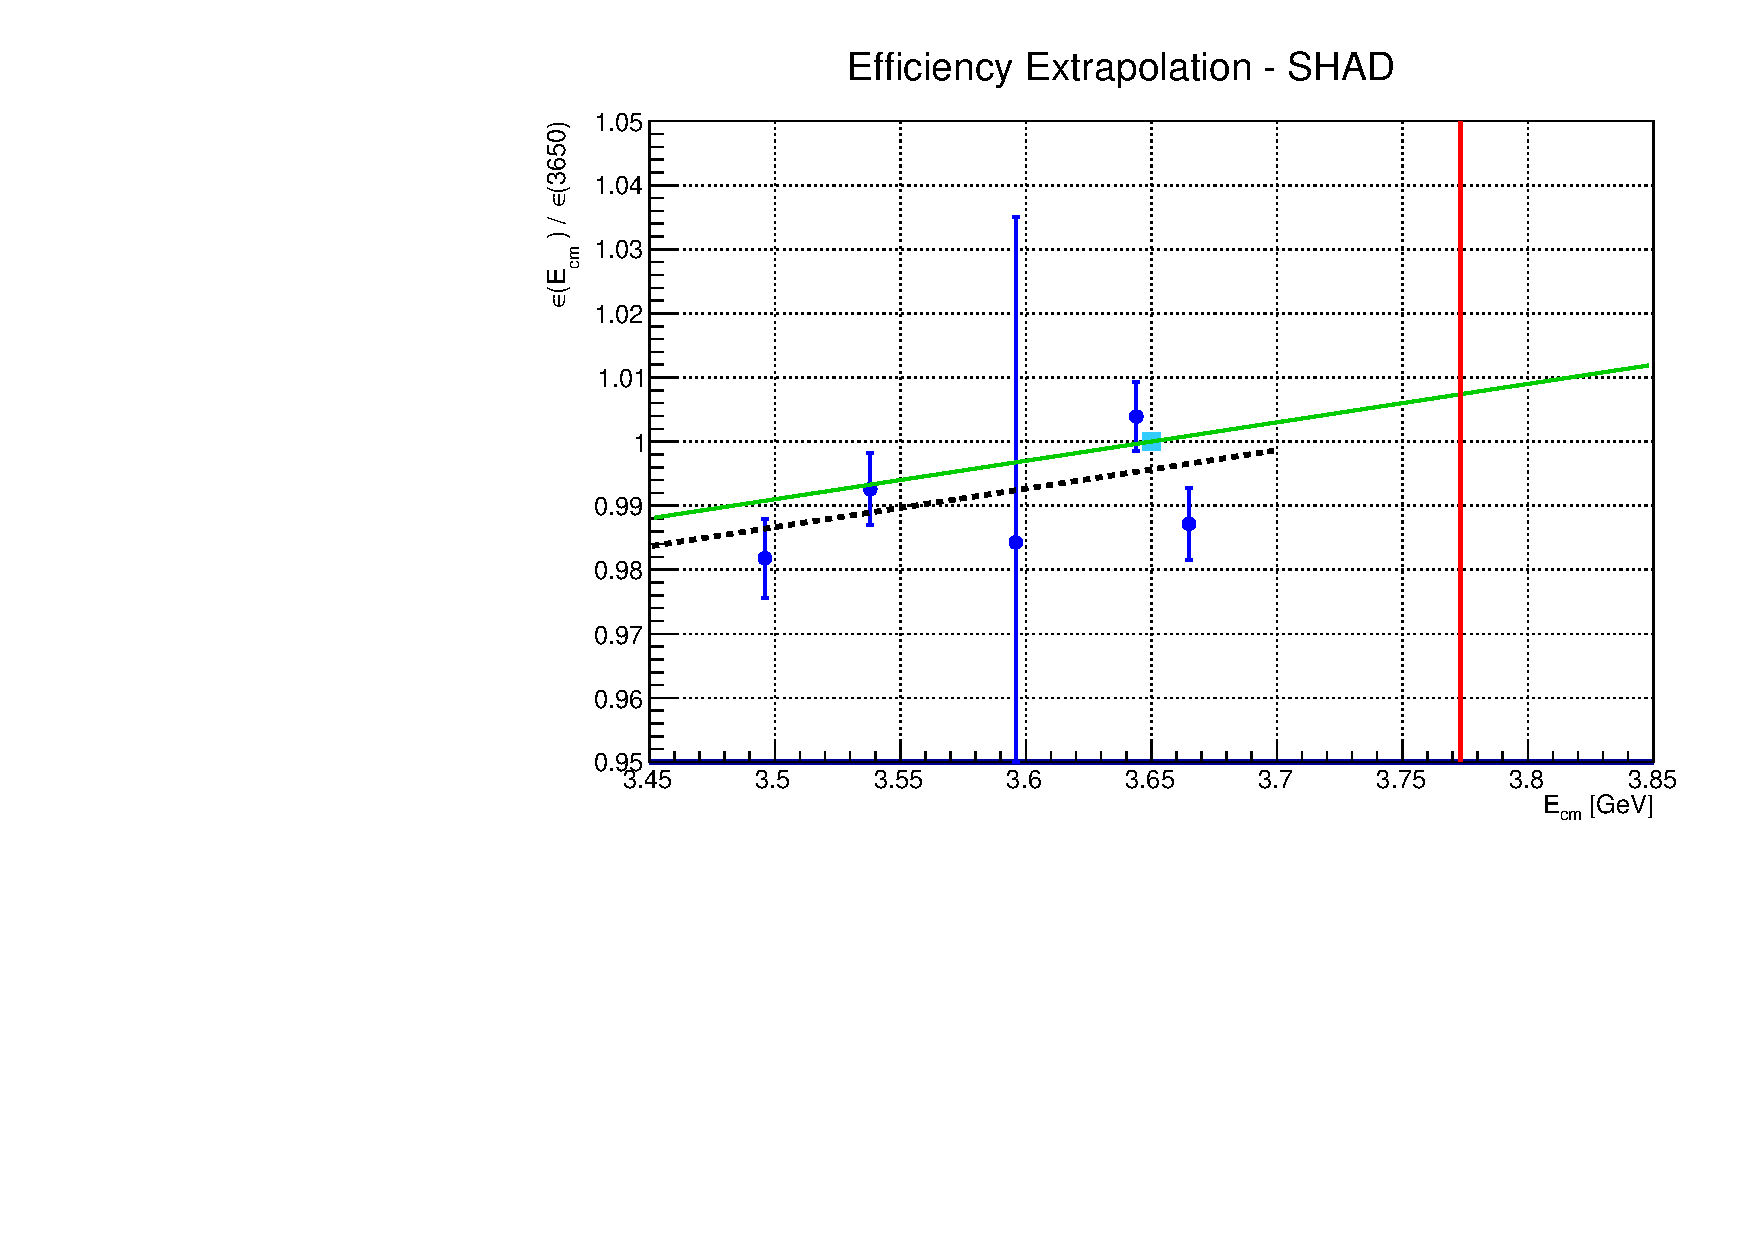
\includegraphics[scale=0.75]{figures/plots/SHAD_psip_calc.pdf}
\caption{The extrapolation for SHAD events using $\psip$ data.}
{The new continuum points (blue) are fit using a linear slope (dashed black), then extrapolated to higher energies (solid green) based on the old continuum energy point at \SI{3.650}{\GeV} (cyan).
 The energy point for the $\psipp$ samples at \SI{3.773}{\GeV} is also shown (solid red).}
\label{fig:extrapolation_SHAD_ratio}
\end{figure}

\begin{figure}[H]
\centering
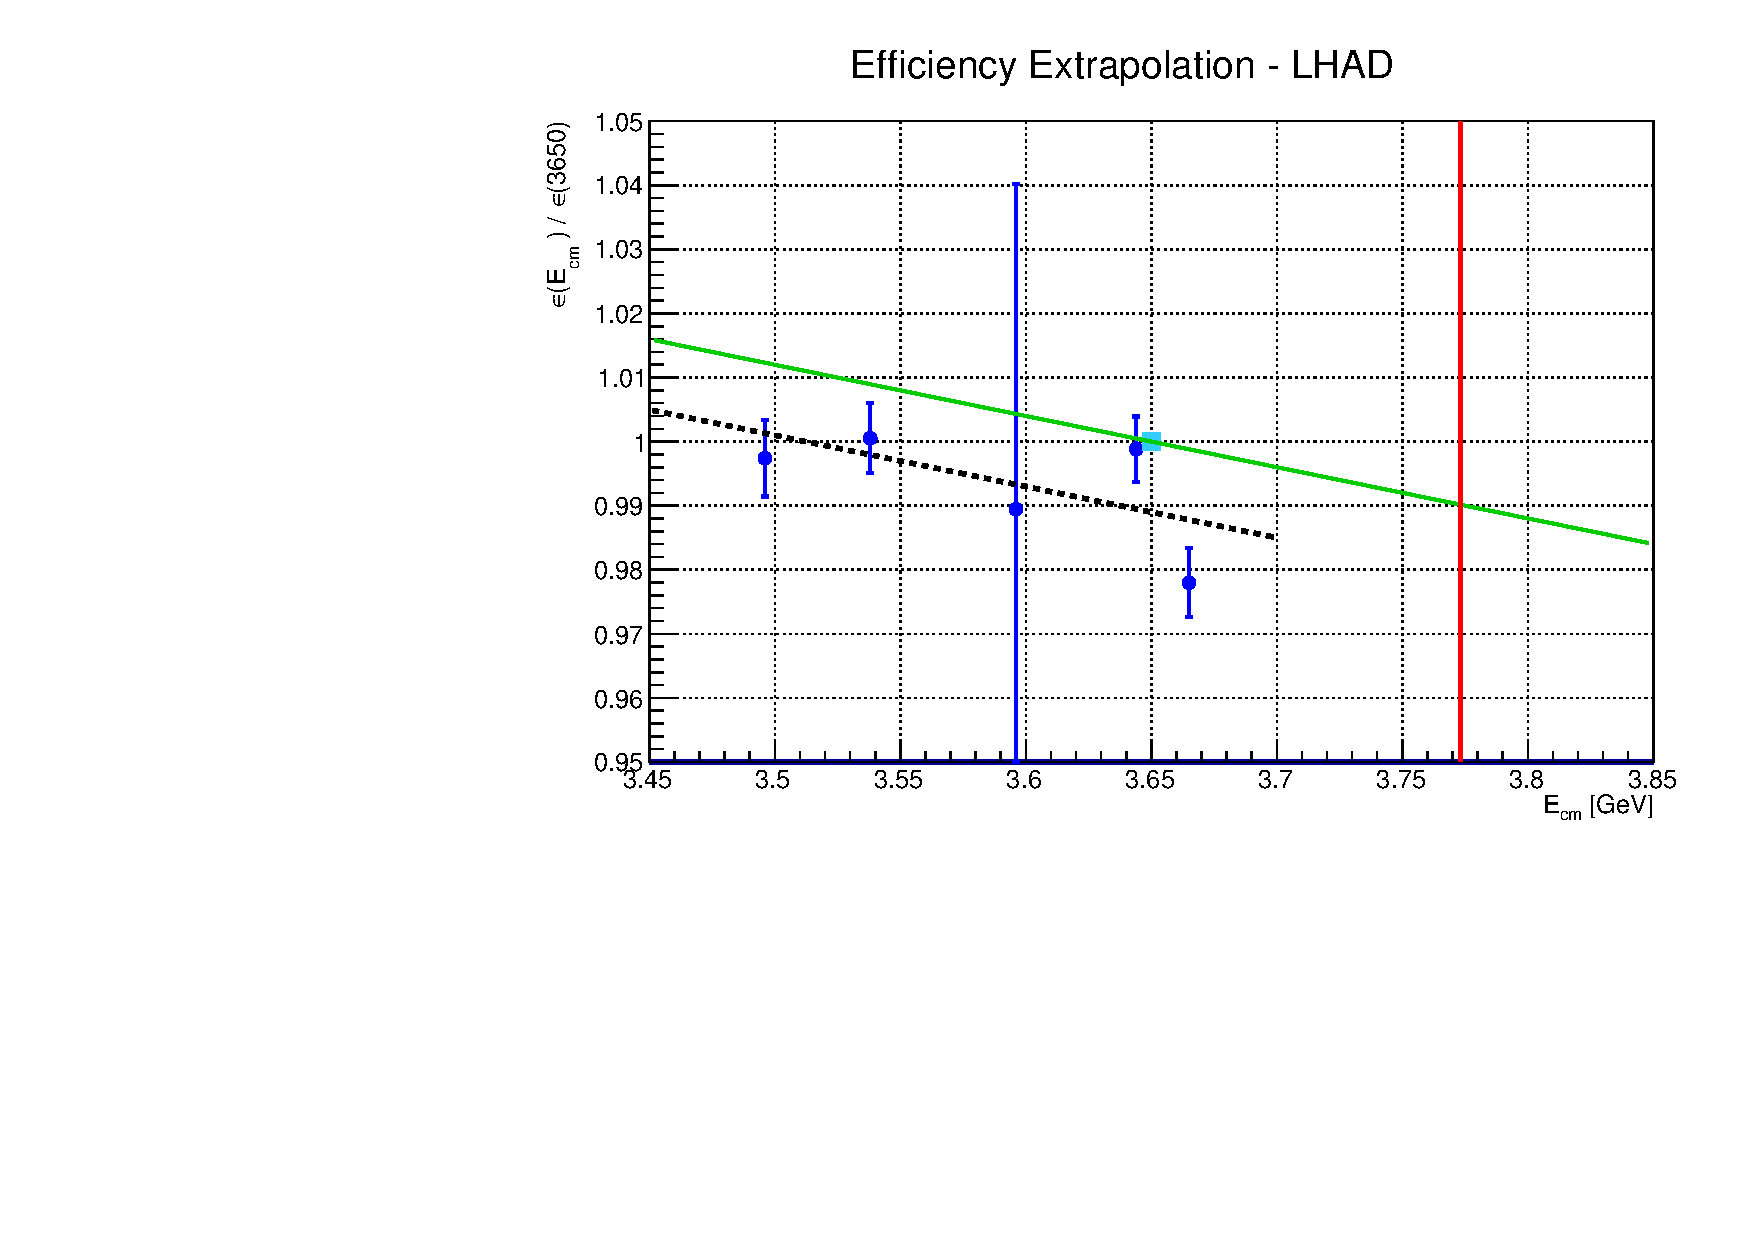
\includegraphics[scale=0.75]{figures/plots/LHAD_psip_calc.pdf}
\caption{The extrapolation for LHAD events using $\psip$ data.}
{The new continuum points (blue) are fit using a linear slope (dashed black), then extrapolated to higher energies (solid green) based on the old continuum energy point at \SI{3.650}{\GeV} (cyan).
 The energy point for the $\psipp$ samples at \SI{3.773}{\GeV} is also shown (solid red).}
\label{fig:extrapolation_LHAD_ratio}
\end{figure}

\begin{figure}[H]
\centering
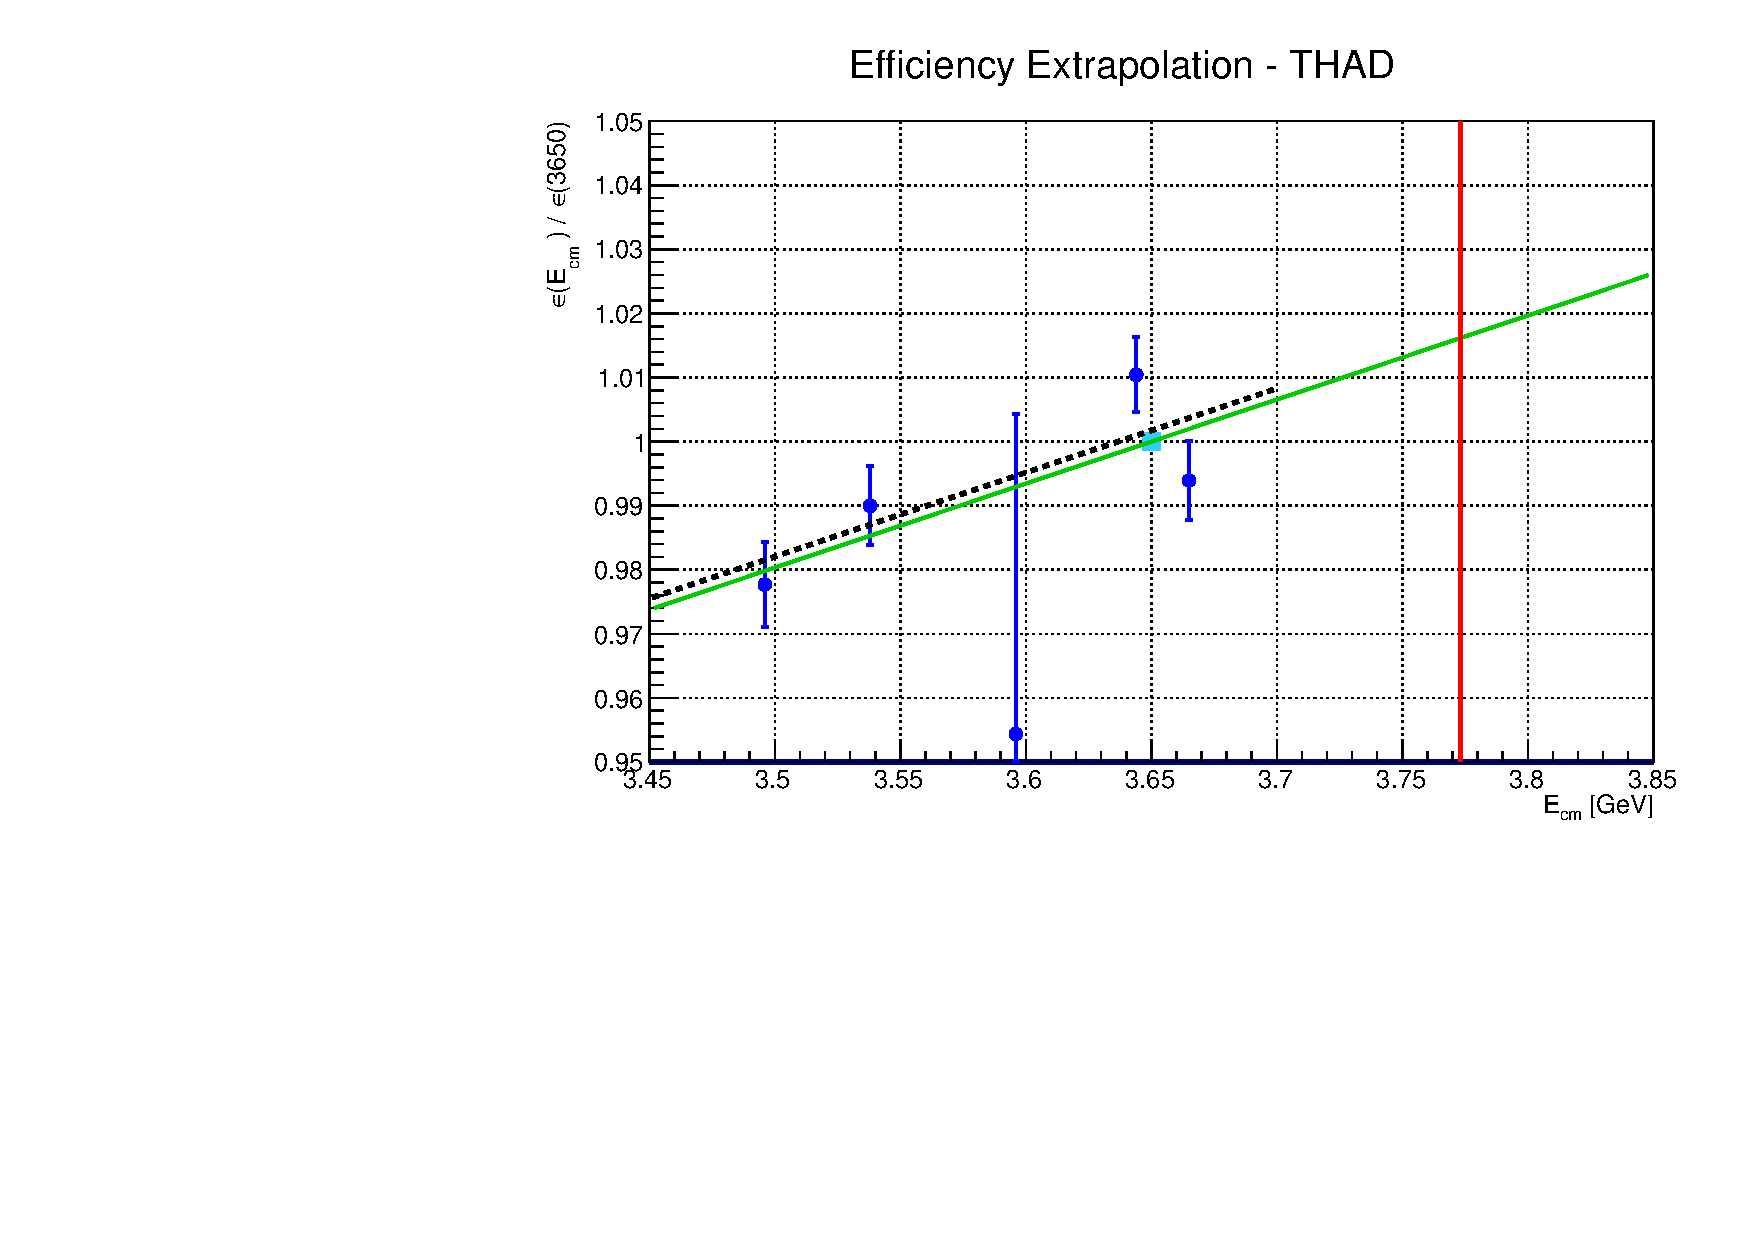
\includegraphics[scale=0.75]{figures/plots/THAD_psip_calc.pdf}
\caption{The extrapolation for THAD events using $\psip$ data.}
{The new continuum points (blue) are fit using a linear slope (dashed black), then extrapolated to higher energies (solid green) based on the old continuum energy point at \SI{3.650}{\GeV} (cyan).
 The energy point for the $\psipp$ samples at \SI{3.773}{\GeV} is also shown (solid red).}
\label{fig:extrapolation_THAD_ratio}
\end{figure}

\pagebreak

\subsection{Non-$\DDbar$ Branching Fraction ($\psip$ Excluded)}
\label{ssec:nonDDbar_bf_none}

While the Breit-Wigner formulation likely provides an upper bound to the $\nonDDbar$ branching fractions, it is unclear how much lower the true values are.
The modification detailed in \Cref{sec:psip_background} provides a likely estimation of the actual value, but previous experiments have measured wildly fluctuating values.
In fact, some results have shown no evidence of a $\nonDDbar$ branching fraction at all.
To obtain a potential lower bound from our procedure, we can repeat the measurement without including any contribution from $\psip$ events.
This will increase the extrapolated reconstruction efficiency fits, which subtracts off a larger amount of hadrons from the $\psipp$ data, and corresponds to a lower branching fraction.
The results for this procedure are shown in \Cref{tab:nonDDbar_xsec_psipp_none,tab:nonDDbar_bf_psipp_none}.

\begin{table}[H]
\centering
\renewcommand\arraystretch{1.0}
\begin{tabular}{c|cr@{$\; \pm \;$}rc cr@{$\; \pm \;$}rc cr@{$\; \pm \;$}rc}
\hline
Sample & \multicolumn{4}{c}{$\sigma_{\nonDDbar}$ [\si{\nb}] (SHAD)} & \multicolumn{4}{c}{$\sigma_{\nonDDbar}$ [\si{\nb}] (LHAD)} & \multicolumn{4}{c}{$\sigma_{\nonDDbar}$ [\si{\nb}] (THAD)} \\[1pt]
\hline
$\psipp$ (R1) && 0.6190 & 0.1232 &&& 0.7986 & 0.1192 &&& 0.6203 & 0.1305 & \\
$\psipp$ (R2) && 0.7179 & 0.1238 &&& 0.9239 & 0.1197 &&& 0.7421 & 0.1313 & \\
\hline                                                         
Lum. Weighted && 0.6864 & 0.1236 &&& 0.8839 & 0.1195 &&& 0.7033 & 0.1311 & \\ 
\hline
\end{tabular}
\caption{Cross sections for $\psipptononDD$ found using the $\psipp$ data.}
{The $\qqbar$ contributions were calculated after excluding the $\psip$ components in the continuum extrapolation.}
\label{tab:nonDDbar_xsec_psipp_none}
\end{table}

\begin{table}[H]
\centering
\renewcommand\arraystretch{1.0}
\begin{tabular}{c|cr@{$\; \pm \;$}rc cr@{$\; \pm \;$}rc cr@{$\; \pm \;$}rc}
\hline
Sample & \multicolumn{4}{c}{$\Gamma_{\nonDDbar}$ (SHAD)} & \multicolumn{4}{c}{$\Gamma_{\nonDDbar}$ (LHAD)} & \multicolumn{4}{c}{$\Gamma_{\nonDDbar}$ (THAD)} \\[1pt]
\hline
$\psipp$ (R1) && 0.0876 & 0.0178 &&& 0.1102 & 0.0176 &&& 0.0878 & 0.0187 & \\
$\psipp$ (R2) && 0.1002 & 0.0180 &&& 0.1254 & 0.0179 &&& 0.1033 & 0.0188 & \\
\hline                                                         
Lum. Weighted && 0.0962 & 0.0179 &&& 0.1205 & 0.0178 &&& 0.0983 & 0.0188 & \\
 \hline
\end{tabular}
\caption{Branching fractions for $\psipptononDD$ found using the $\psipp$ data.}
{The $\qqbar$ contributions were calculated after excluding the $\psip$ components in the continuum extrapolation.}
\label{tab:nonDDbar_bf_psipp_none}
\end{table}

\begin{figure}[H]
\centering
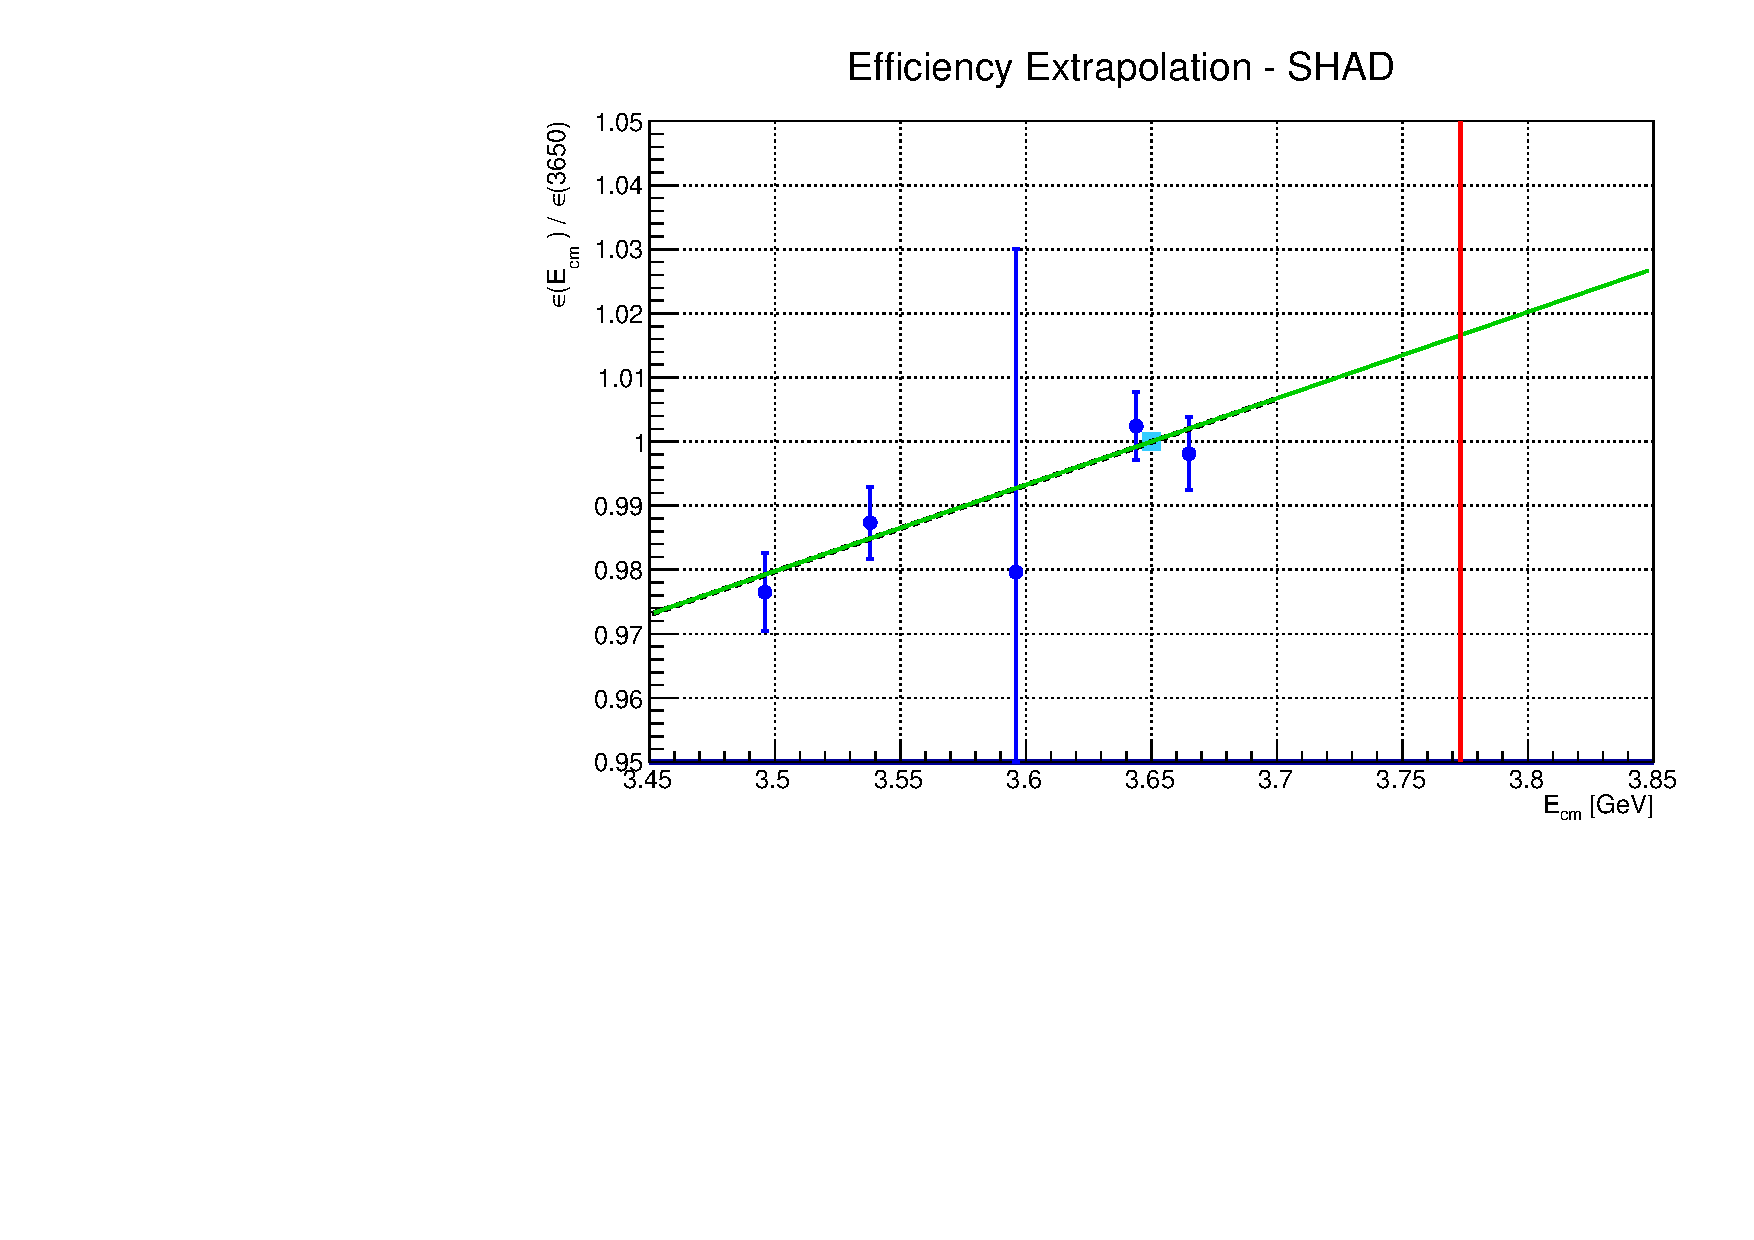
\includegraphics[scale=0.75]{figures/plots/SHAD_psip_none.pdf}
\caption{The extrapolation for SHAD events without including $\psip$ events.}
{The new continuum points (blue) are fit using a linear slope (dashed black), then extrapolated to higher energies (solid green) based on the old continuum energy point at \SI{3.650}{\GeV} (cyan).
 The energy point for the $\psipp$ samples at \SI{3.773}{\GeV} is also shown (solid red).}
\label{fig:extrapolation_SHAD_none}
\end{figure}

\begin{figure}[H]
\centering
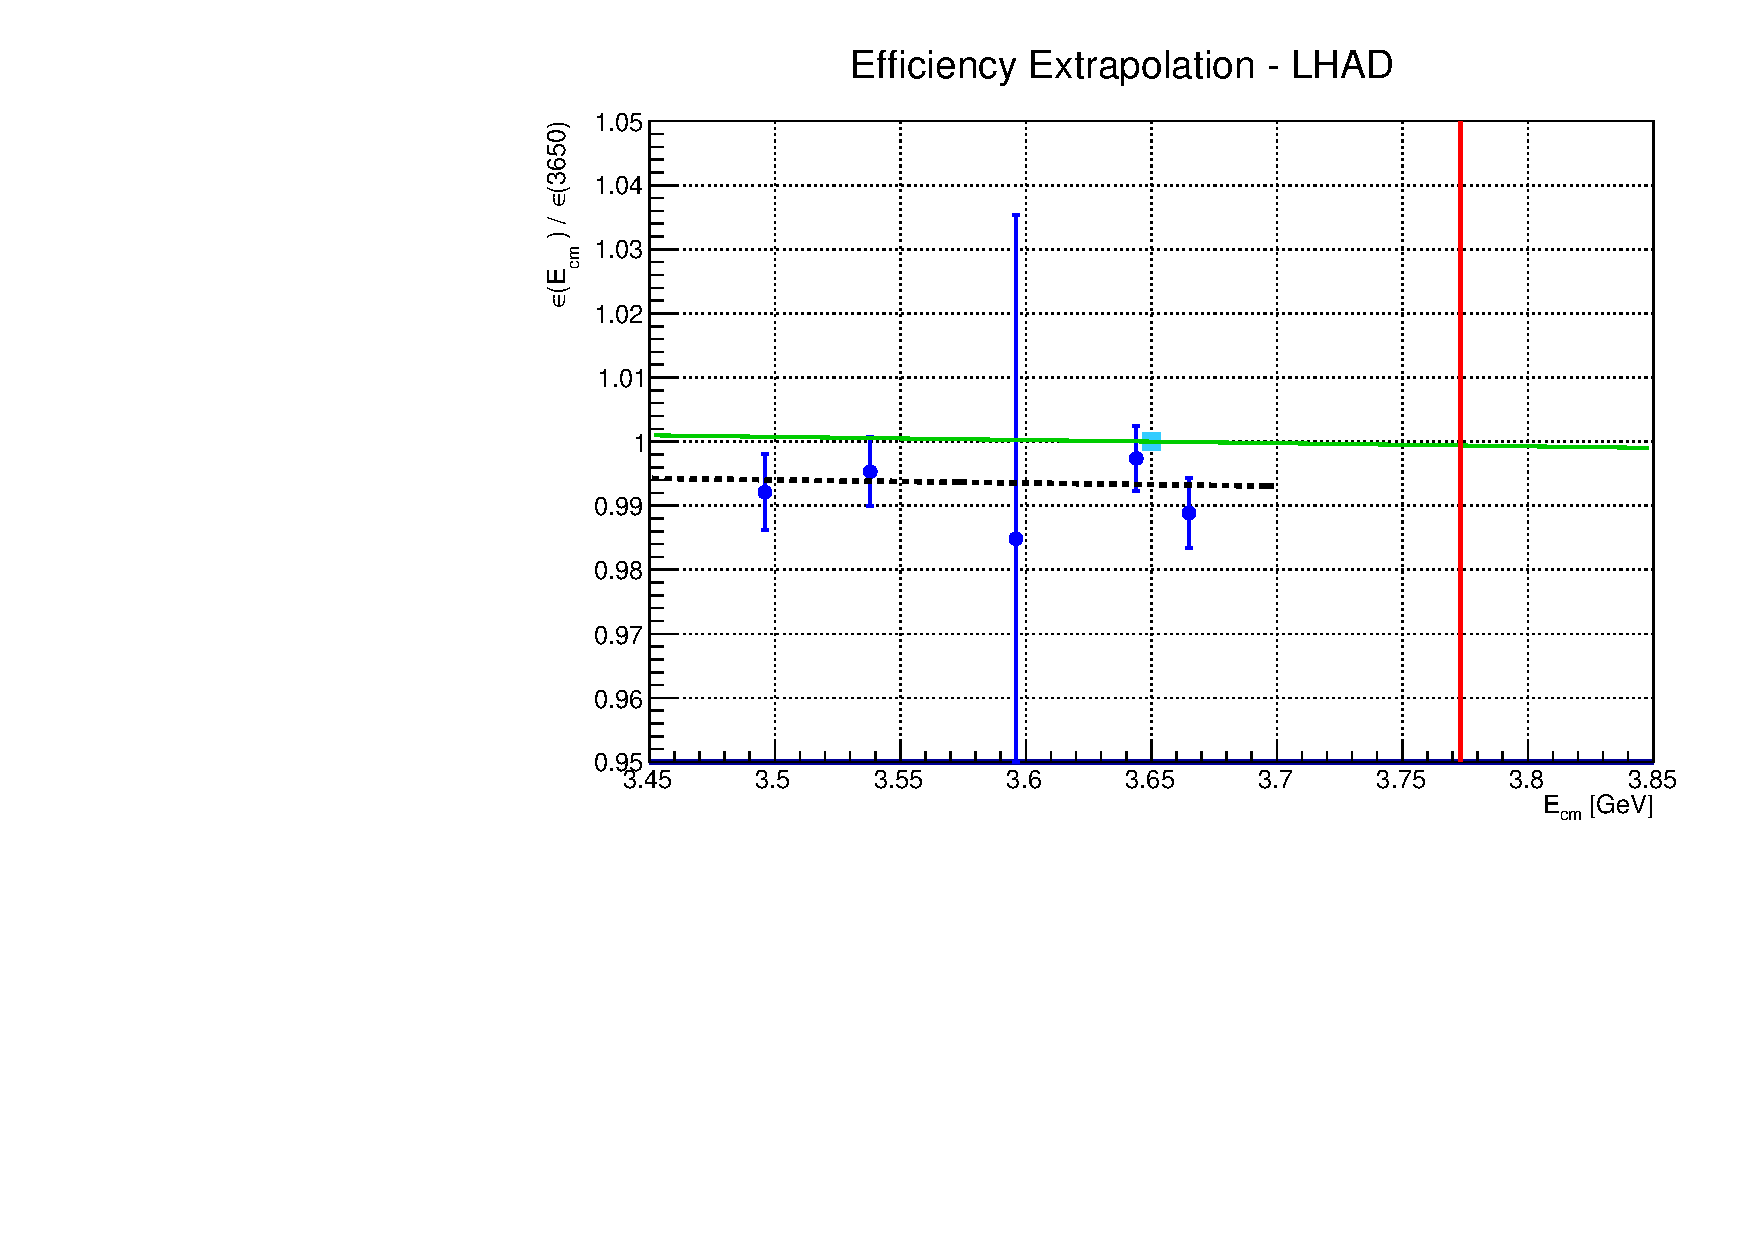
\includegraphics[scale=0.75]{figures/plots/LHAD_psip_none.pdf}
\caption{The extrapolation for LHAD events without including $\psip$ events.}
{The new continuum points (blue) are fit using a linear slope (dashed black), then extrapolated to higher energies (solid green) based on the old continuum energy point at \SI{3.650}{\GeV} (cyan).
 The energy point for the $\psipp$ samples at \SI{3.773}{\GeV} is also shown (solid red).}
\label{fig:extrapolation_LHAD_none}
\end{figure}

\begin{figure}[H]
\centering
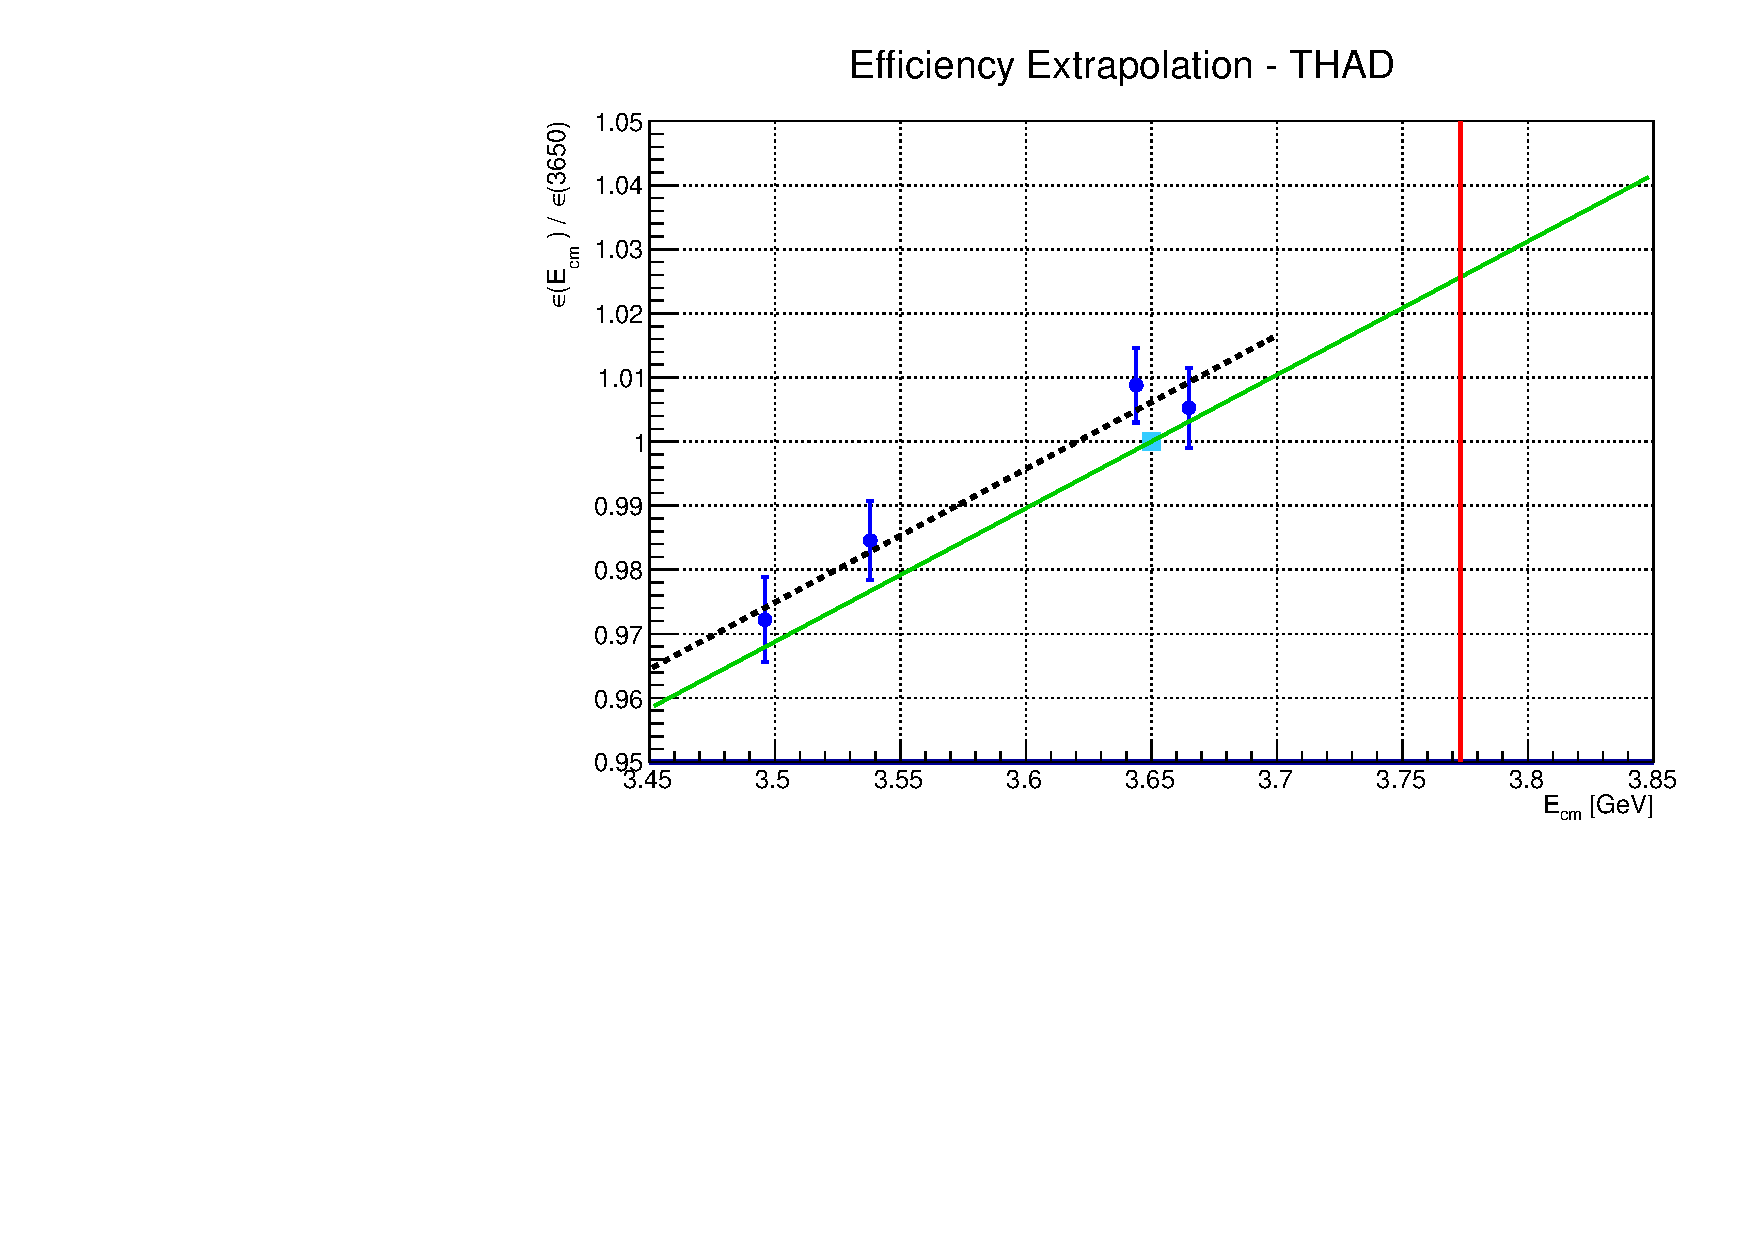
\includegraphics[scale=0.75]{figures/plots/THAD_psip_none.pdf}
\caption{The extrapolation for THAD events without including $\psip$ events.}
{The new continuum points (blue) are fit using a linear slope (dashed black), then extrapolated to higher energies (solid green) based on the old continuum energy point at \SI{3.650}{\GeV} (cyan).
 The energy point for the $\psipp$ samples at \SI{3.773}{\GeV} is also shown (solid red).}
\label{fig:extrapolation_THAD_none}
\end{figure}

\pagebreak


\section{Results for Scan Data}
\label{sec:non_DDbar_results_scan}

In addition to the $\psipp$ data, we also examine the energy points of the scan data.
While the statistics for these points are far lower, it will provide insight for the behavior of hadronic production with changing center-of-mass energy.
We use $\psip$ data in order to extrapolate the $\qqbar$ events throughout this region (see \Cref{ssec:nonDDbar_bf_calc}).

Each scan data point used will be referred to by its name listed in \Cref{tab:nonDDbar_scan_data}.
The cross sections for each background sample are also listed, where the $\DDbar$ values are taken from the results in \Cref{tab:xsec_rc_data_sys}.
To determine the cross sections of $\ypsip$ at each point, the values were calculated using the standard radiative formula (as for $\yjpsi$), then scaled by the ratio of the data-driven value from \Cref{eq:ypsip_xsec} to the value of this formula at \SI{3.773}{\GeV}.

The total hadronic counting fits for the scan data can be found in \Cref{app:nonDDbar_hadron_counts_scan}.
As the $\psipp$ R1 data was taken at a similar time as the scan data, we use the same $\DDbar$ corrections from R1 for all of the scan data sample points.
The reconstruction efficiencies and signal amounts can be found in \Cref{app:nonDDbar_rec_efficiency_scan,app:nonDDbar_signal_scan}, respectively.

In addition to the $\nonDDbar$ branching fraction, we can also examine the inclusive hadronic cross section as a function of center-of-mass energy:
Dividing the fit counts for each selection method from \Cref{app:nonDDbar_hadron_counts_scan} by the luminosities from \Cref{tab:luminosity}, we find the inclusive cross sections shown in \Cref{fig:xsec_inclusive_scan}.
As these values are independent of the extrapolation procedure, they are immediately ready for use in future analyses.

The $\nonDDbar$ cross sections and branching ratios calculated for each scan point are shown in \Cref{fig:xsec_nonDDbar_scan,fig:bf_nonDDbar_scan}, respectively.
For comparison, the same calculation for the $\psipp$ data is also shown on each of these plots.
Due to the uncertain cross section shape of the $\psip$ required to properly extrapolate to the scan data region, these values are not representative of a true measurement for the branching fraction.
For now, we have done our best to ensure the accuracy of all other background components analyzed.
This means, with an improved understanding of the $\psip$ cross section in the continuum region (likely to be analyzed in the very near future, as BESIII has data taking planned for this region), the branching fraction value can easily be updated for a final result.
From our analysis of the $\psip$ background (see \Cref{sec:psip_background}), we expect this value to be in the range \SIrange{9.6}{14.1}{\%} with our current estimate being \SI{12.3}{\%}.


\begin{table}[H]
\centering
\renewcommand\arraystretch{1.0}
\begin{tabular}{c|c|c c c c c}
\hline
Sample & $\Ecm$ [\si{\GeV}] & $\DO\aDO$ [\si{\nb}] & $\Dp\Dm$ [\si{\nb}] & $\tautau$ [\si{\nb}] & $\yjpsi$ [\si{\nb}] & $\ypsip$ [\si{\nb}] \\
\hline
3734 (Scan) & 3.7342 & 0.164 & 0.000 & 2.467 & 1.060 & 5.359 \\
3736 (Scan) & 3.7368 & 0.218 & 0.000 & 2.475 & 1.055 & 5.094 \\
3744 (Scan) & 3.7447 & 0.765 & 0.150 & 2.514 & 1.039 & 4.428 \\
3748 (Scan) & 3.7483 & 0.838 & 0.360 & 2.522 & 1.032 & 4.180 \\
3750 (Scan) & 3.7501 & 0.968 & 0.439 & 2.533 & 1.029 & 4.065 \\
3751 (Scan) & 3.7517 & 1.237 & 0.574 & 2.542 & 1.025 & 3.969 \\
3753 (Scan) & 3.7534 & 1.377 & 0.748 & 2.553 & 1.022 & 3.871 \\
3755 (Scan) & 3.7556 & 1.566 & 0.797 & 2.562 & 1.018 & 3.752 \\
3756 (Scan) & 3.7562 & 1.629 & 0.914 & 2.573 & 1.017 & 3.721 \\
3759 (Scan) & 3.7592 & 1.948 & 1.192 & 2.584 & 1.011 & 3.572 \\
3762 (Scan) & 3.7624 & 2.385 & 1.534 & 2.598 & 1.005 & 3.426 \\
3765 (Scan) & 3.7650 & 2.715 & 1.882 & 2.613 & 1.000 & 3.315 \\
3767 (Scan) & 3.7676 & 3.102 & 2.200 & 2.627 & 0.995 & 3.212 \\
3771 (Scan) & 3.7713 & 3.406 & 2.634 & 2.641 & 0.989 & 3.075 \\
3774 (Scan) & 3.7742 & 3.714 & 3.067 & 2.656 & 0.983 & 2.975 \\
3777 (Scan) & 3.7775 & 3.692 & 3.078 & 2.669 & 0.978 & 2.870 \\
3780 (Scan) & 3.7802 & 3.444 & 2.599 & 2.683 & 0.973 & 2.788 \\
3782 (Scan) & 3.7829 & 2.791 & 2.206 & 2.696 & 0.968 & 2.712 \\
3786 (Scan) & 3.7869 & 1.995 & 1.627 & 2.709 & 0.961 & 2.605 \\
3789 (Scan) & 3.7891 & 1.361 & 1.178 & 2.722 & 0.957 & 2.550 \\
3792 (Scan) & 3.7926 & 0.920 & 0.680 & 2.739 & 0.951 & 2.467 \\
3797 (Scan) & 3.7970 & 0.562 & 0.414 & 2.755 & 0.944 & 2.370 \\
3800 (Scan) & 3.8003 & 0.424 & 0.241 & 2.771 & 0.938 & 2.301 \\
3802 (Scan) & 3.8024 & 0.325 & 0.236 & 2.784 & 0.935 & 2.260 \\
3807 (Scan) & 3.8070 & 0.352 & 0.289 & 2.795 & 0.927 & 2.174 \\
3809 (Scan) & 3.8093 & 0.233 & 0.132 & 2.807 & 0.923 & 2.133 \\
3813 (Scan) & 3.8135 & 0.060 & 0.153 & 2.819 & 0.917 & 2.063 \\
3815 (Scan) & 3.8153 & 0.056 & 0.089 & 2.829 & 0.914 & 2.034 \\
3822 (Scan) & 3.8229 & 0.140 & 0.197 & 2.859 & 0.902 & 1.920 \\
3832 (Scan) & 3.8320 & 0.069 & 0.046 & 2.887 & 0.888 & 1.799 \\
3839 (Scan) & 3.8390 & 0.237 & 0.254 & 2.914 & 0.877 & 1.716 \\
3849 (Scan) & 3.8494 & 0.186 & 0.186 & 2.939 & 0.862 & 1.604 \\
3855 (Scan) & 3.8555 & 0.337 & 0.273 & 2.967 & 0.853 & 1.545 \\
3863 (Scan) & 3.8632 & 0.340 & 0.099 & 2.988 & 0.843 & 1.476 \\
\hline
\end{tabular}
\caption{Energy values and background cross sections for the scan data.}
\label{tab:nonDDbar_scan_data}
\end{table}

\begin{figure}[H]
\centering
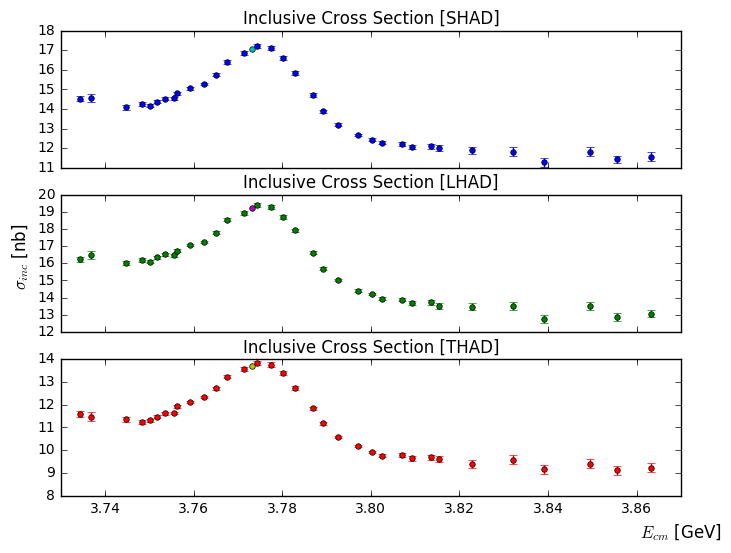
\includegraphics[scale=0.75]{figures/plots/xsec_inclusive_scan.png}
\caption{The inclusive cross sections measured for the scan data region.}
{The cyan, purple, and yellow points correspond to the luminosity-averaged inclusive cross sections measured for the $\psipp$ data.}
\label{fig:xsec_inclusive_scan}
\end{figure}

\begin{figure}[H]
\centering
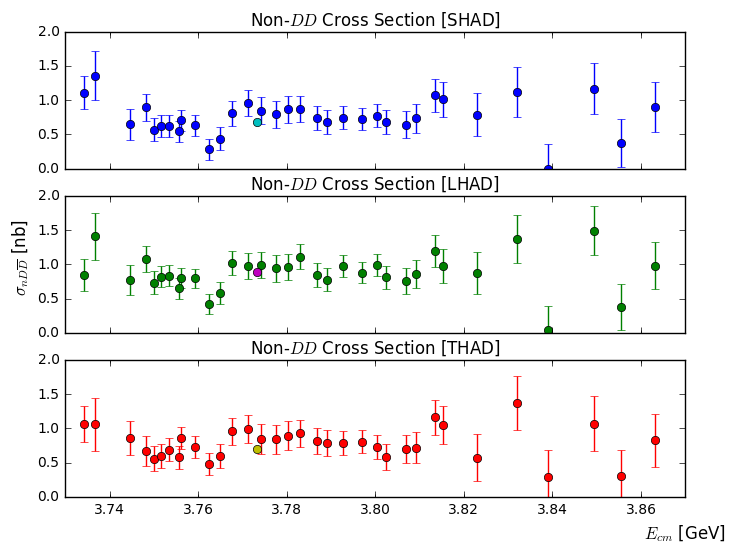
\includegraphics[scale=0.75]{figures/plots/xsec_nonDDbar_scan.png}
\caption{The $\nonDDbar$ cross sections measured for the scan data region.}
{The cyan, purple, and yellow points correspond to the luminosity-averaged $\nonDDbar$ cross sections measured for the $\psipp$ data.}
\label{fig:xsec_nonDDbar_scan}
\end{figure}

\begin{figure}[H]
\centering
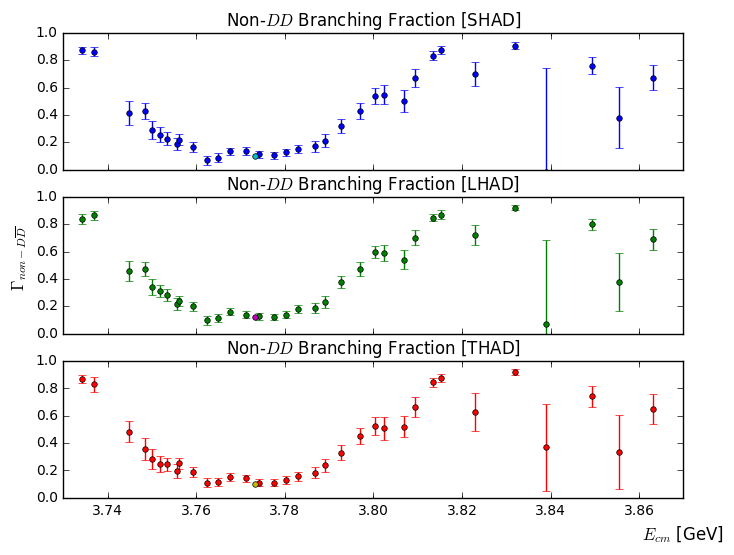
\includegraphics[scale=0.75]{figures/plots/bf_nonDDbar_scan.png}
\caption{The $\nonDDbar$ branching fractions measured for the scan data region.}
{The cyan, purple, and yellow points correspond to the luminosity-averaged $\nonDDbar$ branching fractions measured for the $\psipp$ data.}
\label{fig:bf_nonDDbar_scan}
\end{figure}


